%%%%%%%%%%%%%%%%%%%%%%%%%%%%%%%%%%%%%%%%%%%%%%%%%%%%%%%%%%%%%%%%%%
% MAIN MATTER
%%%%%%%%%%%%%%%%%%%%%%%%%%%%%%%%%%%%%%%%%%%%%%%%%%%%%%%%%%%%%%%%%%
% \mainmatter

%TODO Introduce glossary for e.g. fermions, \gls{Boson}s etc. (delete the footnotes)
% \glsresetall reset all glossary and acronym entries

\chapter{Theory of Neutrino Physics} \label{sec:Theory}
I wrote this chapter with the intent to give a selective overview of the \gls{sm} and how it is represented in mathematical terms. Also, particle interactions will be discussed with a focus on the weak interaction, as it pertains to the topic of this thesis. With the theoretical interaction models established, I will derive the concept of the neutrino interaction cross section and how it is linked to a measurement in a real detector. In the last particle interaction related step, I will discuss how to extract a cross section from reconstructed detector data. Finally, a small overview of cosmic-rays will be given. This appertains to a \gls{mc} study I performed for the MicroBooNE collaboration.

\section{The Standard Model of Particle Physics} \label{sec:StandardModel}
In the field of particle physics the elementary constituents of matter and interactions are investigated. Said constituents we call particles and are expected to have no internal structure, \ie they are point-like \cite{Perkins}. Today, 61 different fundamental particles are experimentally identified \cite{Griffiths}: 24 spin-\textonehalf{} \glspl{Fermion} as well as 24 antifermions which constitute the known matter of the universe, 12 spin-$1$ \glspl{Boson} mediating the fundamental forces between the \glspl{Fermion}, and one scalar (spin-$0$) Higgs \gls{Boson}, $H_0$, representing a quantum fluctuation of the Higgs field, the latter lending mass to most of the elementary particles \cite{HiggsProperties, IntroductionQFT}. The \glspl{Fermion} are further categorised into two groups. One such group are the so-called \textbf{quarks} which feature six different flavours: up, charm, and top $(u,c,t)$, with a electric charge $q = +2/3$, and down, strange, and bottom $(d,s,b)$, featuring $q = -1/3$. Each of these six flavours carries one of three colour charges, \ie red, green and blue, thus resulting in a total of \num{18} quarks. The second group are the so-called \textbf{leptons}. These, are further subdivided into two groups: the \textbf{charged leptons}, electron, muon, and tau $(e,\mu,\tau)$ with $q=-1$, and their corresponding \textbf{neutrinos} $(\nu_e,\nu_\mu,\nu_\tau)$ featuring $q=0$. The antifermions feature the same flavours in both groups, but their charges are inverted. In order to distinguish antifermions from their \gls{Fermion} cousins, they are denoted with a bar on top, \ie $(\bar{u},\bar{c},\bar{t})$, $(\bar{d},\bar{s},\bar{b})$, $(\bar{e},\bar{\mu},\bar{\tau})$, and $(\bar{\nu}_e,\bar{\nu}_\mu,\bar{\nu}_\tau)$. In the case of the charged (anti-)leptons, they are often denoted with their electric charge as a superscript instead of the bar, \eg $e^-$ and $e^+$. The groups of particles of the \gls{sm} are shown in figure \ref{fig:StandardModel}.
\begin{figure}[htbp]
    \centering
    \includegraphics[width=1.0\textwidth]{images/Theory/StandardModel.pdf}
    \caption[The Standard Model of Particle Physics]{This image show all known particles of the \glsfirst{sm} sourced from \cite{StandardModelPic}.}
    \label{fig:StandardModel}
\end{figure}

Mathematically, the \glsfirst{sm} is represented by a set of established quantum field theories based on the Lagrangian formalism \cite{IntroductionQFT, StandardModel, PhysicsFromSymmetry}. Said formalism is based on the Lagrangian function, $L$, a scalar function. In classical physics the Lagrangian is defined by $L \coloneqq T - V$ where $T$ represents the kinetic, and $V$ the potential energy of an observed interaction system and thus typically a function of position $\vec{x}(t)$ and the velocity $\dot{\vec{x}}(t)$. In a (quantum) field theory, however, $L$ is depending on fields, $\phi(x)$, and their kinetic deviation, $\partial_{\mu}\phi(x)$. Here, $x$ is a four-vector in space and time as will be introduced later at the beginning of section \ref{sec:FeynmanGraphs}. As will be seen later, it is also useful to define a Lagrangian density $\Lagr$ which is given by
\begin{equation}
    L\left(\phi,\partial_{\mu}\phi\right) = \int d^3x \ \Lagr\left(\phi,\partial_{\mu}\phi\right).
\end{equation}
Another important variable of the Lagrangian formalism is the action defined as
\begin{equation}
    S \coloneqq \int dt \ L\left(\phi,\partial_{\mu}\phi\right) = \int d^4x \ \Lagr\left(\phi,\partial_{\mu}\phi\right).
\end{equation}
As in classical physics, processes in the \gls{sm} are also subject to the principle of least action. This principle states that when a system evolves from one given configuration to another between times $t_1$ and $t_2$, it does so along the path in spacetime for which $S$ is minimal \cite{IntroductionQFT}. Said minimum condition is written as $\delta S = 0$. The minimised action leads to the following restriction to the Lagrangian density,
\begin{equation} \label{eq:EulerLagrange}
    \partial_{\mu}\left( \frac{\partial \Lagr}{\partial (\partial_{\mu}\phi)} \right) - \frac{\partial \Lagr}{\partial \phi} = 0,
\end{equation}
which is the so-called \textbf{Euler-Lagrange equation}. In classical physics, it is mostly used for extracting differential equations from the Lagrangian formalism. If applied to the appropriate Lagrangian densities of the \gls{sm} (see equations \ref{eq:Phi4Lagrangian} and \ref{eq:DiracLagrangian}), above equation yields two main pillars of particle physics: the Klein-Gordon, and Dirac equations. Both describe the behaviour of a free field in vacuum, however, for the Dirac equation, the scalar field $\phi$ has to be substituted by a Dirac spinor field $\bar{\psi}$ representing a \gls{Fermion}. In this case, the Euler-Lagrange equation transforms to \cite{Griffiths,ModernParticlePhysics}
\begin{equation} \label{eq:EulerLagrangeSpinor}
    \partial_{\mu}\left( \frac{\partial \Lagr}{\partial (\partial_{\mu}\bar{\psi})} \right) - \frac{\partial \Lagr}{\partial \bar{\psi}} = 0.
\end{equation}
The Dirac equation itself, describing the behaviour of a free \gls{Fermion} field $\psi$, is given as
\begin{equation} \label{eq:DiracEquation}
    (i \gamma^{\mu} \partial_{\mu} - m) \psi = 0.
\end{equation}
Note, that the various symbols used here will be later introduced in section \ref{sec:FeynmanGraphs}.

In classical physics, the Lagrangian formalism is used to show, that conserved quantities are directly connected to symmetries, as formalised in Noether's theorem \cite{NoethersTheorem1,NoethersTheorem2}. For example, a symmetry of $\Lagr$ in time, \ie an invariance under a temporal translation, leads to the conservation of energy. Moreover, a spacial translation invariant $\Lagr$ implies momentum conservation, and rotational symmetry is directly connected to angular momentum conservation \cite{PhysicsFromSymmetry}. In the theoretical particle physics, the strategy of Noether's theorem is used to describe particle interactions and thus introduce the natural forces. This is achieved by making the Dirac equation \ref{eq:DiracEquation} invariant for various local transformations. Said transformations themselves are members of the Lie groups \cite{LieGroup} and the whole process is called gauging. As an example let us consider a local \gls{1d} unitary transformation, \ie $\text{U}(1)$. Thus, our wave function is transformed as follows \cite{ModernParticlePhysics,GaugeTheories}
\begin{equation} \label{eq:GaugeTransformation}
    \psi(x) \rightarrow \psi^{\prime} = e^{iq\chi(x)} \psi(x),
\end{equation}
where $q$ represents the electric charge of the particle field $\psi(x)$ and $\chi(x)$ the local transformation. As it turns out, the Dirac equation and its corresponding Lagrangian density are not invariant under this transformation, but gauge invariance can be restored by replacing $\partial_\mu$ in the Dirac equation with the gauge-covariant derivative \cite{ModernParticlePhysics,GaugeTheories}
\begin{equation}
    D_\mu = \partial_\mu +iqA_\mu.
\end{equation}
Here $A_\mu$ is a new field and hence also a new particle. Said particle is a \gls{Boson} with spin-$1$ called photon, $\gamma$. All \glspl{Boson} introduced by gauging are also called gauge \glspl{Boson}. The now established $\text{U}(1)$ invariance of $\Lagr$ describes all electromagnetic interactions between \glspl{Fermion} and photons. Another local gauge invariance is established using the \gls{2d} special unitary group $\text{SU}(2)$. In order to achieve this gauging, two Dirac fields $\psi$ have to be arranged in a vector forming a doublet. As a consequence of said gauging, three new gauge \glspl{Boson} are established: two charged ones, $W^{\pm}$, and a neutral one, $Z_0$. The introduced gauge terms describe the weak interactions \cite{ElectroweakGlashow,ElectroweakSalam,ElectroweakWeinberg}, which we will focus on later in this chapter. The last local gauge invariance introduced by the \gls{3d} special unitary group $\text{SU}(3)$, leads to eight different gauge \glspl{Boson}. These are all gluons, $g$, carrying different colour charge configurations and are the force carriers of the strong interaction. 

However, there is a problem with the three established symmetries, because if we go back to local transformation performed in equation \ref{eq:GaugeTransformation} and apply it to the Dirac Equation \ref{eq:DiracEquation}, we find that the mass term $m e^{iq\chi(x)} \psi(x)$ is not invariant after gauging. This implies that these masses must be zero, yet we are able to measure particle masses. For this reason, the symmetry of the \gls{sm} has to be broken in order to introduce the mass. Said broken symmetry is introduced with the so-called Higgs mechanism \cite{HiggsProperties,HiggsTheory1,HiggsTheory2}. It is introduced by adding the kinematic part and a potential of a scalar (spin-0) field $\phi$ to the \gls{sm} Lagrangian density. The key here is the potential $V(\phi)$ which features a minimum at $\phi \neq 0$, braking the symmetry, \ie the Higgs field has a non-zero expectation value. Gauging the newly introduced $\phi$ components of $\Lagr$ then directly introduces the mass to the heavy gauge \glspl{Boson} $W^{\pm}$ and $Z_0$. As a byproduct, the scalar Higgs \gls{Boson} $H_0$ is introduced in the same step. The gauge invariant \gls{Fermion} masses are generated by directly coupling to the scalar filed due to its expectation value. However, there is one exception since the Higgs mechanism is unable to explain neutrino mass \cite{ModernParticlePhysics}.

In summary, the \gls{sm} is mathematically described by a Lagrange density featuring a symmetry in $\text{SU}(3)\times \text{SU}(2)\times \text{U}(1)$, and a scalar field with a broken symmetry. The development of the \gls{sm} started in the 1950s and continues to this day. It has proven to be extremely successful and has been confirmed time and time again in countless experiments. Moreover, the \gls{sm} has predicted numerous phenomena and hence is well-established in particle physics. Despite providing the best description of subatomic particle physics so far, it is not a complete model. For instance, it does not explain the nature of dark matter, the matter-antimatter asymmetry in the universe, or why the masses of quarks and leptons span over 11 orders of magnitude \cite{PhDMartti}.

\section{Feynman Diagrams} \label{sec:FeynmanGraphs}
In this section, the mere theoretical derivation of particle interactions will be discussed, using the work of M. E. Peskin  and D. V. Schroeder \cite{IntroductionQFT}. It is therefore necessary to introduce notations and conventions. In the following equations so-called natural units will be used, \ie the reduced Planck's constant and the velocity of light are set to $\hbar = c = 1$. As a consequence one gets the following unit relations $\left[\text{length}\right] = \left[\text{time}\right] = \left[\text{energy}\right]^{-1} = \left[\text{mass}\right]^{-1}$.

Greek indices - \eg $\mu, \nu$ - are used to denote elements in Minkowski space and run over 0, 1, 2, 3, whereas Latin indices - \eg $i, j$ - running over 1,2,3 represent the Euclidean coordinates. The metric tensor used is represented by
\begin{equation}
 g_{\mu\nu} = g^{\mu\nu} =
 \begin{pmatrix}
    1 & 0 & 0 & 0\\
    0 & -1 & 0 & 0\\
    0 & 0 & -1 & 0\\
    0 & 0 & 0 & -1
  \end{pmatrix}.
\end{equation}
Four-vectors are denoted by light italic type and three-vectors feature arrows on top, for example
\begin{equation}
 x_{\mu} = \left(x_0,\vec{x}\right), \qquad x^{\mu} = g^{\mu\nu}x_{\nu} = \left(x_0,-\vec{x}\right).
\end{equation}
For scalar product of two four-vectors we denote
\begin{equation}
 x \cdot p = x_{\mu}g^{\mu\nu}p_{\nu} = x_{\mu}p^{\mu} = x_0p_0 - \vec{x}\cdot \vec{p},
\end{equation}
where $x_0 = t$ and $p_0 = E$. Further, the derivative operator is introduced as
\begin{equation}
 \partial_{\mu} = \frac{\partial}{\partial x^\mu} = \left( \frac{\partial}{\partial x_0},\vec{\nabla}\right). 
\end{equation}
Moreover, we introduce the Pauli matrices, which represent the basis of $2\times2$ spin operations:
\begin{equation}
    \sigma_1 = \begin{pmatrix}
        0 & 1 \\
        1 & 0
    \end{pmatrix}, \quad
    \sigma_2 = \begin{pmatrix}
        0 & -i \\
        i & 0
    \end{pmatrix}, \quad
    \sigma_3 = \begin{pmatrix}
        1 & 0 \\
        0 & -1
    \end{pmatrix}.
\end{equation}
These are used in the Dirac matrices $\gamma_{\mu}$ of the four-dimensional Minkowski space, \ie $4\times4$ matrices composed of four $2\times2$ matrices:
\begin{equation} \label{eq:GammaMatrices}
    \gamma_0 = \begin{pmatrix}
        \mathbb{0} & \mathbb{1} \\
        \mathbb{1} & \mathbb{0}
    \end{pmatrix}, \quad
    \gamma_i = \begin{pmatrix}
        \mathbb{0} & \sigma_i \\
        -\sigma_i & \mathbb{0}
    \end{pmatrix},
\end{equation}
whereby we will use the Weyl or chiral representation. Since the \textgamma-matrices are often used in conjunction with other operators, for instance together with an arbitrary operator $A$, I will use the Feynman slash notation here,
\begin{equation}
    \slashed{A} \coloneqq \gamma_{\mu} A^{\mu}; \qquad \text{\eg} \ \slashed{\partial} = \gamma_{\mu}\partial^{\mu}, \ \slashed{p} = \gamma_{\mu} p^{\mu}.
\end{equation}
We will also use commutators, here an example for two operators $A$ and $B$,
\begin{equation}
    \left[ A,B \right] = AB - BA,
\end{equation}
as well as the anticommutator
\begin{equation}
    \left\{ A,B \right\} = AB + BA.
\end{equation}
Furthermore, I have to introduce the ladder operators also called creation operator $a_{\vec{p}}^{\dagger}$, and the annihilation operator $a_{\vec{p}}$. In our case we choose them such that they create eigenstates of the Klein-Gordon Hamiltonian when acting on a \textbf{ground state} $\ket{0}$, also called \textbf{vacuum state}, \eg
\begin{align}
    a_{\vec{p}}^{\dagger} \ket{0} = \frac{1}{\sqrt{2E_{\vec{p}}}} \ket{\vec{p}} \quad \text{and} \quad a_{\vec{p}} \ket{0} = 0; \nonumber \\
    \bra{0} a_{\vec{p}}^{\dagger} = 0 \quad \text{and} \quad \bra{0} a_{\vec{p}} = \frac{1}{\sqrt{2E_{\vec{p}}}}\bra{\vec{p}}. \label{eq:aOperators}
\end{align}
Here the creation operator $a_{\vec{p}}^{\dagger}$ creates an excitation of momentum $\vec{p}$ and energy $E_{\vec{p}} = \sqrt{|\vec{p}|^2 + m^2}$, which can be interpreted as a particle. In other words: $a_{\vec{p}}^{\dagger}$ creates and $a_{\vec{p}}$ annihilates particles on the vacuum state $\ket{0}$. In addition the ladder operators bear the following commutator relations,
\begin{align}
    \left[ a_{\vec{p}}, a_{\vec{q}}^{\dagger} \right] = (2\pi)^3\delta^{(3)}(\vec{p}-\vec{q}),  \nonumber \\
    \left[ a_{\vec{p}}, a_{\vec{q}} \right] = \left[ a_{\vec{p}}^{\dagger}, a_{\vec{q}}^{\dagger} \right] = 0. \label{eq:aCommutator}
\end{align}

\subsection{Introducing a Toy Model of a \texorpdfstring{$\phi^4$}{TEXT}-Theory} \label{sec:IntroToyModel}
The title of this subsection indicates that one last preparatory definition is missing. Hence, we introduce the scalar field $\phi$, also called Klein-Gordon field, in the from of a harmonic oscillator
\begin{equation}\label{eq:KleinGordonField}
    \phi (x) = \int \frac{d^3p}{(2\pi)^3} \frac{1}{\sqrt{2E_{\vec{p}}}} \left( a_{\vec{p}} e^{-ip\cdot x} + a_{\vec{p}}^{\dagger}e^{ip\cdot x} \right)
\end{equation}
The adjective ``scalar'' indicates that we are dealing with a spin-$0$ field. Using the above conventions we are now able to describe the theoretical view of particle interactions. As an example we will use a $\phi^4$-theory with the scalar field $\phi$ at a position $x$ in spacetime as introduced in equation \ref{eq:KleinGordonField}. There are real-world processes described by a $\phi^4$-theory, like the self-interaction of the Higgs field, but here it is only used for introductory purposes. Particle on particle interactions can only be theoretically described as time dependent perturbations of free particles. Hence, the Lagrangian density $\Lagr$ of such interactions is represented by two terms,
\begin{equation}\label{eq:Phi4Lagrangian}
 \Lagr = \Lagr_0 + \Lagr_{\text{int}} = \frac{1}{2}\left( \partial_{\mu} \phi^{\dagger} \partial^{\mu} \phi - m^2 \phi^2 \right) - \frac{\lambda}{4!}\phi^4, 
\end{equation}
%TODO Check if dagger is the right notation or if we are dealing with real numbers, also check \phi\phi\phi\phi for daggering...
where $\Lagr_0$ is given by the Klein-Gordon Lagrangian density for a free scalar particle field and $\Lagr_{\text{int}}$ represents the perturbative interaction term of the $\phi^4$-theory with $\lambda$ as a dimensionless coupling constant. In order to ensure causality, it is paramount to only involve products of fields at the same spacetime points in interaction terms, \ie we allow terms like $\phi^{4}(x)$, but never terms of the form $\phi(x)\phi(y)$ with $x \neq y$ (two different points in spacetime). As there are now derivatives included in $\Lagr_{\text{int}}$ one is allowed to use the simple form for the interaction Hamiltonian given by
\begin{equation}\label{eq:InteractionHamiltonian}
 H_{\text{int}} = \int d^3x \ \Hami_{\text{int}} = - \int d^3x \ \Lagr_{\text{int}} = \int d^3x \ \frac{\lambda}{4!}\phi^4(\vec{x}).
\end{equation}
The full Hamiltonian is then expressed as
\begin{equation}
 H = H_0 + H_{\text{int}} = H_{\text{Klein-Gordon}} + \int d^3x \ \frac{\lambda}{4!}\phi^4(\vec{x}).
\end{equation}

As a next step we introduce the two-point correlation function with the ground state of the interaction theory $\ket{\Omega}$, \ie of the full Hamiltonian $H$, which differs from the ground state of the free theory $\ket{0}$, \ie of the Hamiltonian $H_0$,
\begin{equation}\label{eq:TwoPointCorrelation}
 \braket{\Omega | \mathcal{T} \left\{\phi(x)\phi(y)\right\} | \Omega}.
\end{equation}
Said function can be interpreted as the amplitude of a particle propagating between the spacetime points $y$ and $x$. $\mathcal{T}$ is the time-ordering symbol, sorting the wave functions in time. The interaction Hamiltonian $H_{\text{int}}$, although not directly visible, is contained in $\phi$ and $\ket{\Omega}$ in equation \ref{eq:TwoPointCorrelation}. Now, the aim is to express $\phi$ and $\ket{\Omega}$ in terms of known quantities, \ie free field operators and the free theory ground state $\ket{0}$. Let us first look at the simpler case of $\phi$, for one can extract the time dependency as follows,
\begin{equation}
 \phi(x) = \phi(t,\vec{x}) = e^{iHt} \phi(\vec{x}) e^{-iHt}.
\end{equation}
Consequently above equation can also be shifted in time as
\begin{equation}
 \phi(t,\vec{x}) = e^{iH(t-t_0)} \phi(t_0,\vec{x}) e^{-iH(t-t_0)}.
\end{equation}
If we temporarily set $\lambda = 0$, $H = H_0$ and we define the interaction picture field as
\begin{equation}
 \phi_I(t,\vec{x}) \coloneqq \left. \phi(t,\vec{x})\right|_{\lambda = 0} = e^{iH_0(t-t_0)} \phi(t_0,\vec{x}) e^{-iH_0(t-t_0)}.
\end{equation}
Since we expect $\lambda$ to be small, $\phi_I(x)$ will still contain the most relevant time dependent part of $\phi(x)$. Also, the interaction Hamiltonian can be written in the interaction picture by replacing $\phi$ with $\phi_I$ in equation \ref{eq:InteractionHamiltonian},
\begin{equation} %\
 H_I(t) = \int d^3x \ \frac{\lambda}{4!}\phi_I^4 = e^{iH_0(t-t_0)} \, H_{\text{int}} \, e^{-iH_0(t-t_0)}.
\end{equation}
The terms $\phi_I$ and $H_I$ are now independent of the interaction theory terms and depend solely on components of the free theory. Thus, it is favourable to express $\phi$ in terms of $\phi_I$ as follows:
\begin{align}\label{eq:PhiInteraction}
 \phi(t,\vec{x}) &= e^{iH(t-t_0)}e^{-iH_0(t-t_0)} \phi_I(t,\vec{x}) e^{iH_0(t-t_0)}e^{-iH(t-t_0)} \\ \nonumber 
 &\eqqcolon U^{\dagger}(t,t_0)\phi_I(t,\vec{x})U(t,t_0).
\end{align}
$U(t,t_0) = e^{iH_0(t-t_0)}e^{-iH(t-t_0)}$ is called the time evolution operator \cite{DysonSeries1, DysonSeries2} and the following properties can be shown
\begin{align}
 & U(t_0,t_0) =  1, \\
 & U(t_1,t_2)U(t_2,t_3) = U(t_1,t_3)\quad |\ t_1 \geq t_2 \geq t_3, \\
 & i\frac{\partial}{\partial t} U(t,t_0) = H_I(t)U(t,t_0). \label{eq:OperatorDiffEq}
\end{align}
When solving the differential equation \ref{eq:OperatorDiffEq} while requiring time order, we get the interaction picture related form of $U(t,t_0)$, given by
\begin{equation}\label{eq:UOpperator}
 U(t,t_0) = \mathcal{T} \left\{ e^{-i\int_{t_0}^t dt' H_I(t')} \right\}.
\end{equation}
Now we have to express the ground state of the interaction theory, $\ket{\Omega}$, in terms of the ground state of the free theory $\ket{0}$. For this we start with $\ket{0}$, the ground state of $H_0$, and evolve it in time $T$ using $H$ as follows
\begin{equation}\label{eq:ZeroState}
 e^{-iHT} \ket{0} = \sum_{n} e^{-iE_nT}\ket{n} \braket{n | 0}.
\end{equation}
Here $E_n$ are the eigenvalues of $H$. Since $H_I$ is by definition a small perturbation we can assume $\ket{\Omega}$ and $\ket{0}$ to be overlapping, \ie $\braket{\Omega | 0} \neq 0$. As a consequence $\ket{\Omega}$ is contained in the series in equation \ref{eq:ZeroState} and we therefore are able to extract it as
\begin{equation}
 e^{-iHT} \ket{0} = e^{-iE_0T} \ket{\Omega} \braket{\Omega | 0} + \sum_{n \neq 0} e^{-iE_nT}\ket{n} \braket{n | 0}.
\end{equation}
In this case we use that $H_0 \ket{0} = 0$ and hence define $E_0 \coloneqq \braket{\Omega | H | \Omega}$. It is also given that $E_n > E_0$ for all $n \neq 0$ and we can get rid of all $n \neq 0$ terms by sending $T$ to infinity with a small imaginary phase $\varepsilon$: $T \rightarrow \infty(1 - i\varepsilon)$, \ie $e^{-iE_nT}$ dies slowest for $n = 0$ and we are left with
\begin{equation}
 \lim_{T\to \infty(1-i\varepsilon)}e^{-iHT} \ket{0} = \lim_{T\to \infty(1-i\varepsilon)} e^{-iE_0T} \ket{\Omega} \braket{\Omega | 0}.
\end{equation}
This can now be solved for $\ket{\Omega}$ since the right hand side deals with eigenvalues and no operators, and we get
\begin{equation}
    \ket{\Omega} = \lim_{T\to \infty(1-i\varepsilon)} \left( e^{-iE_0T}\braket{\Omega | 0} \right)^{-1} e^{-iHT} \ket{0}.
\end{equation}
Since $T$ is now very large, we can introduce a small constant time shift $t_0$. Moreover, as $H_0 \ket{0} = 0$ and therefore $e^{-iH_0T} \ket{0} = 1$,  we are allowed to multiply a $e^{-iH_0(-T-t_0)}$ at the end,
\begin{equation}
    \ket{\Omega} = \lim_{T\to \infty(1-i\varepsilon)} \left( e^{-iE_0(t_0-(-T))}\braket{\Omega | 0} \right)^{-1} e^{-iH(t_0 - (-T))} e^{-iH_0(-T-t_0)} \ket{0}.
\end{equation}
The term $e^{-iH(t_0 - (-T))} e^{-iH_0(-T-t_0)}$ is again a time evolution operator as defined in equation \ref{eq:PhiInteraction}. Hence, we now derived $\bra{\Omega}$ and $\ket{\Omega}$ in an interaction term independent form given by
\begin{align}\label{eq:OmegaStates}
    \ket{\Omega} &= \lim_{T\to \infty(1-i\varepsilon)} \left( e^{-iE_0(t_0-(-T))}\braket{\Omega | 0} \right)^{-1} U(t_0,-T) \ket{0}, \\ \nonumber
    \bra{\Omega} &= \lim_{T\to \infty(1-i\varepsilon)} \bra{0} U(t_0,T) \left( e^{-iE_0(t_0-(-T))}\braket{\Omega | 0} \right)^ {-1}.
\end{align}

We have now all the necessary pieces for deriving the two-point correlation function of the $\phi^4$-theory. For this we use equation \ref{eq:PhiInteraction} for $\phi$ and \ref{eq:OmegaStates} for $\bra{\Omega}$ and $\ket{\Omega}$. Since the time-ordering symbol is introduced later it is assumed that $x_0 > y_0 > t_0$.
\begin{align}\label{eq:TwoPointCorrFirstSolved}
 \braket{\Omega|\phi(x)\phi(y)|\Omega} =&\ \lim_{T\to \infty(1-i\varepsilon)} \left( e^{-iE_0(2T)}\left|\braket{\Omega | 0}\right|^2 \right)^{-1} \\ \nonumber
                                        & \times \braket{0|U(T,x_0)\phi_I(x)U(x_0,y_0)\phi_I(y)U(y_0,-T)|0}.
\end{align}
At this point we already reached the goal of expressing the two-point correlation function of a field interaction in the interaction picture. In order to get a more elegant solution however, we divide equation \ref{eq:TwoPointCorrFirstSolved} by 1 in the form
\begin{equation}
    1 = \braket{\Omega|\Omega} = \left( e^{-iE_0(2T)}\left|\braket{\Omega | 0}\right|^2 \right)^{-1} \braket{0|U(T,-T)|0},
\end{equation}
which results in
\begin{equation}
    \braket{\Omega|\phi(x)\phi(y)|\Omega} = \lim_{T\to \infty(1-i\varepsilon)} \frac{\braket{0|U(T,x_0)\phi_I(x)U(x_0,y_0)\phi_I(y)U(y_0,-T)|0}}{\braket{0|U(T,-T)|0}}.
\end{equation}
At this point we are again able to make use of the time-ordering symbol $\mathcal{T}$ and the form of the time evolution operator $U$ derived in equation \ref{eq:UOpperator}. Thus, we arrive at the final expression which is valid for all time orders of $x_0$ and $y_0$
\begin{equation}\label{eq:TwoPointCorrSolved}
    \braket{\Omega|\mathcal{T}\left\{\phi(x)\phi(y)\right\}|\Omega} = \lim_{T\to \infty(1-i\varepsilon)} 
    \frac{\braket{0|\mathcal{T}\left\{ \phi_I(x)\phi_I(y) e^{-i\int_{-T}^T dt H_I(t)} \right\}|0}}{\braket{0|\mathcal{T}\left\{ e^{-i\int_{-T}^T dt H_I(t)}\right\}|0}}.
\end{equation}
This expression can be extended with arbitrarily many fields. Doing so requires for every $\phi$ on the left, a corresponding factor $\phi_I$ on the right. 

\subsection{From Wick's Theorem to Feynman Diagrams} \label{sec:WicksTheorem}
At this point we have reduced the problem to calculating time-ordered products of finite numbers of free field operators $\phi_I$ of the form
\begin{equation}
    \braket{0|\mathcal{T}\left\{ \phi_I(x_1)\phi_I(x_2)\cdots\phi_I(x_n) \right\}|0},
\end{equation}
although certain $\phi_I$-terms will be contained in an integral. This we will see later, when the exponential terms in equation \ref{eq:TwoPointCorrSolved} will be expanded as a power series. As a next step, we drop the subscript $I$ in $\phi_I$, for we will consider fields at the interaction picture from now on. Further, we will decompose $\phi$ from equation \ref{eq:KleinGordonField} into positive- and negative frequency parts,
\begin{equation}
    \phi = \phi^+ +\phi^-,
\end{equation}
where
\begin{equation}\label{eq:PhiPlusMinus}
    \phi^+(x) = \int\frac{d^3p}{(2\pi)^3}\frac{1}{ \sqrt{2E_{\vec{p}}} } a_{\vec{p}} e^{-ip \cdot x} ; \quad 
    \phi^-(x) = \int\frac{d^3p}{(2\pi)^3}\frac{1}{ \sqrt{2E_{\vec{p}}} } a_{\vec{p}}^{\dagger} e^{ip\cdot x}.
\end{equation}
This is useful due to the properties of the ladder operators introduced in equation \ref{eq:aOperators}. The relations $a_{\vec{p}}\ket{0} = 0$ and $\bra{0}a_{\vec{p}}^{\dagger} = 0$ allow us to get rid of many terms equating zero. First, however, we will investigate how said decomposition affects the time-ordered product. Since we know from equation \ref{eq:aCommutator} that ladder operators of the same kind - \eg $a_{\vec{p}}$ and $a_{\vec{p}}$ - commutate, we are able to deduce that $ \left[ \phi^{\pm}(x),\phi^{\pm}(y) \right] = 0$. Thus, operator products like $\phi^{\pm}(x)\phi^{\pm}(y)$ are independent of the time order of $x_0$ and $y_0$ and we can write
\begin{align}
    \mathcal{T}\left\{ \phi(x)\phi(y) \right\} =& \ \phi^+(x)\phi^+(y) + \phi^-(x)\phi^-(y) \nonumber \\ &+
    \begin{cases}
        \phi^+(x)\phi^-(y) + \phi^-(x)\phi^+(y) & \text{for}\, x_0 > y_0  \\
        \phi^+(y)\phi^-(x) + \phi^-(y)\phi^+(x) & \text{for}\, y_0 > x_0.
    \end{cases} \label{eq:WicksTheorem1}
\end{align}
One can see that the solution for both time order cases are quite similar and can be generalised further by introducing a new quantity, the so-called \textbf{contraction} of two fields:
\begin{equation}\label{eq:Contraction}
    \wick{ \c\phi(x)\c\phi(y) }\coloneqq
    \begin{cases}
        \left[ \phi^+(x),\phi^-(y) \right] & \text{for}\, x_0 > y_0 \\
        \left[ \phi^+(y),\phi^-(x) \right] & \text{for}\, y_0 > x_0.
    \end{cases}
\end{equation}
We are now able to use said contraction while shifting all $\phi^-$ operators in every time order dependent summands in equation \ref{eq:WicksTheorem1} to the left of every $\phi^+$ as follows:
\begin{align}
    \mathcal{T}\left\{ \phi(x)\phi(y) \right\} =&\ \phi^+(x)\phi^+(y) + \phi^-(x)\phi^-(y) + \phi^-(y)\phi^+(x) + \phi^-(x)\phi^+(y)\nonumber \\
    &+ \wick{ \c\phi(x)\c\phi(y) } \label{eq:WicksTheorem2}
\end{align}
Above equation is now in so-called \textbf{normal order} with $\phi^-$ to the left and $\phi^+$ to the right, \ie $a_{\vec{p}}^{\dagger}$ left and $a_{\vec{p}}$ right. This operation lends itself to be denoted in a simpler way by introducing a normal ordering symbol $\mathcal{N}$, \eg
\begin{equation}\label{eq:NormalOrderingSymbol}
    \mathcal{N}\left\{a_{\vec{p}} a_{\vec{k}}^{\dagger} a_{\vec{q}}\right\} = a_{\vec{k}}^{\dagger} a_{\vec{p}} a_{\vec{q}}.
\end{equation}
Hence, we are now able to write equation \ref{eq:WicksTheorem2} in a very compact way:
\begin{equation}
    \mathcal{T}\left\{ \phi(x)\phi(y) \right\} = \mathcal{N}\left\{ \phi(x)\phi(y) + \wick{ \c\phi(x)\c\phi(y) } \right\}.
\end{equation}
Indeed we can even generalise this formula for $n$ number of fields
\begin{equation}\label{eq:WicksTheorem}
    \mathcal{T}\left\{ \phi(x_1)\phi(x_2) \cdots \phi(x_n) \right\} = \mathcal{N}\left\{ \phi(x_1)\phi(x_2)\cdots \phi(x_n) + \text{all possible contractions} \right\}.
\end{equation}
Latter identity is known as Wick's theorem \cite{WicksTheorem}. ``All possible contractions'' means that for every possible way of contracting $n$ number of fields there will be one term added. Let us look at the case $n=4$ as an example where we introduce the abbreviation $\phi_i = \phi(x_i)$,
\begin{align}
    \mathcal{T}\left\{ \phi_1\phi_2\phi_3\phi_4 \right\} = \mathcal{N} \{ &\phi_1\phi_2\phi_3\phi_4 + \wick{\c\phi_1\c\phi_2\phi_3\phi_4} + \wick{\c\phi_1\phi_2\c\phi_3\phi_4} + \wick{\c\phi_1\phi_2\phi_3\c\phi_4} \nonumber \\ 
    + & \wick{\phi_1\c\phi_2\c\phi_3\phi_4} + \wick{\phi_1\c\phi_2\phi_3\c\phi_4} + \wick{\phi_1\phi_2\c\phi_3\c\phi_4} \label{eq:WicksExample} \\
    + & \wick{\c1\phi_1\c1\phi_2\c1\phi_3\c1\phi_4} + \wick{\c1\phi_1\c2\phi_2\c1\phi_3\c2\phi_4} + \wick{\c2\phi_1\c1\phi_2\c1\phi_3\c2\phi_4} \}. \nonumber
\end{align}
We know that $\phi_i$ is a sum of $\phi^+$ and $\phi^-$ or in other words a linear combination of $a_{\vec{p}}$ and $a_{\vec{p}}^\dagger$ (equation \ref{eq:PhiPlusMinus}). Let us also recall the properties of the $a_{\vec{p}}^{(\dagger)}$-operators from equation \ref{eq:aOperators} and \ref{eq:aCommutator}. If we now use normal ordering - as shown in equation \ref{eq:NormalOrderingSymbol} - while applying these ordered field operators to the vacuum state, we will see that only the fully contracted terms are non-zero, \ie $\braket{0|\mathcal{N}\{ \text{any} \phi_i \}|0} = 0$. Thus, applying equation \ref{eq:WicksExample} to vacuum states results in the following order-4 correlation function:
\begin{equation}\label{eq:WicksExampleVacuum}
    \braket{0|\mathcal{T}\left\{ \phi_1\phi_2\phi_3\phi_4 \right\}|0} = \braket{0| \wick{\c1\phi_1\c1\phi_2\c1\phi_3\c1\phi_4} + \wick{\c1\phi_1\c2\phi_2\c1\phi_3\c2\phi_4} + \wick{\c2\phi_1\c1\phi_2\c1\phi_3\c2\phi_4} |0}.
\end{equation}
Here we are even able to denote the contractions without the use of $\mathcal{N}$, since contractions are already ordered by definition (see equation \ref{eq:Contraction}). In conclusion, an order-$n$ correlation function of the vacuum state is equal to the sum of all fully contracted terms. Furthermore, if $n$ is an odd number the correlation function is zero, as no fully contracted term can be formed.

Dealing with a great number of fields can often become confusing and it is easy to miss a few fully contracted terms. This problem was solved in 1949 by Richard Feynman. He found a pictorial representation by introducing what we today call the \textbf{Feynman diagram} \cite{FeynmanDiagram}. A Feynman diagram typically consists of different parts. First we will discuss the Feynman propagator $D_F(x-y)$, which represents a particle field propagating from point $y$ to point $x$ in spacetime. The propagator is the same representation as the contraction, \ie
\begin{equation} \label{eq:Propagator}
    D_F(x-y) = \braket{0| \wick{\c\phi(x)\c\phi(y)} |0} = \braket{0|\mathcal{T}\left\{ \phi(x)\phi(y) \right\} |0} = 
    \begin{cases}
        \int \frac{d^3p}{(2\pi)^3}\frac{1}{2E_{\vec{p}}}e^{-ip\cdot(x-y)} &\text{for } x_0 > y_0 \\
        \int \frac{d^3p}{(2\pi)^3}\frac{1}{2E_{\vec{p}}}e^{-ip\cdot(y-x)} &\text{for } x_0 < y_0
    \end{cases}
\end{equation}
%TODO changed the definition of the field phi, redo calculations in order to get the right propagator
The Feynman propagator can be depicted as a Feynman diagram by a simple line connecting to external points in spacetime,
\begin{fmffile}{feynman/QuantumFieldTheory}
\fmfset{arrow_len}{2.5mm} % smaller arrows, default 4mm
\fmfset{zigzag_width}{1thick}
\fmfset{dash_len}{1.5mm}
\begin{equation} \label{eq:PropagatorGraph}
    D_F(x-y) = \, \parbox{15mm}{ 
        \begin{fmfgraph*}(40,25)
        \fmfleft{i}
        \fmfright{o}
        \fmf{dashes}{i,o}
        \fmfv{decor.shape=circle,decor.filled=full,decor.size=1thick,label=$x$,label.angle=-90,label.dist=0.2cm}{i}
        \fmfv{decor.shape=circle,decor.filled=full,decor.size=1thick,label=$y$,label.angle=-90,label.dist=0.2cm}{o}
        \end{fmfgraph*}
    }.
\end{equation}
Although this example is not a measurable quantity, we can interpret it as a particle created out of the vacuum at the point $y$ in spacetime, travelling to point $x$ where it gets annihilated. External points are therefore creation or annihilation points. We can now go on and apply this rule to our example in equation \ref{eq:WicksExample}, and get
\begin{align}
    \braket{0|\mathcal{T}\left\{ \phi_1\phi_2\phi_3\phi_4 \right\}|0} =& \ D_F(x_1-x_2)D_F(x_3-x_4) \nonumber \\ 
    &+ D_F(x_1-x_3)D_F(x_2-x_4) \nonumber \\
    &+ D_F(x_1-x_4)D_F(x_2-x_3) \\ \nonumber \\
    =& \ \parbox{15mm}{ 
    \begin{fmfgraph*}(40,25)
        \fmfleft{i1,i2}
        \fmfright{o1,o2}
        \fmf{dashes}{i1,o1}
        \fmf{dashes}{i2,o2}
        \fmfv{decor.shape=circle,decor.filled=full,decor.size=1thick,label=$x_3$,label.angle=-90,label.dist=0.2cm}{i1}
        \fmfv{decor.shape=circle,decor.filled=full,decor.size=1thick,label=$x_1$,label.angle=90,label.dist=0.2cm}{i2}
        \fmfv{decor.shape=circle,decor.filled=full,decor.size=1thick,label=$x_4$,label.angle=-90,label.dist=0.2cm}{o1}
        \fmfv{decor.shape=circle,decor.filled=full,decor.size=1thick,label=$x_2$,label.angle=90,label.dist=0.2cm}{o2}
    \end{fmfgraph*}
    } + \parbox{15mm}{ 
    \begin{fmfgraph*}(40,25)
        \fmfleft{i1,i2}
        \fmfright{o1,o2}
        \fmf{dashes}{i1,i2}
        \fmf{dashes}{o1,o2}
        \fmfv{decor.shape=circle,decor.filled=full,decor.size=1thick,label=$x_3$,label.angle=-90,label.dist=0.2cm}{i1}
        \fmfv{decor.shape=circle,decor.filled=full,decor.size=1thick,label=$x_1$,label.angle=90,label.dist=0.2cm}{i2}
        \fmfv{decor.shape=circle,decor.filled=full,decor.size=1thick,label=$x_4$,label.angle=-90,label.dist=0.2cm}{o1}
        \fmfv{decor.shape=circle,decor.filled=full,decor.size=1thick,label=$x_2$,label.angle=90,label.dist=0.2cm}{o2}
    \end{fmfgraph*}
    } + \parbox{15mm}{ 
    \begin{fmfgraph*}(40,25)
        \fmfleft{i1,i2}
        \fmfright{o1,o2}
        \fmf{phantom}{i1,o2}
        \fmf{dashes}{i2,o1}
        \fmfposition
        \fmfipath{p}
        \fmfiset{p}{vpath(__i1,__o2)}
        \fmfi{dashes}{subpath (0,19length(p)/40) of p}
        \fmfi{dashes}{subpath (11length(p)/20,length(p)) of p}
        \fmfv{decor.shape=circle,decor.filled=full,decor.size=1thick,label=$x_3$,label.angle=-90,label.dist=0.2cm}{i1}
        \fmfv{decor.shape=circle,decor.filled=full,decor.size=1thick,label=$x_1$,label.angle=90,label.dist=0.2cm}{i2}
        \fmfv{decor.shape=circle,decor.filled=full,decor.size=1thick,label=$x_4$,label.angle=-90,label.dist=0.2cm}{o1}
        \fmfv{decor.shape=circle,decor.filled=full,decor.size=1thick,label=$x_2$,label.angle=90,label.dist=0.2cm}{o2}
    \end{fmfgraph*}
    }.\nonumber \\ \nonumber
\end{align}
These Feynman diagrams can be interpreted in the same manner as equation \ref{eq:PropagatorGraph}: At two points in spacetime particles are created out of the vacuum state, each propagates to another point where they are annihilated. There are three possibility of these four points to be connected in pairs, hence we have to add the three corresponding diagrams in order to obtain the total amplitude of this process. In conclusion, the amplitude $\braket{0| \mathcal{T}\left\{ \phi(x_1)\phi(x_2) \cdots \phi(x_n) \right\} |0}$ is the sum of all connected diagrams with n external points. Let us revisit our two-point correlation function of equation \ref{eq:TwoPointCorrSolved}, more specifically the numerator of said function. At first, we have to expand its exponential term in a power series:
\begin{align}\label{eq:DysonSeries}
    \bra{0}\mathcal{T}&\left\{ \phi(x)\phi(y) e^{-i\int dt H_I(t)} \right\}\ket{0} \nonumber \\
    & \quad = \braket{0|\mathcal{T}\left\{ \phi(x)\phi(y) + \phi(x)\phi(y)\int dt \int d^3z \ \frac{-i\lambda}{4!}\phi^4(z) + \cdots \right\}|0}.
\end{align}
The first term is known, it is the Feynman propagator $\braket{0|\mathcal{T}\{\phi(x)\phi(y)\}|0} = D_F(x-y)$; all others are perturbation terms. Here we will only consider the first order perturbation and for a $\phi^4$-theory it has the form,
\begin{equation}
\braket{0|\mathcal{T}\left\{\phi(x)\phi(y)\int d^4z \ \frac{-i\lambda}{4!}\phi^4(z)\right\}|0}
\end{equation}
Regardless of the integral we are allowed to apply Wick's theorem (see equation \ref{eq:WicksTheorem}). There are 15 ways of contracting the six $\phi$ operators, but due to the four $\phi(z)$ at the same point only two contractions differ,
\begin{align}
    \braket{0| \wick{ \c1\phi(x)\c1\phi(y)\frac{-i\lambda}{4!}\int d^4z \ \c1\phi(z)\c1\phi(z)\c1\phi(z)\c1\phi(z) } |0}, \nonumber \\
    \braket{0| \wick{ \c3\phi(x)\c2\phi(y)\frac{-i\lambda}{4!}\int d^4z \ \c2\phi(z)\c3\phi(z)\c1\phi(z)\c1\phi(z) } |0}.
\end{align}
We can write these contractions as propagators and with the proper accounting of possibilities we get
\begin{align} \label{eq:FirstOrderPerturbationTerm}
    \bra{0}\mathcal{T}&\left\{\phi(x)\phi(y)\int d^4z \ \frac{-i\lambda}{4!}\phi^4(z)\right\}\ket{0} \nonumber \\
    &\qquad = \frac{3}{4!}D_F(x-y)(-i\lambda)\int d^4z \ D_F(z-z)D_F(z-z)\\
    &\qquad \quad + \frac{12}{4!}(-i\lambda)\int d^4z \ D_F(x-z)D_F(y-z)D_F(z-z). \nonumber 
\end{align}
The factors 3 and 12 in the result of above equation, stem from the three possibilities for $\wick{\c\phi(z)\c\phi(z)}$, as well as the four combinations between $\wick{\c\phi(x)\c\phi(z)}$ times three $\wick{\c\phi(y)\c\phi(z)}$, respectively. We can now represent each of these terms as a Feynman diagram, with each propagator drawn as a line and each spacetime point as dot. For the first term we get
\begin{equation} \label{eq:VaccumBubble}
    D_F(x-y)(-i\lambda)\int d^4z \ D_F(z-z)D_F(z-z) = \quad
    \parbox{15mm}{ 
        \begin{fmfgraph*}(40,25)
        \fmfleft{i}
        \fmfright{o}
        \fmf{dashes}{i,o}
        \fmfv{decor.shape=circle,decor.filled=full,decor.size=1thick,label=$x$,label.angle=-90,label.dist=0.2cm}{i}
        \fmfv{decor.shape=circle,decor.filled=full,decor.size=1thick,label=$y$,label.angle=-90,label.dist=0.2cm}{o}
        \end{fmfgraph*}
    }
    \qquad\times
    \parbox{15mm}{
        \begin{fmfgraph*}(60,30)
        \fmfleft{i}
        \fmfright{o}
        \fmf{phantom,tension=8}{i,v}
        \fmf{dashes}{v,v}
        \fmf{phantom,tension=8}{v,o}
        \fmf{dashes,left=90}{v,v}
        \fmfv{decor.shape=circle,decor.filled=full,decor.size=1thick,label=$z$,label.angle=0,label.dist=0.2cm}{v}
        \end{fmfgraph*}
    }.
\end{equation}
This term is described by a propagator and a disconnected diagram, also called a vacuum bubble, in the shape of a figure-of-eight. It can be interpreted as off mass shell particles created at a point $z$ in vacuum and then immediately self-annihilating at the same point. They are seen as contributions to the vacuum energy density and represent the evolution of $\ket{0}$ into $\ket{\Omega}$. The second term is given by
\begin{equation}\label{eq:ConnectedLoop}
    (-i\lambda)\int d^4z \ D_F(x-z)D_F(y-z)D_F(z-z) = \quad
    \parbox{22mm}{
        \begin{fmfgraph*}(60,30)
        \fmfleft{i}
        \fmfright{o}
        \fmf{dashes}{i,v}
        \fmf{dashes}{v,v}
        \fmf{dashes}{v,o}
        \fmfv{decor.shape=circle,decor.filled=full,decor.size=1thick,label=$x$,label.angle=-90,label.dist=0.2cm}{i}
        \fmfv{decor.shape=circle,decor.filled=full,decor.size=1thick,label=$y$,label.angle=-90,label.dist=0.2cm}{o}
        \fmfv{decor.shape=circle,decor.filled=full,decor.size=1thick,label=$z$,label.angle=-90,label.dist=0.2cm}{v}
        \end{fmfgraph*}
    }.
\end{equation}
Note that we are now looking at two external points $x$ and $y$ as well as an internal point $z$. Such an internal point is called \gls{Vertex} and associated with the factor $(-i\lambda)\int d^4z$. This can be interpreted as an amplitude $-i\lambda$ for the emission and absorption of particles at the \gls{Vertex}, whereas the integral $\int d^4z$ represents the sum over all spacetime points where this emission and absorption processes can occur. All constant factors in front of each term are treated as the inverse of a so-called symmetry factor $s$. For every one order increase in the power series of equation \ref{eq:DysonSeries} another \gls{Vertex} is added to the Feynman diagram, \ie $(-i\lambda)\int d^4z$ is multiplied to the preceding term.

Concerning the denominator two-point correlation function of equation \ref{eq:TwoPointCorrSolved}, we already know how it would look like depicted as Feynman diagrams. Since it only consists of the integral of $H_I$ it equates to just a series of vacuum bubbles of increasing order, as seen in equation \ref{eq:VaccumBubble}. Thus, we can write
\fmfset{dash_len}{0.75mm}
\begin{equation}
    \lim_{T\to \infty(1-i\varepsilon)} \bra{0}\mathcal{T}\left\{ e^{-i\int_{-T}^T dt H_I(t)}\right\}\ket{0} = \exp \bigg(
    \parbox{8mm}{
        \begin{fmfgraph*}(30,9)
        \fmfpen{.5thin}
        \fmfleft{i}
        \fmfright{o}
        \fmf{phantom,tension=8}{i,v}
        \fmf{dashes}{v,v}
        \fmf{phantom,tension=8}{v,o}
        \fmf{dashes,left=90}{v,v}
        \fmfv{decor.shape=circle,decor.filled=full,decor.size=1thin}{v}
        \end{fmfgraph*}
    } \,+ 
    \parbox{8mm}{
        \begin{fmfgraph*}(20,9)
        \fmfpen{.5thin}
        \fmfleft{i1,i2}
        \fmfright{o1,o2}
        \fmf{phantom,tension=8}{i1,v1,o1}
        \fmf{phantom,tension=8}{i2,v2,o2}
        \fmf{dashes}{v1,v1}
        \fmf{dashes,right=.5,tension=0.5}{v1,v2}
        \fmf{dashes,right=.5,tension=0.5}{v2,v1}
        \fmf{dashes}{v2,v2}
        \fmfv{decor.shape=circle,decor.filled=full,decor.size=1thin}{v1}
        \fmfv{decor.shape=circle,decor.filled=full,decor.size=1thin}{v2}
        \end{fmfgraph*}
    } + \ 
    \parbox{8mm}{
        \begin{fmfgraph*}(21,21)
        \fmfpen{.5thin}
        \fmftop{i}
        \fmfbottom{o}
        \fmf{dashes,left,tension=0.4}{i,o,i}
        \fmf{dashes,left=0.5}{i,o}
        \fmf{dashes,right=0.5}{i,o}
        \fmfv{decor.shape=circle,decor.filled=full,decor.size=1thin}{i}
        \fmfv{decor.shape=circle,decor.filled=full,decor.size=1thin}{o}
        \end{fmfgraph*}
    } \, + \, \cdots \bigg).
\end{equation}
One can also easily show \cite{IntroductionQFT} that the numerator is given by
\begin{align}
    \lim_{T\to \infty(1-i\varepsilon)} \bra{0}\mathcal{T}&\left\{ \phi_I(x)\phi_I(y) e^{-i\int_{-T}^T dt H_I(t)} \right\}\ket{0} \nonumber \\
    = & \ \Big( \ 
    \parbox{15mm}{ 
        \begin{fmfgraph*}(40,20)
        \fmfpen{.5thin}
        \fmfleft{i}
        \fmfright{o}
        \fmf{dashes}{i,o}
        \fmfv{decor.shape=circle,decor.filled=full,decor.size=1thin,label=$x$,label.angle=-90,label.dist=1mm}{i}
        \fmfv{decor.shape=circle,decor.filled=full,decor.size=1thin,label=$y$,label.angle=-90,label.dist=1mm}{o}
        \end{fmfgraph*}
    } + \ 
    \parbox{15mm}{
        \begin{fmfgraph*}(40,20)
        \fmfpen{.5thin}
        \fmfleft{i}
        \fmfright{o}
        \fmf{dashes}{i,v}
        \fmf{dashes}{v,v}
        \fmf{dashes}{v,o}
        \fmfv{decor.shape=circle,decor.filled=full,decor.size=1thin,label=$x$,label.angle=-90,label.dist=1mm}{i}
        \fmfv{decor.shape=circle,decor.filled=full,decor.size=1thin,label=$y$,label.angle=-90,label.dist=1mm}{o}
        \fmfv{decor.shape=circle,decor.filled=full,decor.size=1thin}{v}
        \end{fmfgraph*}
    } + \ 
    \parbox{15mm}{
        \begin{fmfgraph*}(40,20)
        \fmfpen{.5thin}
        \fmfleft{i}
        \fmfright{o}
        \fmf{dashes}{i,v1,v2,o}
        \fmf{dashes,left,tension=0.1}{v1,v2,v1}
        \fmfv{decor.shape=circle,decor.filled=full,decor.size=1thin,label=$x$,label.angle=-90,label.dist=1mm}{i}
        \fmfv{decor.shape=circle,decor.filled=full,decor.size=1thin,label=$y$,label.angle=-90,label.dist=1mm}{o}
        \fmfv{decor.shape=circle,decor.filled=full,decor.size=1thin}{v1}
        \fmfv{decor.shape=circle,decor.filled=full,decor.size=1thin}{v2}
        \end{fmfgraph*}
    } + \cdots \Big) \\
    & \ \times \exp \bigg(
    \parbox{8mm}{
        \begin{fmfgraph*}(30,9)
        \fmfpen{.5thin}
        \fmfleft{i}
        \fmfright{o}
        \fmf{phantom,tension=8}{i,v}
        \fmf{dashes}{v,v}
        \fmf{phantom,tension=8}{v,o}
        \fmf{dashes,left=90}{v,v}
        \fmfv{decor.shape=circle,decor.filled=full,decor.size=1thin}{v}
        \end{fmfgraph*}
    } \,+ 
    \parbox{8mm}{
        \begin{fmfgraph*}(20,9)
        \fmfpen{.5thin}
        \fmfleft{i1,i2}
        \fmfright{o1,o2}
        \fmf{phantom,tension=8}{i1,v1,o1}
        \fmf{phantom,tension=8}{i2,v2,o2}
        \fmf{dashes}{v1,v1}
        \fmf{dashes,right=.5,tension=0.5}{v1,v2}
        \fmf{dashes,right=.5,tension=0.5}{v2,v1}
        \fmf{dashes}{v2,v2}
        \fmfv{decor.shape=circle,decor.filled=full,decor.size=1thin}{v1}
        \fmfv{decor.shape=circle,decor.filled=full,decor.size=1thin}{v2}
        \end{fmfgraph*}
    } + \ 
    \parbox{8mm}{
        \begin{fmfgraph*}(21,21)
        \fmfpen{.5thin}
        \fmftop{i}
        \fmfbottom{o}
        \fmf{dashes,left,tension=0.4}{i,o,i}
        \fmf{dashes,left=0.5}{i,o}
        \fmf{dashes,right=0.5}{i,o}
        \fmfv{decor.shape=circle,decor.filled=full,decor.size=1thin}{i}
        \fmfv{decor.shape=circle,decor.filled=full,decor.size=1thin}{o}
        \end{fmfgraph*}
    } \, + \, \cdots \bigg). \nonumber
\end{align}
Hence, we are able to conclude, that the two-point correlation function of the interaction theory equals the sum of all connected diagrams, \ie 
\begin{equation}\label{eq:TwoPointCorrFeynmanDiagram}
    \braket{\Omega | \mathcal{T} \left\{\phi(x)\phi(y)\right\} | \Omega} =
    \Big( \ 
    \parbox{15mm}{ 
        \begin{fmfgraph*}(40,20)
        \fmfpen{.5thin}
        \fmfleft{i}
        \fmfright{o}
        \fmf{dashes}{i,o}
        \fmfv{decor.shape=circle,decor.filled=full,decor.size=1thin,label=$x$,label.angle=-90,label.dist=1mm}{i}
        \fmfv{decor.shape=circle,decor.filled=full,decor.size=1thin,label=$y$,label.angle=-90,label.dist=1mm}{o}
        \end{fmfgraph*}
    } + \ 
    \parbox{15mm}{
        \begin{fmfgraph*}(40,20)
        \fmfpen{.5thin}
        \fmfleft{i}
        \fmfright{o}
        \fmf{dashes}{i,v}
        \fmf{dashes}{v,v}
        \fmf{dashes}{v,o}
        \fmfv{decor.shape=circle,decor.filled=full,decor.size=1thin,label=$x$,label.angle=-90,label.dist=1mm}{i}
        \fmfv{decor.shape=circle,decor.filled=full,decor.size=1thin,label=$y$,label.angle=-90,label.dist=1mm}{o}
        \fmfv{decor.shape=circle,decor.filled=full,decor.size=1thin}{v}
        \end{fmfgraph*}
    } + \ 
    \parbox{15mm}{
        \begin{fmfgraph*}(40,20)
        \fmfpen{.5thin}
        \fmfleft{i}
        \fmfright{o}
        \fmf{dashes}{i,v1,v2,o}
        \fmf{dashes,left,tension=0.1}{v1,v2,v1}
        \fmfv{decor.shape=circle,decor.filled=full,decor.size=1thin,label=$x$,label.angle=-90,label.dist=1mm}{i}
        \fmfv{decor.shape=circle,decor.filled=full,decor.size=1thin,label=$y$,label.angle=-90,label.dist=1mm}{o}
        \fmfv{decor.shape=circle,decor.filled=full,decor.size=1thin}{v1}
        \fmfv{decor.shape=circle,decor.filled=full,decor.size=1thin}{v2}
        \end{fmfgraph*}
    } + \cdots \Big).
\end{equation}
\fmfset{dash_len}{1.5mm}
This makes sense from the physics standpoint, since vacuum bubbles occur regardless of the process and are therefore not bound to it.

So far, we only considered Feynman diagrams in position space, but in the field of particle physics it is more useful to express them in terms of momenta. Therefore, we introduce the Fourier expanded form of the propagator as 
\begin{equation} \label{eq:PropagatorMomentum}
    D_F(x-y) = \int \frac{d^4p}{(2\pi)^4} \frac{ie^{-ip\cdot(x-y)}}{p^2-m^2+i\varepsilon}.
\end{equation}
The term $i\varepsilon$ is added to the denominator to be able to perform a contour integration around the poles of the function; one would later set $\varepsilon\rightarrow0$.\footnote{Since I would like to show only the concept of a Feynman diagram, the contour integration will not be discussed in this thesis, however, examples can be found in \cite{IntroductionQFT}} The Fourier expansion also makes $D_F$ insensitive to different time ordering, \ie $D_F(x-y)=D_F(y-x)$. Note, solving the contour integral over $dp_0$ would result in the position space form of equation \ref{eq:Propagator}. In momentum space we represent $D_F(x-y)$ in a Feynman diagram by indicating the direction of the \text{4-momentum} $p$ on the propagator line. When four lines are connected to a \gls{Vertex}, we are able to solve the integral $\int d^4z$ by only considering the z-dependent parts, \eg
\begin{equation} \label{eq:MomentumConservation}
    \parbox{22mm}{
        \begin{fmfgraph*}(70,60)
        \fmfleft{i1,i2}
        \fmfright{o1,o2}
        \fmf{dashes_arrow,label=$p_1$,label.side=right,label.dist=0.1cm}{i1,v}
        \fmf{dashes_arrow,label=$p_2$,label.side=right,label.dist=0.1cm}{i2,v}
        \fmf{dashes_arrow,label=$p_3$,label.side=left,label.dist=0.1cm}{v,o1}
        \fmf{dashes_arrow,label=$p_4$,label.side=left,label.dist=0.1cm}{v,o2}
        \fmfv{decor.shape=circle,decor.filled=full,decor.size=1thick}{v}
        \end{fmfgraph*}
    } \Longrightarrow \int d^4z \ e^{-i(p_1+p_2-p_3-p_4)\cdot z} = (2\pi)^4\delta^{(4)}(p_1+p_2-p_3-p_4).
\end{equation}
Here we glossed over the fact, that the integral $dz_0$ has limits of $\pm\infty(1+i\varepsilon)$. However, this is mitigated by contour integration of $p_0\propto(1+i\varepsilon)$. Also, above relation can be proven by, performing the inverse Fourier transformation on the $(2\pi)^4\delta^ {(4)}(p_1+p_2-p_3-p_4)$. This expression means nothing other than the momentum is conserved at the \gls{Vertex}, \ie $ \sum p_{\text{in}_i} = \sum p_{\text{out}_j}$.

\subsection{Introducing Initial and Final States} \label{sec:InitialAndFinalStates}
Thus, far, we were considering a toy model of particles created out of vacuum at certain spacetime points, self-interacting and propagating to an other point where they finally vanished into vacuum. This is useful to show the principles of a perturbation theory, nevertheless we are not interested in vacuum-to-vacuum processes, but in pre-existing initial-state wavepackets which interact with one another to form other wavepackets in the final-state. As an example let us consider a two $\to$ many process with the amplitude given by
\begin{equation} \label{eq:InOutStates}
    \leftidx{_{\text{out}}}{{ \braket{\phi_1\phi_2\cdots\phi_n | \phi_a\phi_b} }}{_{\text{in}}}.
\end{equation}
Here, $\ket{\phi_a\phi_b}_{\text{in}}$ represents a two wavepackets initial-state constructed in the far past, evolving into $n$ final-state wavepackets, $_{\text{out}}\bra{\phi_1\phi_2\cdots\phi_n}$, constructed in the far future. Each state is constructed independently of the others, which is indicated by the subscript ``in'' and ``out''. We are able to express these states as
\begin{equation}
    \ket{\phi} = \int \frac{d^3k}{(2\pi)^3}\frac{1}{\sqrt{ 2E_{ \vec{k} } }}\phi(\vec{k})\ket{\vec{k}},
\end{equation}
with $\phi(\vec{k})$ being the Fourier transform of spacial wave function \ref{eq:KleinGordonField} and in the free theory, $\ket{\vec{k}} = \sqrt{2E_{ \vec{k} }}a_{\vec{k}}^{\dagger} \ket{0}$, according to \ref{eq:aOperators}. We will use the subscripts $i$ for initial states with $i\in a,b,\cdots$ and $f$ for final states where $f\in 1,2,\cdots$. Wavepackets $\phi(\vec{k})$ feature indefinite momenta $\vec{k}$, but in view of an experimental setup, where these wave functions collapse to a definite momentum $\vec{p}$ it is useful to introduce wavepackets of definite momenta $\phi(\vec{p})$, which is true for the final states. This presupposes that a detector mainly measures momenta and not positions, \ie a position is resolved at much larger scales than the de Broglie wavelength. Now our problem is reduced to calculating the amplitude of definite momentum states $\leftidx{_{\text{out}}}{{\bra{\vec{p}_1\vec{p}_2\cdots\vec{p}_n}}}{}$ with the initial states $\ket{\vec{k}_a\vec{k}_b}_{\text{in}}$ of indefinite momentum. Said amplitude is expressed as time evolved states at any common reference time, \ie
\begin{align}
    \leftidx{_\text{out}}{{\braket{\vec{p}_1\vec{p}_2\cdots\vec{p}_n | \vec{k}_a\vec{k}_b}}}{_{\text{in}}} &= \lim_{T\rightarrow\infty} \braket{ \underbrace{\vec{p}_1\vec{p}_2\cdots\vec{p}_n}_T | \underbrace{\vec{k}_a\vec{k}_b}_{-T} }\nonumber\\
    &= \lim_{T\rightarrow\infty} \braket{\vec{p}_1\vec{p}_2\cdots\vec{p}_n | e^{-iH(2T)} | \vec{k}_a\vec{k}_b}.
\end{align}
We came across a similar expression in \ref{eq:PhiInteraction} and $e^{-iH(2T)}$ is indeed just a series of unitary time evolution operators. Thus, we are able to unify them into a single operator called \textbf{S-matrix} and define
\begin{equation}
    \leftidx{_\text{out}}{{\braket{\vec{p}_1\vec{p}_2\cdots\vec{p}_n | \vec{k}_a\vec{k}_b}}}{_{\text{in}}} \eqqcolon \braket{\vec{p}_1\vec{p}_2\cdots\vec{p}_n | S | \vec{k}_a\vec{k}_b}.
\end{equation}
This $S$-matrix also contains the case of no interaction occurring; in this case it is simply the identity operator. Yet we are only interested in interactions and thus we can transfer the interactive part of $S$ into a $T$ operator,
\begin{equation}
    S = \mathbb{1} + iT.
\end{equation}
From $T$ we can further extract the 4-momentum conservation $\delta^{(4)}(\vec{k}_a+\vec{k}_b-\sum\vec{p}_f)$ and define the so-called \textbf{invariant matrix element}, $\mathcal{M}$, by
\begin{equation}\label{eq:MatrixElement}
    \braket{\vec{p}_1\vec{p}_2\cdots\vec{p}_n | iT | \vec{k}_a\vec{k}_b} \eqqcolon i\mathcal{M}(k_a,k_b\rightarrow p_f)(2\pi)^4 \delta^{(4)}\left(k_a+k_b-\sum p_f\right).
\end{equation}
For now $\ket{\vec{k}_a\vec{k}_b}$ and $\bra{\vec{p}_1\vec{p}_2\cdots\vec{p}_n}$ are still states of the interaction theory, \ie eigenstates of $H$. What we aim for is treating eigenstates of $H_0$, the unperturbed theory. Before, we successfully did the same for $\ket{\Omega}$ in equation \ref{eq:OmegaStates}. Thus, we are looking for a relation of the form
\begin{equation}
    \ket{\vec{k}_a\vec{k}_b} \propto \lim_{T\to\infty(1-i\varepsilon)} e^{-iHT} \ket{\vec{k}_a\vec{k}_b}_0.
\end{equation}
We also assume that the initial states $\ket{\vec{k}_a\vec{k}_b}_0$ are in good approximation centred around definite momentum states $\ket{\vec{k}_a\vec{k}_b}_0$. With this we get
\begin{align} \label{eq:TMatrixElement}
    \bra{\vec{p}_1\vec{p}_2\cdots\vec{p}_n}& iT \ket{\vec{k}_a\vec{k}_b} \\ 
    &= \lim_{T\to\infty(1-i\varepsilon)} \left( \leftidx{_0}{{\bra{\vec{p}_1\vec{p}_2\cdots\vec{p}_n}}}{} \mathcal{T} \left\{e^{-i\int^T_{-T}dt H_I(t)}\right\} \ket{\vec{p}_a\vec{p}_b}_0 \right)_{\substack{\text{connected,} \\ \text{amputated}}} \nonumber
\end{align}
The prove of above relation will not be discussed here, however, it can be found in \cite{IntroductionQFT,LSZFormula}. This relation means that the $S$-matrix, with it the $T$-matrix and, finally the invariant matrix element, $\mathcal{M}$, can be calculated through a sum of Feynman diagrams. For $S$-matrix elements all possible diagrams have to be considered, while in the formula above the attributes ``connected'' and ``amputated'' refer to restrictions on the contributing diagrams for $T$ and $\mathcal{M}$, respectively. Details of these restrictions, will be provided in the paragraph below.

For our example we first reduce the number of final states to two, meaning we are considering a $a + b \to 1 + 2$ process. Then we expand equation \ref{eq:TMatrixElement} as a power series, as in our toy model before. Thus, the first term is simply given by
\begin{align}
    \leftidx{_0}{{\braket{\vec{p}_1\vec{p}_2|\vec{p}_a\vec{p}_b}}}{_0} =& \ \sqrt{16E_1E_2E_aE_b} \braket{ 0|a_{\vec{p}_1}a_{\vec{p}_2}a_{\vec{p}_a}^{\dagger}a_{\vec{p}_b}^{\dagger} |0} \nonumber \\
    =& \ 4E_aE_b(2\pi)^6 \Big( \delta^{(3)}(\vec{p}_a-\vec{p}_1)\delta^{(3)}(\vec{p}_b-\vec{p}_2) \\
    &+ \delta^{(3)}(\vec{p}_a-\vec{p}_2)\delta^{(3)}(\vec{p}_b-\vec{p}_1)\Big) \nonumber
\end{align}
Since we are now dealing with initial and final states we are able to introduce a time axis to the Feynman diagrams. While depicting the above expression the time axis points from initial to final states. From here on, the time axis of every diagram will point from left to right, although it will not be drawn again.
\begin{equation}
    \leftidx{_0}{{\braket{\vec{p}_1\vec{p}_2|\vec{p}_a\vec{p}_b}}}{_0} = \quad \parbox{18mm}{ \fmfframe(5,0)(5,10){
    \begin{fmfgraph*}(50,30)
        \fmfleft{i1,i2}
        \fmfright{o1,o2}
        \fmf{dashes}{i1,o1}
        \fmf{dashes}{i2,o2}
        \fmfv{label=$a$,label.angle=-180,label.dist=0.1cm}{i1}
        \fmfv{label=$b$,label.angle=180,label.dist=0.1cm}{i2}
        \fmfv{label=$1$,label.angle=0,label.dist=0.1cm}{o1}
        \fmfv{label=$2$,label.angle=0,label.dist=0.1cm}{o2}
        \tarrow{atime}{down}{top}{$t$}{i1,o1}
    \end{fmfgraph*}}
    } \qquad + \quad \parbox{18mm}{ \fmfframe(5,0)(5,10){ 
    \begin{fmfgraph*}(50,30)
        \fmfleft{i1,i2}
        \fmfright{o1,o2}
        \fmf{phantom}{i1,o2}
        \fmf{dashes}{i2,o1}
        \fmfposition
        \fmfipath{p}
        \fmfiset{p}{vpath(__i1,__o2)}
        \fmfi{dashes}{subpath (0,19length(p)/40) of p}
        \fmfi{dashes}{subpath (11length(p)/20,length(p)) of p}
        \fmfv{label=$a$,label.angle=-135,label.dist=0.1cm}{i1}
        \fmfv{label=$b$,label.angle=135,label.dist=0.1cm}{i2}
        \fmfv{label=$1$,label.angle=-45,label.dist=0.1cm}{o1}
        \fmfv{label=$2$,label.angle=45,label.dist=0.1cm}{o2}
        \tarrow{btime}{down}{top}{$t$}{i1,o1}
    \end{fmfgraph*}}
    }
\end{equation}
This is interpreted as main contribution to the identity part of $S = \mathbb{1} + iT$, as the $\delta$-distributions force the initial and final momentum states to be equal. Therefore, this first term does not contribute to $T$ or $\mathcal{M}$. The second term is represented by
\begin{align}
    \leftidx{_0}{{\bra{\vec{p}_1\vec{p}_2\cdots\vec{p}_n}}}{}& \mathcal{T} \left\{\frac{-i\lambda}{4!}\int d^4x \ \phi^4(x)\right\} \ket{\vec{p}_a\vec{p}_b}_0 \nonumber \\
    &= \leftidx{_0}{{\bra{\vec{p}_1\vec{p}_2\cdots\vec{p}_n}}}{} \mathcal{N} \left\{\frac{-i\lambda}{4!}\int d^4x \ \phi^4(x) + \text{contractions}\right\} \ket{\vec{p}_a\vec{p}_b}_0
\end{align}
Now if we contracted only the terms in the integral ($\wick{\c1\phi\c1\phi\c1\phi\c1\phi}$), we would simply get a vacuum bubble times the first term. This too would not contribute to $T$ or $\mathcal{M}$ because the initial and final momenta are again equal. But, what happens when we contract the initial and final $\vec{p}$-states with the $\phi(x)$ fields? To answer this question we need to examine the behaviour of an annihilation operator $\phi^+$ acting on the creation operator $a_{\vec{p}}^{\dagger}$ of an initial state $\ket{\vec{p}}$, or the other way round for a final state. Here we choose the initial state example using equations \ref{eq:aOperators}, \ref{eq:aCommutator}, and \ref{eq:PhiPlusMinus},
\begin{align} \label{eq:DeriveInitialContraction}
    \phi^+(x)\ket{\vec{p}}_0 &= \int \frac{d^3k}{(2\pi)^3}\frac{1}{\sqrt{2E_{\vec{k}}}}a_{\vec{k}} e^{-ik\cdot x} \sqrt{2E_{\vec{p}}}a_{\vec{p}}^{\dagger}\ket{0} \nonumber \\
    &= \int \frac{d^3k}{(2\pi)^3}\sqrt{\frac{E_{\vec{p}}}{E_{\vec{k}}}} e^{-ik\cdot x} \left( a_{\vec{p}}^{\dagger}a_{\vec{k}} \ket{0} + \left[ a_{\vec{k}},a_{\vec{p}}^{\dagger} \right] \ket{0}\right) \nonumber \\
        &= \int \frac{d^3k}{(2\pi)^3}\sqrt{\frac{E_{\vec{p}}}{E_{\vec{k}}}} e^{-ik\cdot x} (2\pi)^3\delta^{3}(\vec{k}-\vec{p}) \ket{0} \\
    &= e^{-ip\cdot x}\ket{0}. \nonumber
\end{align}
Since a contraction is in essence a momentum integral of the commutator $[a_{\vec{k}},a_{\vec{p}}^{\dagger}]$, \ie the same integral we just performed above, we conclude that 
\begin{equation} \label{eq:InitialFinalStateContraction}
    \contraction{}{\phi}{(x)|}{\vec{p}} 
    \contraction{\phi(x) \left|\vec{p}\right> = e^{-ip\cdot x}\ket{0}; \qquad \qquad \langle}{\phi}{|}{\vec{p}}
    \phi(x) \left|\vec{p}\right> = e^{-ip\cdot x}\ket{0}; \qquad \qquad \langle\vec{p}|\phi(x) = \bra{0} e^{ip\cdot x}.
\end{equation}
Furthermore, we have to introduce a new element of the Feynman diagrams called external line, which are given by
\begin{equation}
    \contraction{}{\phi}{(x)|}{\vec{p}} 
    \contraction{\phi(x) \left|\vec{p}\right> = \parbox{15mm}{\begin{fmfgraph*}(40,20)\fmfleft{i}\fmfright{o1,o2,o3}\fmf{fermion,label=$p$,label.side=right,label.dist=1mm}{i,v}\fmf{plain}{v,o1}\fmf{plain,tension=3}{v,o2}\fmf{plain}{v,o3}\end{fmfgraph*}}; \qquad \langle}{\phi}{|}{\vec{p}}
    \phi(x) \left|\vec{p}\right> = \parbox{15mm}{
        \begin{fmfgraph*}(40,20)
        \fmfleft{i}
        \fmfright{o1,o2,o3}
        \fmf{dashes_arrow,label=$p$,label.side=right,label.dist=1mm}{i,v}
        \fmf{dashes}{v,o1}
        \fmf{dashes,tension=3}{v,o2}
        \fmf{dashes}{v,o3}\fmfv{decor.shape=circle,decor.filled=full,decor.size=1thick}{v}
        \end{fmfgraph*}
    }; \qquad \langle\vec{p}|\phi(x) = \parbox{15mm}{
        \begin{fmfgraph*}(40,20)
        \fmfright{i}
        \fmfleft{o1,o2,o3}
        \fmf{dashes_arrow,label=$p$,label.side=right,label.dist=1mm}{v,i}
        \fmf{dashes}{v,o1}
        \fmf{dashes,tension=3}{v,o2}
        \fmf{dashes}{v,o3}\fmfv{decor.shape=circle,decor.filled=full,decor.size=1thick}{v}
        \end{fmfgraph*}
    }.
\end{equation}
In position space one has to multiply $e^{-ip\cdot x}$ for each external line, but in momentum space this is simply represented by a factor of $1$. With this we are able to look at possible contractions in our example. Some first order terms have the form
\begin{equation}
    \contraction[2ex]{\frac{-i\lambda}{4!} \int d^4x \ \leftidx{_0}{{\langle}}}{\phi_1}{\vec{p}_2|\phi\phi\phi\phi|}{\phi}
    \contraction{\frac{-i\lambda}{4!} \int d^4x \ \leftidx{_0}{{\langle\vec{p}_1}}{}}{\phi}{_2|}{\phi}
    \contraction{\frac{-i\lambda}{4!} \int d^4x \ \leftidx{_0}{{\langle\vec{p}_1}}{}\phi_2|\phi}{\phi}{}{\phi}
    \contraction{\frac{-i\lambda}{4!} \int d^4x \ \leftidx{_0}{{\langle\vec{p}_1}}{}\phi_2|\phi\phi\phi}{\phi}{|\vec{p}_a}{\phi}
    \frac{-i\lambda}{4!} \int d^4x \ \leftidx{_0}{{\bra{\vec{p}_1\vec{p}_2}}}{} \phi\phi\phi\phi \ket{\vec{p}_a\vec{p}_b}_0 = \ \parbox{15mm}{
        \begin{fmfgraph*}(50,25)
        \fmfleft{i1,i2}
        \fmfright{o1,o2}
        \fmf{dashes}{i1,o1}
        \fmf{dashes}{i2,v,o2}
        \fmf{dashes,left=90}{v,v}
        \fmfv{label=$a$,label.angle=-180,label.dist=0.1cm}{i1}
        \fmfv{label=$b$,label.angle=180,label.dist=0.1cm}{i2}
        \fmfv{label=$1$,label.angle=0,label.dist=0.1cm}{o1}
        \fmfv{label=$2$,label.angle=0,label.dist=0.1cm}{o2}
        \fmfv{label=$x$,label.angle=90,label.dist=0.1cm,decor.shape=circle,decor.filled=full,decor.size=1thick}{v}
        \end{fmfgraph*}
    }
\end{equation}
Also, these states, regardless of the loop, have equal initial, and final states. Thus, they contribute to the diagonal elements of $S$, but not to $T$ or $\mathcal{M}$, respectively. All these diagram types belong to the group of disconnected diagrams and can therefore be discarded when calculating the correlation function \ref{eq:TMatrixElement}. The last form of contracting the first order perturbation term with the $\vec{p}$-states is the one where none of $\phi$-operators are contracted with one another. There are 4! possibilities to contract the four $\vec{p}$ with the four $\phi$ and we thus obtain
\begin{align} \label{eq:Phi4Vertex}
    \contraction[2ex]{4!\frac{-i\lambda}{4!} \int d^4x \ \leftidx{_0}{{\langle}}{}}{\phi}{_1\vec{p}_2|\phi}{\phi}
    \contraction{4!\frac{-i\lambda}{4!} \int d^4x \ \leftidx{_0}{{\langle\vec{p}_1}}{}}{\phi}{_2|}{\phi}
    \contraction[2ex]{4!\frac{-i\lambda}{4!} \int d^4x \ \leftidx{_0}{{\langle\vec{p}_1}}{}\phi_2|\phi\phi}{\phi}{\phi|\vec{p}_a}{\phi}
    \contraction{4!\frac{-i\lambda}{4!} \int d^4x \ \leftidx{_0}{{\langle\vec{p}_1}}{}\phi_2|\phi\phi\phi}{\phi}{|}{\vec{p}}
    4!\frac{-i\lambda}{4!} \int d^4x \ \leftidx{_0}{{\bra{\vec{p}_1\vec{p}_2}}}{} \phi\phi\phi\phi \ket{\vec{p}_a\vec{p}_b}_0 &=\ \parbox{15mm}{
        \begin{fmfgraph*}(50,40)
        \fmfleft{i1,i2}
        \fmfright{o1,o2}
        \fmf{dashes}{i1,v,o1}
        \fmf{dashes}{i2,v,o2}
        \fmfv{label=$a$,label.angle=-180,label.dist=0.1cm}{i1}
        \fmfv{label=$b$,label.angle=180,label.dist=0.1cm}{i2}
        \fmfv{label=$1$,label.angle=0,label.dist=0.1cm}{o1}
        \fmfv{label=$2$,label.angle=0,label.dist=0.1cm}{o2}
        \fmfv{label=$x$,label.angle=180,label.dist=0.2cm,decor.shape=circle,decor.filled=full,decor.size=1thick}{v}
        \end{fmfgraph*}
    }\nonumber \\
    &= -i\lambda\int d^4x \ e^{-i(p_a+p_b-p_1-p_2)\cdot x} \nonumber \\
    &= -i\lambda(2\pi)^4\delta^{(4)}(p_a+p_b-p_1-p_2)\\
    &= i\mathcal{M}(2\pi)^4\delta^{(4)}(p_a+p_b-p_1-p_2) \nonumber \\
    \Longrightarrow \mathcal{M} &= -\lambda. \nonumber
\end{align}
Hence, we derived the simplest form of $\mathcal{M}$, which we are are allowed to calculate, for it is the only fully connected diagram of the first order perturbation term. In fact we are looking at a mere first order approximation of $\mathcal{M}$, since higher order terms will also contribute to its result. Their contribution will be limited by the fact that order $n$ will feature a $\lambda^n$ form factor and we expect $\lambda < 1$. We now understand the meaning of ``connected'' in \ref{eq:TMatrixElement} and thereby calculated a first approximation of $\mathcal{M}$, but in order to comprehend the meaning of ``amputated'' we have to examine higher order diagrams. Let us therefore consider a fully connected second order term like
\begin{align}
    \contraction[2ex]{\frac{1}{2}\left(\frac{-i\lambda}{4!}\right)^2 \int d^4x \int d^4y \ \leftidx{_0}{{\langle}}{}}{\phi}{_1\vec{p}_2|\phi(x)}{\phi}
    \contraction{\frac{1}{2}\left(\frac{-i\lambda}{4!}\right)^2 \int d^4x \int d^4y \ \leftidx{_0}{{\langle\vec{p}_1}}{}}{\phi}{_2|}{\phi}
    \contraction[2ex]{\frac{1}{2}\left(\frac{-i\lambda}{4!}\right)^2 \int d^4x \int d^4y \ \leftidx{_0}{{\langle\vec{p}_1\vec{p}_2}}{}|\phi(x)\phi(x)}{\phi}{(x)\phi(x)\phi(y)\phi(y)\phi(y)\phi(y)|\vec{p}_a}{\phi}
    \contraction{\frac{1}{2}\left(\frac{-i\lambda}{4!}\right)^2 \int d^4x \int d^4y \ \leftidx{_0}{{\langle\vec{p}_1\vec{p}_2}}{}|\phi(x)\phi(x)\phi(x)}{\phi}{(x)}{\phi}
    \contraction{\frac{1}{2}\left(\frac{-i\lambda}{4!}\right)^2 \int d^4x \int d^4y \ \leftidx{_0}{{\langle\vec{p}_1\vec{p}_2}}{}|\phi(x)\phi(x)\phi(x)\phi(x)\phi(y)}{\phi}{(y)}{\phi}
    \contraction{\frac{1}{2}\left(\frac{-i\lambda}{4!}\right)^2 \int d^4x \int d^4y \ \leftidx{_0}{{\langle\vec{p}_1\vec{p}_2}}{}|\phi(x)\phi(x)\phi(x)\phi(x)\phi(y)\phi(y)\phi(y)}{\phi}{(y)|}{\phi}
    \frac{1}{2}\left(\frac{-i\lambda}{4!}\right)^2 \int d^4x \int d^4y& \ \leftidx{_0}{{\bra{\vec{p}_1\vec{p}_2}}}{} \phi(x)\phi(x)\phi(x)\phi(x)\phi(y)\phi(y)\phi(y)\phi(y) \ket{\vec{p}_a\vec{p}_b}_0 \nonumber \\
    &= \ \parbox{15mm}{
        \begin{fmfgraph*}(50,40)
        \fmfleft{i1,i2}
        \fmfright{o1,o2}
        \fmf{dashes,tension=0.033}{i1,v2,v1,o2}
        \fmf{dashes}{i2,v1,o1}
        \fmf{dashes,left=90}{v2,v2}
        \fmfv{label=$a$,label.angle=-180,label.dist=0.1cm}{i1}
        \fmfv{label=$b$,label.angle=180,label.dist=0.1cm}{i2}
        \fmfv{label=$1$,label.angle=0,label.dist=0.1cm}{o1}
        \fmfv{label=$2$,label.angle=0,label.dist=0.1cm}{o2}
        \fmfv{label=$x$,label.angle=90,label.dist=1.5mm,decor.shape=circle,decor.filled=full,decor.size=1thick}{v1}
        \fmfv{label=$y$,label.angle=135,label.dist=0.5mm,decor.shape=circle,decor.filled=full,decor.size=1thick}{v2}
        \end{fmfgraph*}
    }
\end{align}
These loops connected to only one external leg are actually evolutions of $\ket{\vec{p}}_0$ into the single state of the interaction theory $\ket{\vec{p}}$, similar to the vacuum bubbles who represent the evolution of $\ket{0}$ into $\ket{\Omega}$. This means that abovementioned loops do not contribute to the scattering process and are therefore excluded from the $S$-matrix. Thus, we define ``amputated'' diagrams as a cut of the external line at the last point where the line will not contain any self-interaction loops. In order to calculate the contribution of second order diagrams, one would be forced to introduce renormalisation, which is explained the next subsection. For now the goal is to only introduce the concept of calculating the invariant matrix element $\mathcal{M}$. At least for first order perturbation - also called \textbf{tree level diagrams} - we showed that $\mathcal{M}$ is given by the following relation:
\begin{equation}
    i\mathcal{M}(2\pi)^4\delta^{(4)}\left( p_a + p_b - \sum p_f \right) = \left( \substack{\text{sum of all fully connected,} \\ \text{amputated Feynman diagrams with} \\ p_a, p_b \text{ incoming and } p_f \text{ outgoing momenta} } \right).
\end{equation}
In fact it can be shown, that above equation holds true for higher orders too \cite{IntroductionQFT,LSZFormula}.

\subsection{Using Feynman Diagrams in Practice}
Hitherto, we always derived the Feynman diagram from a formula. In practice, however, one always draws the diagram first and uses it as a mnemonic device for writing down the analytic expression of the depicted process in order to calculate the amplitude. Hence, it is convenient to write down a set of rules, which can be used in order to mathematically describe any diagram. These rules are called Feynman rules and are listed in table \ref{tab:FeynmanRulesPhi4}. These rules enable us to easily compose any amplitude equation from any Feynman diagram by multiplying the various elements.
\begin{table}[hbtp]
    \caption[Feynman rules for a $\phi^4$-theory in momentum space]{Feynman rules for a $\phi^4$-theory in momentum space \cite{IntroductionQFT} are listed below. In order to calculate an invariant matrix element $\mathcal{M}$ of a specific Feynman diagram one has to multiply every listed factor of the single elements of said diagram.}
    \begin{tabu} to \textwidth{X[-0.1,r,m]X[-1.5,l,m]X[-0.5,c,m]X[-1.2,l,m]}\toprule
        1. & For each propagator & \begin{fmfgraph*}(40,25)\fmfleft{i}\fmfright{o}\fmf{dashes_arrow,label=$k$,label.side=right,label.dist=1.2mm}{i,o}\end{fmfgraph*} & $\displaystyle = \frac{i}{k^2-m^2+i\varepsilon}$ \\
        \midrule
        2. & For each external point & \begin{fmfgraph*}(40,25)\fmfleft{i}\fmfright{o}\fmf{dashes_arrow,label=$p$,label.side=right,label.dist=1.2mm}{i,o}\fmfv{decor.shape=circle,decor.filled=full,decor.size=1thick,label=$x$,label.angle=180,label.dist=1.2mm}{i}\end{fmfgraph*} & $\displaystyle = e^{-ip\cdot x}$ \\
        \midrule
        3. & For each external line & \begin{fmfgraph*}(40,20)\fmfleft{i}\fmfright{o1,o2,o3}\fmf{dashes_arrow,label=$p$,label.side=right,label.dist=1.2mm}{i,v}\fmf{dashes}{v,o1}\fmf{dashes,tension=3}{v,o2}\fmf{dashes}{v,o3}\fmfv{decor.shape=circle,decor.filled=full,decor.size=1thick}{v}\end{fmfgraph*} & $\displaystyle = 1$ \\
        \midrule
        4. & For each Vertex & \begin{fmfgraph*}(40,35)\fmfleft{i1,i2}\fmfright{o1,o2}\fmf{dashes_arrow}{i1,v}\fmf{dashes_arrow}{i2,v}\fmf{dashes_arrow}{v,o1}\fmf{dashes_arrow}{v,o2}\fmfv{decor.shape=circle,decor.filled=full,decor.size=1thick}{v}\end{fmfgraph*} & $\displaystyle = -i\lambda$ \\
        \midrule
        5. & Impose momentum conservation at \gls{Vertex}, \eg & \begin{fmfgraph*}(40,35)\fmfleft{i1,i2}\fmfright{o1,o2}\fmf{dashes_arrow,label=$k_1$,label.side=left,label.dist=.3mm}{i1,v}\fmf{dashes_arrow,label=$k_2$,label.side=left,label.dist=.3mm}{i2,v}\fmf{dashes_arrow,label=$k_3$,label.side=right,label.dist=.1mm}{v,o1}\fmf{dashes_arrow,label=$k_4$,label.side=right,label.dist=.3mm}{v,o2}\fmfv{decor.shape=circle,decor.filled=full,decor.size=1thick}{v}\end{fmfgraph*} & $\displaystyle = (2\pi)^4\delta^{(4)}(k_1+k_2-k_3-k_4)$\\
        \midrule
        6. & Integrate over each undetermined momentum & & $\displaystyle =\int \frac{d^4k}{(2\pi)^4}$\\
        \midrule
        7. & Divide by the symmetry factor & & $\displaystyle = \frac{1}{s}$ \\
        \bottomrule
    \end{tabu}
    \label{tab:FeynmanRulesPhi4}
\end{table}

As an example, inspired by \cite{Griffiths}, let us use these rules and set up the formula of the matrix element contribution for a second order $\phi^4$ perturbation with two initial and two final states:
\begin{align}
    \nonumber \\%[1pt]
    \smash{\parbox{30mm}{
        \begin{fmfgraph*}(90,50)
        \fmfleft{i1,i2}
        \fmfright{o1,o2}
        \fmf{dashes_arrow,label=$p_a$,label.side=right,label.dist=1mm}{i1,v1}
        \fmf{dashes_arrow,label=$p_b$,label.side=left,label.dist=1mm}{i2,v2}
        \fmf{dashes_arrow,label=$p_1$,label.side=right,label.dist=1mm}{v1,o1}
        \fmf{dashes_arrow,label=$p_2$,label.side=left,label.dist=1mm}{v2,o2}
        \fmf{dashes_arrow,left=0.5,tension=0.5,label=$k^{\phantom{\prime}}$,label.side=left,label.dist=.05mm}{v1,v2}
        \fmf{dashes_arrow,left=0.5,tension=0.5,label=$k^{\prime}$,label.side=left,label.dist=1mm}{v2,v1}
        \fmfv{decor.shape=circle,decor.filled=full,decor.size=1thick}{v1}
        \fmfv{decor.shape=circle,decor.filled=full,decor.size=1thick}{v2}
        \end{fmfgraph*}
    }} 
    =& \  \frac{1}{s}\int \frac{d^4k}{(2\pi)^4} \int \frac{d^4k'}{(2\pi)^4} \frac{i}{k^2-m^2+i\varepsilon} \frac{i}{k'^2-m^2+i\varepsilon} \nonumber \\
    &\times (-i\lambda)(2\pi)^4\delta^{(4)}(p_a+k'-p_1-k) \\
    &\times (-i\lambda)(2\pi)^4\delta^{(4)}(p_b+k-p_2-k') \nonumber
\end{align}
The symmetry factor in this case is $s=2$, due to the interchangeability of the undetermined momenta $k$ and $k'$. Furthermore, above relation can be simplified by solving the $d^4k'$ integral using $\delta^{(4)}(p_b+k-p_2-k')$. Thus, we replace $k'$ with $k+p_b-p_2$, solve some terms, and get
\begin{align} \label{eq:ExampleDiagramResult}
    \nonumber \\
    \smash{\parbox{30mm}{
        \begin{fmfgraph*}(90,50)
        \fmfleft{i1,i2}
        \fmfright{o1,o2}
        \fmf{dashes_arrow,label=$p_a$,label.side=right,label.dist=1mm}{i1,v1}
        \fmf{dashes_arrow,label=$p_b$,label.side=left,label.dist=1mm}{i2,v2}
        \fmf{dashes_arrow,label=$p_1$,label.side=right,label.dist=1mm}{v1,o1}
        \fmf{dashes_arrow,label=$p_2$,label.side=left,label.dist=1mm}{v2,o2}
        \fmf{dashes_arrow,left=0.5,tension=0.5,label=$k^{\phantom{\prime}}$,label.side=left,label.dist=.05mm}{v1,v2}
        \fmf{dashes_arrow,left=0.5,tension=0.5,label=$k^{\prime}$,label.side=left,label.dist=1mm}{v2,v1}
        \fmfv{decor.shape=circle,decor.filled=full,decor.size=1thick}{v1}
        \fmfv{decor.shape=circle,decor.filled=full,decor.size=1thick}{v2}
        \end{fmfgraph*}
    }} =& \ \frac{1}{2} \lambda^2 \delta^{(4)}(p_a+p_b-p_1-p_2) \\
    &\times\int d^4k \ \frac{1}{\left(k^2-m^2+i\varepsilon\right)\left(\left(k+p_b-p_2\right)^2-m^2+i\varepsilon\right)}. \nonumber
\end{align}
We are left with an $k$-independent $\delta^{(4)}(p_a+p_b-p_1-p_2)$ which ensures overall \text{4-momentum} conservation of the process and is typically contained in $T$-matrix elements, but excluded from $\mathcal{M}$. Now we could continue and try to solve the remaining integral using the \text{4-dimensional} polar coordinate parametrisation $d^4k \rightarrow k^3 dk d\Omega'$. Since we are integrating terms of the form $1/k^4$, we run into problems with
\begin{equation}
    \int^{\infty} dk \ \frac{k^3}{k^4} = \ln{(k)} \Big|^{\infty} = \infty.
\end{equation}
Here we glossed over the contour integrals, by using the $1/k^4$ simplification, which deal with the poles, \ie $k^4-C=0$. However, it took physicists almost two decades to find a solution to this logarithmic infinity problem. In particular it was H. A. Kramers \cite{RenormKramers}, H. A. Bethe \cite{RenormBethe}, J. Schwinger \cite{RenormSchwinger1,RenormSchwinger2,RenormSchwinger3,RenormSchwinger4}, R. P. Feynman \cite{FeynmanDiagram,RenormFeynman1,RenormFeynman2}, S. Tomonaga \cite{RenormTomonaga1,RenormTomonaga2,RenormTomonaga3,RenormTomonaga4,RenormTomonaga5,RenormTomonaga6,RenormTomonaga7}, and F. J. Dyson \cite{DysonSeries1,RenormDyson} who developed systematic methods to deal with this infinity problem. For this, a cutoff procedure is used, in our example of equation \ref{eq:ExampleDiagramResult} we would multiply a factor of
\begin{equation}
    \frac{-M^2}{k^2-M^2},
\end{equation}
where $M$ is called the cutoff mass which is assumed to be extremely large. In fact, if we assume $M\to\infty$, the whole term equals $1$, although we have to wait with that until after the integral is solved. We are thus left with an integral of the form $1/k^6$ which will be finite, other than $1/k^4$. One could say, that the infinities got absorbed by the cutoff mass $M$. Here we will leave our example; more on this topic can be found in \cite{IntroductionQFT}.

\subsection{Using Dirac Spinors}\label{sec:DiracSpinors}
Heretofore, we were considering scalar fields $\phi$ interacting with one another in a \mbox{$\phi^4$-theory}. It is undoubtedly a good way to exemplify the workings of a quantum field theory, however, it marks a rather rare occurrence in particle physics, since the only real world processes it describes are Higgs field self-interactions. Hence, we are introducing the relativistic spin-\textonehalf{} field $\psi$; a four-component field which can be transformed with Lorentz boosts and rotations. It carries spin, 4-momentum, and spacetime information and does therefore not transform as a scalar, but as a vector. As a Lagrangian density, $\Lagr_0$, of a free field $\psi$, we no longer use the Klein-Gordon approach as in \ref{eq:Phi4Lagrangian} but the Dirac Lagrangian density
\begin{equation} \label{eq:DiracLagrangian}
    \Lagr_0 = \Lagr_{\text{Dirac}} = \bar{\psi} \left( i\gamma_{\mu}\partial^{\mu}-m \right) \psi,
\end{equation}
with the the Dirac adjoint field $\bar{\psi}\coloneqq\psi^{\dagger}\gamma_0$. The wave function can be written as a linear combination of plane waves in order to extract the spacetime dependent component of the wave function,
\begin{equation}
    \psi(x) = u(p)e^{-ip\cdot x}.
\end{equation}
This momentum dependent Dirac spinor, $u(p)$, also needs to satisfy the Dirac equation \cite{DiracEquation1,DiracEquation2}, \ie $(i\gamma_{\mu}\partial^{\mu}-m)u(p) = 0$. Through solving this differential equation, one finds four orthogonal solutions: $u_1(p)$, $u_2(p)$ for $p_0 = E > 0$ and $u_3(p)$, $u_4(p)$ for $E < 0$. Negative energy values are an oddity in particle physics, but Dirac interpreted the vacuum as a sea of fully occupied negative energy states and the latter two solutions as holes in this sea. With this he predicted the existence of antifermions \cite{DiracAntiParticle}. However, said interpretation has a major conceptual flaw, for there are an infinite number of negative energy states which need to be filled in order to describe the vacuum state. Today we view these negative energy solutions as particles with negative energy, propagating backwards in time, according to Scht\"ukelberg \cite{StueckelbergAntiParticle} and thus we depict antifermions with an inverted arrow in a Feynman diagram \cite{FeynmanDiagram}. This is, however, equivalent to an antiparticle with positive energy propagating forward in time, which can be represented by $v_1$ and $v_2$ as
\begin{align}
    v_1(E,\vec{p})e^{-ip\cdot x} = u_4(-E,-\vec{p})e^{ip\cdot x}; \nonumber \\
    v_2(E,\vec{p})e^{-ip\cdot x} = u_3(-E,-\vec{p})e^{ip\cdot x}.
\end{align}
Thus, we end up with two linearly independent solutions each: for \glspl{Fermion} $u_s(p)$ and for antifermions $v_s(p)$, where $s = 1,2$. For a particle at rest ($\vec{p} = \vec{0}$), these two degrees of freedom represent the spin-up and spin-down states. Also, these spinors have a Dirac adjoint form. As the field before it is defined as
\begin{equation}
    \bar{u}_s(p) \coloneqq u_s^{\dagger}(p)\gamma_0; \qquad \bar{v}_s(p) \coloneqq v_s^{\dagger}(p)\gamma_0
\end{equation}

At this point it is useful to introduce again ladder operators for creating and annihilating \gls{Fermion}, $a_{\vec{p}}^{(\dagger)s}$, and antifermion states, $b_{\vec{p}}^{(\dagger)s}$. They act similar as their scalar brethren of Klein-Gordon particle states introduced in equation \ref{eq:aOperators}, and hence, we are able to introduce the initial and final states as
\begin{align}
    \underbrace{\ket{\vec{p},s}}_{\mathclap{\text{fermion}}} &\coloneqq \sqrt{2E_{\vec{p}}} a_{\vec{p}}^{\dagger s} \ket{0},  &\underbrace{\bra{\vec{p},s}}_{\mathclap{\text{fermion}}} &\coloneqq \sqrt{2E_{\vec{p}}} \bra{0}a_{\vec{p}}^{s}; \nonumber \\
    \underbrace{\ket{\vec{p},s}}_{\mathclap{\text{antifermion}}} &\coloneqq \sqrt{2E_{\vec{p}}} b_{\vec{p}}^{s} \ket{0},  &\underbrace{\bra{\vec{p},s}}_{\mathclap{\text{antifermion}}} &\coloneqq \sqrt{2E_{\vec{p}}} \bra{0}b_{\vec{p}}^{\dagger s}.
\end{align}
Note that the annihilation operator for an antifermion is given by $b_{\vec{p}}^{\dagger s}$ and a creation operator by $b_{\vec{p}}^{s}$, \ie the converse behaviour to the \gls{Fermion} ladder operators. Here again, all other combinations, \eg $a_{\vec{p}}^{s} \ket{0}$ or $\bra{0}b_{\vec{p}}^{s}$ , equate to zero. The anticommutator relations are very similar to the commutation relation of the bosonic operators. The only difference is the additional equality condition of the spin represented by the Kronecker delta,
\begin{equation}
    \left\{ a_{\vec{p}}^{r},a_{\vec{q}}^{\dagger s} \right\} = \left\{ b_{\vec{p}}^{r},b_{\vec{q}}^{\dagger s} \right\} = (2\pi)^3\delta^{3}(\vec{p}-\vec{q})\delta_{rs}.
\end{equation}
All other combination of operators in the anticommutator equate to zero. It can be shown \cite{ModernParticlePhysics}, that the following is true:
\begin{align}
    \sum_s u_s(p)\bar{u}_s(p) &= \gamma_{\mu}p^{\mu} + m\mathbb{1} = \slashed{p} + m \nonumber \\
    \sum_s v_s(p)\bar{v}_s(p) &= \gamma_{\mu}p^{\mu} - m\mathbb{1} = \slashed{p} - m
\end{align}

Now, with all these preconditions we are able to write down the field operators similar to equation \ref{eq:KleinGordonField} as
\begin{align} \label{eq:DiracFields}
    \psi(x) &= \int \frac{d^3p}{(2\pi)^3} \frac{1}{\sqrt{2E_{\vec{p}}}} \sum_s \left( a_{\vec{p}}^s u_s(p) e^{-ip\cdot x} + b_{\vec{p}}^{\dagger s} v_s(p)e^{ip\cdot x} \right) \nonumber \\
    \bar{\psi}(x) &= \int \frac{d^3p}{(2\pi)^3} \frac{1}{\sqrt{2E_{\vec{p}}}} \sum_s \left( a_{\vec{p}}^{\dagger s} \bar{u}_s(p) e^{ip\cdot x} + b_{\vec{p}}^{s} \bar{v}_s(p)e^{-ip\cdot x} \right)
\end{align}
The strategy of deriving the Feynman rules for interaction theory involving $\psi$ and $\bar{\psi}$ is the same as in subsection \ref{sec:IntroToyModel}: We would start with an interaction Lagrangian density $\Lagr_{\text{int}}$ and then express the time-ordered correlation function of the interaction theory in terms of the free theory. Thereafter, we would proceed by determining propagators as well as initial states and thus gather all Feynman rules. We will skip most of these parts and just introduce first the interaction model independent changes when using $\psi$ instead of $\phi$. Let us start with Wick's Theorem of subsection \ref{sec:WicksTheorem}, which still holds true in the spin-\textonehalf{} case. There is only one difference when treating normal-ordering, where a factor of $(-1)$ must be multiplied for every swap of ladder operators $a$ or $b$, \eg
\begin{equation}
    \mathcal{N} \left\{ a_{\vec{p}}a_{\vec{q}}a_{\vec{k}}^{\dagger} \right\} = (-1)^2a_{\vec{k}}^{\dagger}a_{\vec{p}}a_{\vec{q}} = (-1)^3a_{\vec{k}}^{\dagger}a_{\vec{q}}a_{\vec{p}}.
\end{equation}
However, we must not perform this action when changing positions of $a$ and $b$, since they commutate anyway. Furthermore, we need to use the anticommutation relation in order to define contractions of Dirac fields $\psi$ and $\bar{\psi}$
\begin{equation}
    \contraction{}{\bar{\psi}}{(x)}{\bar{\psi}}
    \psi(x)\bar{\psi}(y) \coloneqq \begin{cases}
        \phantom{-}\left\{ \psi^+(x),\bar{\psi}^-(y) \right\}&  \text{for} \ x_0 > y_0 \\
        -\left\{ \bar{\psi}^+(y),\psi^-(x) \right\}& \text{for} \ x_0 < y_0
    \end{cases}
\end{equation}
Here the positive and negative frequency parts of $\psi$ and $\bar{\psi}$ are built in the exact same way as for $\phi$ in equation \ref{eq:PhiPlusMinus}. Since we have these two forms of the field we have two more contraction possibilities which are both zero, \ie
\begin{equation}
    \contraction{}{\psi}{(x)}{\psi}
    \contraction{\psi(x)\psi(y) =}{\bar{\psi}}{(x)}{\bar{\psi}}
    \psi(x)\psi(y) = \bar{\psi}(x)\bar{\psi}(y) = 0.
\end{equation}
With these definitions Wick's theorem of equation \ref{eq:WicksTheorem} also holds true for vector fields $\psi$ and $\bar{\psi}$. Now we are also able to derive the Feynman propagator for a Dirac field in momentum space similar to $D_F$ in equation \ref{eq:Propagator} and \ref{eq:PropagatorMomentum} as
\begin{align} \label{eq:DiracPropagator}
    \contraction{S_{F}(x-y) = }{\bar{\psi}}{(x)}{\bar{\psi}}
    S_F(x-y) = \psi(x)\bar{\psi}(y) &= \braket{0|\mathcal{T}\left\{ \psi(x)\bar{\psi}(y) \right\}|0} \nonumber \\
    &= \int \frac{d^4p}{(2\pi)^4}\frac{i\sum_s u_s(p)\bar{u}_s(p)}{p^2-m^2+i\varepsilon}e^{-ip\cdot(x-y)}\\
    &= \int \frac{d^4p}{(2\pi)^4}\frac{i(\slashed{p}+m)}{p^2-m^2+i\varepsilon}e^{-ip\cdot(x-y)}.\nonumber
\end{align}
The similarity to $D_F$ is remarkable with the only difference being the term $\sum_s u_s \bar{u}_s$, which stems from the spinor factors introduced in $\psi$ and $\bar{\psi}$ in equation \ref{eq:DiracFields}. Here again we extract $e^{-ip\cdot(x-y)}$ from the Feynman propagator to ensure momentum conservation at the \gls{Vertex} as in equation \ref{eq:MomentumConservation} and the integral over all undetermined momenta, so that we are left with $i(\slashed{p}+m)/(p^2-m^2+i\varepsilon)$ as the Feynman rule for a \gls{Fermion} propagator.

The last thing we are able to determine without knowing $\Lagr_{\text{int}}$ are the contractions between $\psi$ and the initial or final states respectively. As in our $\phi^4$-example these too define the Feynman rules for external lines. Also, the strategy to calculate the contraction is the same (see equation \ref{eq:DeriveInitialContraction}) and we get for the possible contractions in position space:
\begin{align}
    \contraction{}{\psi}{(x)}{\ket{\vec{p},s}}
    \contraction{\psi(x)\ket{\vec{p},s} = e^{-ip\cdot x} u_s(p) \ket{0}, \qquad}{\bra{\bar{\psi},s}}{}{\bar{i}}
    \psi(x)\ket{\vec{p},s} &= e^{-ip\cdot x} u_s(p) \ket{0}, \qquad  \bra{\vec{p},s}\bar{\psi}(x) = \bra{0}e^{ip\cdot x}\bar{u}_s(p); \nonumber \\
    \contraction{}{\bar{\psi}}{(x)}{\ket{\vec{p},s}}
    \contraction{\psi(x)\ket{\vec{p},s} = e^{-ip\cdot x} \bar{u}_s(p) \ket{0}, \qquad}{\bra{\bar{\psi},s}}{}{\bar{i}}
    \bar{\psi}(x)\ket{\vec{p},s} &= e^{-ip\cdot x} \mathrlap{\bar{v}_s(p)} \phantom{\bar{u}_s(p)} \ket{0}, \qquad \bra{\vec{p},s}\psi(x) = \bra{0}e^{ip\cdot x}v_s(p).
\end{align}
In momentum space the exponential term $e^{\pm ip\cdot x}$ again cancels out and the only factors left for external lines are the four spinors. All the above derived Feynman rules are listed in table \ref{tab:FeynmanRulesWeak}.

\subsection{Feynman Rules of the Weak Interaction and Fermi Theory} \label{sec:WeakInteractionTheory}
At this point, we are almost ready to calculate the Matrix element of a charged current neutrino interaction. The only missing link are the gauge \glspl{Boson} of the the weak interaction, \ie the $W^{\pm}$ and the $Z_0$ \gls{Boson}, and how they propagate and interact with \glspl{Fermion}. These massive spin-1 particles, denoted by $B^{\mu}$, also fulfil the Klein-Gordon equation $(\partial_{\nu}\partial^{\nu} + m^2)B^{\mu} = 0$ and thus can be written as a plane wave,
\begin{equation}
    B^{\mu} = \epsilon^{\mu}(p) e^{-ip\cdot x},
\end{equation}
with $\epsilon^{\mu}(p)$ representing the polarisation states of a massive spin-1 particle. These states have the condition $p_{\mu}\epsilon^{\mu} = 0$. In equation \ref{eq:DiracPropagator} we found that we can express the propagator of a particle with spin as the product of the spin-0 propagator and the sum of all contingent spin states squared. In case of the gauge \glspl{Boson} we are allowed to do the same. Thus, we get for the propagator factor
\begin{equation}\label{eq:MassiveBosonPropagator}
    \parbox{17mm}{\begin{fmfgraph*}(40,25)
        \fmfleft{i}
        \fmfright{o}
        \fmf{zigzag,label=$B$,label.side=left,label.dist=2mm}{i,o}
        \fmfv{label=$\phantom{\mu}\nu$,label.angle=-180,label.dist=0.1cm}{i}
        \fmfv{label=$\mu$,label.angle=0,label.dist=0.1cm}{o}
        \marrow{bmomentum}{down}{bot}{$k$}{i,o}
    \end{fmfgraph*}} 
    = \frac{i}{k^2-m_B^2+i\varepsilon}\left(\sum_{\lambda} \epsilon_{\lambda}^{\ast\mu} \epsilon_{\lambda}^{\nu\phantom{\mu}} \right),
\end{equation}
where $\lambda$ denotes the three possible orthogonal polarisation states with $k_{\mu}\epsilon^{\mu} = 0$, $k$ the indefinite momentum, and $m_B$ the mass of the \gls{Boson}. Furthermore, it can be shown \cite{ModernParticlePhysics} that
\begin{equation}
    \sum_{\lambda} \epsilon_{\lambda}^{\ast\mu} \epsilon_{\lambda}^{\nu\phantom{\mu}} = -g^{\mu\nu} + \frac{k^{\mu}k^{\nu}}{m_B^2},
\end{equation}
with $k^{\mu}k^{\nu}$ representing a $4\times4$-matrix containing the corresponding momentum products. The propagator in \ref{eq:MassiveBosonPropagator}, can be easily adapted to describe the propagators for the $W^\pm$ and $Z_0$ \glspl{Boson}, by replacing $m_B \to m_W$ or $m_B \to m_Z$.

Before we derive the Feynman rules for \glspl{Vertex} of weak interactions, it is of importance to introduce the theoretical description of chirality. The nature of charged current weak interactions can only take place if the leptons involved are of a left-handed chirality \cite{ParityWu}. In order to formalise chirality it is necessary to introduce yet another $4\times4$ \textgamma-matrix in the Weyl representation:
\begin{equation}
    \gamma_5 \coloneqq i\gamma_0\gamma_1\gamma_2\gamma_3 =
    \begin{pmatrix}
        -\mathbb{1} & \mathbb{0}\\
        \mathbb{0} & \mathbb{1}
    \end{pmatrix}.
\end{equation}
With this we are now able to define left-handed (subscript with $L$) and right-handed (subscript $R$) spinors,
\begin{align}
    u_L(p) = \frac{(\mathbb{1}-\gamma_5)}{2}u(p) = 
    \begin{pmatrix}
        \mathbb{1} & \mathbb{0}\\
        \mathbb{0} & \mathbb{0}
    \end{pmatrix} u(p), \nonumber \\
    u_R(p) = \frac{(\mathbb{1}+\gamma_5)}{2}u(p) = 
    \begin{pmatrix}
        \mathbb{0} & \mathbb{0}\\
        \mathbb{0} & \mathbb{1}
    \end{pmatrix} u(p).
\end{align}
Here we see why the Weyl representation is also called chiral representation: it sorts all left-handed parts of a spinor into the first two four-vector entries and the right-handed parts into the last two. Furthermore, our chiral spinors are constructed in such a way that $u = u_L + u_R$. For out-going particles or in-going antifermions the definition of right and left-handed are reversed. In order to keep track of all possible chiral spinor occurrences they are all listed in table \ref{tab:ChiralSpinors} below.
\begin{table}[hbtp]
    \centering \tabulinesep=2pt
    \caption[List of Chiral Spinors]{List of all chiral \gls{Fermion} spinors of \glspl{Fermion} and antifermions \cite{Griffiths}}
    \begin{tabu}to 0.5\textwidth{X[1,c,m]X[1,c,m]} 
        \toprule
        Fermions & Antifermions\\
        \midrule
        $\displaystyle u_L = \frac{(\mathbb{1}-\gamma_5)}{2}u$ & $\displaystyle v_L = \frac{(\mathbb{1}+\gamma_5)}{2}v$\\
        $\displaystyle u_R = \frac{(\mathbb{1}+\gamma_5)}{2}u$ & $\displaystyle v_R = \frac{(\mathbb{1}-\gamma_5)}{2}v$\\
        $\displaystyle \bar{u}_L = \bar{u}\frac{(\mathbb{1}+\gamma_5)}{2}$ & $\displaystyle \bar{v}_L = \bar{v}\frac{(\mathbb{1}-\gamma_5)}{2}$\\
        $\displaystyle \bar{u}_R = \bar{u}\frac{(\mathbb{1}-\gamma_5)}{2}$ & $\displaystyle \bar{v}_R = \bar{v}\frac{(\mathbb{1}+\gamma_5)}{2}$\\
        \bottomrule
    \end{tabu}
    \label{tab:ChiralSpinors}
\end{table}
Now let us investigate how we need to treat an expression of the likes of $\bar{u}_L\gamma^\mu u_L$ in order to express it as a function of $u$ and $\bar{u}$. For that we employ the results of table \ref{tab:ChiralSpinors} and get
\begin{equation}
    \bar{u}_L\gamma^\mu u_L = \bar{u}\frac{(\mathbb{1}+\gamma_5)}{2}\gamma^{\mu}\frac{(\mathbb{1}-\gamma_5)}{2}u.
\end{equation}
It is straight forward to prove that $\gamma_5\gamma^{\mu} = -\gamma_5\gamma^{\mu}$ and $(\gamma_5)^2 = \mathbb{1}$ \cite{IntroductionQFT,Griffiths,ModernParticlePhysics} and thus we solve
\begin{align}\label{eq:ChiralSpinorTerm}
    \bar{u}_L\gamma^\mu u_L &= \bar{u}\gamma^{\mu} \frac{(\mathbb{1}-\gamma_5)}{2} \frac{(\mathbb{1}-\gamma_5)}{2}u \nonumber \\
    &= \bar{u}\gamma^{\mu} \frac{\left(\mathbb{1}-2\gamma_5+(\gamma_5)^2\right)}{4}u \\
    &= \bar{u}\gamma^{\mu} \frac{\left(\mathbb{1}-\gamma_5\right)}{2}u. \nonumber
\end{align}
The same can be done with right-handed spinors resulting in the same expression, although with $(\mathbb{1}+\gamma_5)$ as a resulting chirality defining matrix. Note that every term with mixed chirality equates to zero, \eg $\bar{u}_L\gamma^\mu u_R = 0$, which is a desired behaviour of this $\gamma_5$ construct. Also, since $u$ and $v$ are the only spin dependent part of $\psi$, all these spinor operations are also true for the whole wave functions $\psi$ and $\bar{\psi}$.

At this point, let us leave the spinors and again consider the whole wave function of a \gls{Fermion}. In the following equations we will replace the wave function symbols $\psi$ with the abbreviations of the particles, \ie $\psi \to e,\nu,u,d$ and $\bar{\psi} \to \bar{e},\bar{\nu},\bar{u},\bar{d}$, for these representation provide more clarity. Furthermore, we introduce the wave functions of the massive spin-1 \glspl{Boson} $W_{\mu}^{\pm}$ and $Z_{\mu}$. In order to understand the \gls{Vertex} behaviour we now need to introduce the interaction Lagrangian density of interesting weak interaction processes; for instance for charged current weak interactions
\begin{equation}\label{eq:CCLagrangian}
    \Lagr_{\text{int}}^{\text{cc}} = \frac{g_\text{w}}{\sqrt{2}}W^+_{\mu}\left( \bar{\nu}_L\gamma^{\mu}e_L + \bar{u}_L\gamma^{\mu}d_L \right) + \frac{g_\text{w}}{\sqrt{2}}W^-_{\mu}\left( \bar{e}_L\gamma^{\mu}\nu_L + \bar{d}_L\gamma^{\mu}u_L \right);
\end{equation}
or leptonic neutral current
\begin{equation}\label{eq:NCLagrangian}
    \Lagr_{\text{int}}^{\text{nc}} = \frac{g_\text{w}}{2\cos \theta_W} \left( \bar{\nu}_L\gamma^{\mu}\nu_L +\bar{e}_L\gamma^{\mu}\left(2\sin\theta_W-1\right)e_L +\bar{e}_R\gamma^{\mu}\left(2\sin\theta_W\right)e_R \right),
\end{equation}
%TODO Maybe add u and d vertices to Z boson vertex
with $\theta_W$ being the weak mixing angle or Weinberg angle given by $\cos\theta_W = m_W / m_z$. The factor $g_\text{w}$ represents the weak interaction's coupling constant. We can also observe that in both Lagrangian densities we lack a $\nu_R$ term. Then so far there were only left-handed neutrino interactions observed in nature, which implies that there are only right-handed antineutrinos. Furthermore, $W$ \glspl{Boson} exclusively interact with left-handed \glspl{Fermion} or right-handed antifermions, respectively. Let us now investigate one single term of the charged current Lagrangian density in \ref{eq:CCLagrangian}: $(g_\text{w}/\sqrt{2})(W^+_{\mu} \bar{\nu}_L\gamma^{\mu}e_L)$. One thing we notice is that there are only three fields involved: $W_{\mu}$, $\bar{\nu}_L$, and $e_L$. In subsection \ref{sec:WicksTheorem} we established that only an even number of fields yield an non-zero contribution when contracted. Therefore, in a $a+b \to 1+2$ process, the leading contribution of the perturbation stems from
$H_I^2$ terms of the $S$-matrix, \eg
\begin{equation}
    \leftidx{_0}{{ \bra{\vec{p_1}\vec{p_2}} }}{} \mathcal{T}\left\{ \frac{1}{2!}\frac{(-ig_\text{w})^2}{2}\int d^4x \ W^+_{\mu} \bar{\nu}_L\gamma^{\mu}e_L \int d^4y \ W^-_{\mu} \bar{e}_L\gamma^{\mu}\nu_L \right\} \ket{\vec{p_a}\vec{p_b}}_0.
\end{equation}
The term $1/2!$ will be dropped when contracting the fields because the spacetime points $x$ and $y$ are interchangeable. Note that a contraction with the $W$-\gls{Boson} field $\contraction{\langle}{\Psi}{|}{W} \bra{\vec{p}}W_{\mu}^{\pm}$ will create a final state $W^{\mp}$ and $\contraction{}{W}{_{\mu}^{\pm}|}{\vec{p}} W_{\mu}^{\pm}\ket{\vec{p}}$ an initial $W^{\pm}$. A contraction between $\wick{\c W_{\mu}^-\c W_{\mu}^+}$ will result in the W-\gls{Boson} propagator, while $\wick{\c W_{\mu}^{\pm}\c W_{\mu}^{\pm} = 0}$. The \gls{Fermion} fields contract as described in subsection \ref{sec:DiracSpinors}, although this time we are facing Dirac fields of different flavours, whose mixed contractions equal zero, \eg
\begin{equation}
    \contraction{}{I}{}{\bar{\nu}}
    e \bar{\nu} = 0 \quad \text{and} \quad \wick{\c\nu \c W_{\mu}^{\pm}} = 0
\end{equation}
Let us recall how we derived the Feynman rule for a \gls{Vertex} in the $\phi^4-$ example in equations \ref{eq:VaccumBubble}, \ref{eq:ConnectedLoop}, and table \ref{tab:FeynmanRulesPhi4}. There we found that it is given by $(-i)$ times the coupling constant, \ie all parts of $\Lagr_{\text{int}}$ not related to the filed\footnote{The factor $1/4!$ is considered field related since it depends on the symmetry of a Klein-Gordon Field, which allows them to be interchangeable.}. This is also true in terms of the weak interaction Lagrangian density. Therefore, we use the chiral spinors of table \ref{tab:ChiralSpinors} for $\Lagr_{\text{int}}$ and solve the result as we did in equation \ref{eq:ChiralSpinorTerm}, \eg
\begin{equation}
    \frac{g_\text{w}}{\sqrt{2}}W^+_{\mu} \bar{\nu}_L\gamma_{\mu}e_L = \frac{g_\text{w}}{\sqrt{2}}W^+_{\mu} \bar{\nu}\gamma_{\mu} \frac{(\mathbb{1}-\gamma_5)}{2}e.
\end{equation}
Extracting all parts which are not field related and multiplying by $(-i)$ gives us the Feynman rule for the \gls{Vertex} of above interaction term:
\begin{equation}
    \parbox{21mm}{\begin{fmfgraph*}(40,35)
        \fmfleft{i1,i2}
        \fmfright{o}
        \fmf{fermion}{i1,v}
        \fmf{fermion}{v,i2}
        \fmf{zigzag}{v,o}
        \fmfv{decor.shape=circle,decor.filled=full,decor.size=1thick}{v}
        \fmfv{label=$e$,label.angle=-180,label.dist=0.1cm}{i1}
        \fmfv{label=$\nu$,label.angle=-180,label.dist=0.1cm}{i2}
        \fmfv{label=$W^+$,label.angle=0,label.dist=0.1cm}{o}
    \end{fmfgraph*}
    } = \frac{-ig_\text{w}}{\sqrt{2}}\gamma_{\mu} \frac{(\mathbb{1}-\gamma_5)}{2}.
\end{equation}
Here we used the wave function of the electron $e$ and its neutrino $\nu$ as an example, but the same \gls{Vertex} rule is true for any charged lepton $\ell$ and the corresponding neutrino $\nu_{\ell}$. By following the same procedure as above with all terms in $\Lagr_{\text{int}}^{\text{cc}}$, we can even show that we get the same \gls{Vertex} factor for every two related \glspl{Fermion} $f$ and $f^{\prime}$ interacting with $W^{\pm}$. Calculating the \gls{Vertex} factors of the neutral current Lagrangian density $\Lagr_{\text{int}}^{\text{nc}}$ is also straight forward, although the theory allows for right-handed interactions. With this we found the last missing piece of the Feynman rules of the weak interaction which are listed in table \ref{tab:FeynmanRulesWeak}.
\begin{table}[hbtp]
    \caption[Feynman Rules of the Electro-Weak Theory]{Feynman rules for the propagators, \glspl{Vertex}, and external lines of the weak interaction theory for first order perturbations \cite{IntroductionQFT, GaugeTheories, PathToFeynmanDiagrams,FeynmanRules,WeakLagrangianRules}, with $L_{\ell} = (2\sin^2\theta_W-1)$ and $R_{\ell} = 2\sin^2\theta_W$. The rules on momentum conservation on the \gls{Vertex}, integration over all undetermined momenta, and the symmetry factor introduced in table \ref{tab:FeynmanRulesPhi4}, still apply here.}
    \begin{tabu} to \textwidth{X[-0.1,r,m]X[-1.1,l,m]X[-1.3,c,m]X[-2.4,l,m]}\toprule
        1. & Fermion propagator & \begin{fmfgraph*}(40,25)\fmfleft{i}\fmfright{o}\fmf{fermion,label=$k$,label.side=right,label.dist=1.2mm}{i,o}\end{fmfgraph*} & $\displaystyle = \frac{i(\slashed{k}+m_f)}{k^2-m_f^2+i\varepsilon}$ \\
        \midrule
        2. & W-Boson propagator & \fmfframe(5,5)(5,5){\begin{fmfgraph*}(40,25)\fmfleft{i}\fmfright{o}\fmf{zigzag,label=$\leftidx{^{\phantom{\pm}}}{{W}}{^\pm}$,label.side=left,label.dist=2mm}{i,o}\fmfv{label=$\phantom{\mu}\nu$,label.angle=-180,label.dist=0.1cm}{i}\fmfv{label=$\mu$,label.angle=0,label.dist=0.1cm}{o}\marrow{wmomentum}{down}{bot}{$k$}{i,o}\end{fmfgraph*}} & $\displaystyle = \frac{-i}{k^2-m_W^2+i\varepsilon}\left(g^{\mu\nu} - \frac{k^{\mu}k^{\nu}}{m_W^2} \right)$ \\
        \midrule
        3. & Z-Boson propagator & \fmfframe(5,5)(5,5){\begin{fmfgraph*}(40,25)\fmfleft{i}\fmfright{o}\fmf{zigzag,label=$Z$,label.side=left,label.dist=2mm}{i,o}\fmfv{label=$\phantom{\mu}\nu$,label.angle=-180,label.dist=0.1cm}{i}\fmfv{label=$\mu$,label.angle=0,label.dist=0.1cm}{o}\marrow{zmomentum}{down}{bot}{$k$}{i,o}\end{fmfgraph*}} & $\displaystyle = \frac{-i}{k^2-m_Z^2+i\varepsilon}\left(g^{\mu\nu} - \frac{k^{\mu}k^{\nu}}{m_Z^2} \right)$ \\
        \midrule
        4. & In-going fermion & \fmfframe(5,5)(5,5){\begin{fmfgraph*}(40,20)\fmfleft{i}\fmfright{o1,o2,o3}\fmf{fermion,label=$p$,label.side=right,label.dist=1.5mm}{i,v}\fmf{zigzag}{v,o1}\fmf{phantom,tension=3}{v,o2}\fmf{plain}{v,o3}\fmfv{decor.shape=circle,decor.filled=full,decor.size=1thick}{v}\end{fmfgraph*}} & $\displaystyle = u_s(p)$ \\
        \midrule
        5. & Out-going fermion & \fmfframe(5,5)(5,5){\begin{fmfgraph*}(40,20)\fmfright{i}\fmfleft{o1,o2,o3}\fmf{fermion,label=$p$,label.side=right,label.dist=1.5mm}{v,i}\fmf{zigzag}{v,o1}\fmf{phantom,tension=3}{v,o2}\fmf{plain}{v,o3}\fmfv{decor.shape=circle,decor.filled=full,decor.size=1thick}{v}\end{fmfgraph*}} & $\displaystyle = \bar{u}_s(p)$ \\
        \midrule
        6. & In-going antifermion & \fmfframe(5,5)(5,5){\begin{fmfgraph*}(40,20)\fmfleft{i}\fmfright{o1,o2,o3}\fmf{fermion}{v,i}\fmf{zigzag}{v,o1}\fmf{phantom,tension=3}{v,o2}\fmf{plain}{v,o3}\fmfv{decor.shape=circle,decor.filled=full,decor.size=1thick}{v}\marrow{vmomentum}{down}{bot}{$p$}{i,v}\end{fmfgraph*}} & $\displaystyle = v_s(p)$ \\
        \midrule
        7. & Out-going antifermion & \fmfframe(5,5)(5,5){\begin{fmfgraph*}(40,20)\fmfright{i}\fmfleft{o1,o2,o3}\fmf{fermion}{i,v}\fmf{zigzag}{v,o1}\fmf{phantom,tension=3}{v,o2}\fmf{plain}{v,o3}\fmfv{decor.shape=circle,decor.filled=full,decor.size=1thick}{v}\marrow{vbarmomentum}{down}{bot}{$p$}{v,i}\end{fmfgraph*}} & $\displaystyle = \bar{v}_s(p)$ \\
        \midrule
        8. & Charged current fermion \gls{Vertex} & \fmfframe(5,5)(10,5){\begin{fmfgraph*}(40,35)\fmfleft{i1,i2}\fmfright{o}\fmf{fermion}{i1,v}\fmf{fermion}{v,i2}\fmf{zigzag}{v,o}\fmfv{decor.shape=circle,decor.filled=full,decor.size=1thick}{v}\fmfv{label=$f$,label.angle=-180,label.dist=0.1cm}{i1}\fmfv{label=$f^{\prime}$,label.angle=-180,label.dist=0.1cm}{i2}\fmfv{label=$W_{\mu}^{\pm}$,label.angle=0,label.dist=0.1cm}{o}\end{fmfgraph*}} & $\displaystyle= \frac{-ig_\text{w}}{\sqrt{2}}\gamma_{\mu} \frac{(\mathbb{1}-\gamma_5)}{2}$ \\
        \midrule
        9. & Neutral current charged lepton \gls{Vertex} & \fmfframe(5,5)(10,5){\begin{fmfgraph*}(40,35)\fmfleft{i1,i2}\fmfright{o}\fmf{fermion}{i1,v}\fmf{fermion}{v,i2}\fmf{zigzag}{v,o}\fmfv{decor.shape=circle,decor.filled=full,decor.size=1thick}{v}\fmfv{label=$\ell$,label.angle=-180,label.dist=0.1cm}{i1}\fmfv{label=$\ell$,label.angle=-180,label.dist=0.1cm}{i2}\fmfv{label=$Z_{\mu}$,label.angle=0,label.dist=0.1cm}{o}\end{fmfgraph*}} & $\displaystyle= \frac{-ig_\text{w}}{4 \cos\theta_W}\gamma_{\mu}\left( L_{\ell}(\mathbb{1}-\gamma_5) + R_{\ell}(\mathbb{1}+\gamma_5) \right)$ \\
        \midrule
        10. & Neutral current neutrino \gls{Vertex} & \fmfframe(5,5)(10,5){\begin{fmfgraph*}(40,35)\fmfleft{i1,i2}\fmfright{o}\fmf{fermion}{i1,v}\fmf{fermion}{v,i2}\fmf{zigzag}{v,o}\fmfv{decor.shape=circle,decor.filled=full,decor.size=1thick}{v}\fmfv{label=$\nu_{\ell}$,label.angle=-180,label.dist=0.1cm}{i1}\fmfv{label=$\nu_{\ell}$,label.angle=-180,label.dist=0.1cm}{i2}\fmfv{label=$Z_{\mu}$,label.angle=0,label.dist=0.1cm}{o}\end{fmfgraph*}} & $\displaystyle= \frac{-ig_\text{w}}{2 \cos\theta_W}\gamma_{\mu}\frac{(\mathbb{1}-\gamma_5)}{2}$ \\
        \bottomrule
    \end{tabu}
    \label{tab:FeynmanRulesWeak}
\end{table}
%TODO Maybe add \mu to vertex of vertex rules, because of index \gamma_\mu
%TODO Add vertex for u and d with factor of cos(\theata_c) Cabbibo angle

Since we have all the necessary Feynman rules available, we are able to calculate the $T$ matrix element for a charged current neutrino interaction of the form $\nu_{\ell}+u \to \ell + d$ given by
\begin{align}
    \nonumber \\[7pt]
    \smash{\parbox{22mm}{\fmfframe(0,5)(0,5){\begin{fmfgraph*}(60,60)
        \fmfleft{i1,i2}
        \fmfright{o1,o2}
        \fmf{fermion,label=$p_d$,label.side=left,label.dist=0.5mm}{i1,v1}
        \fmf{fermion,label=$p_u$,label.side=left,label.dist=0.7mm}{v1,o1}
        \fmf{fermion,label=$p_{\nu}$,label.side=right,label.dist=0.1mm}{i2,v2}
        \fmf{fermion,label=$p_{\ell}$,label.side=right,label.dist=0.5mm}{v2,o2}
        \fmf{zigzag,label=$W^{\pm}$,label.side=right,label.dist=2mm}{v1,v2}
        \marrow{qmomentum}{left}{lft}{$k$}{v2,v1}
        \fmfv{label=$d$,label.angle=-135,label.dist=1mm}{i1}
        \fmfv{label=$\nu_{\ell}$,label.angle=135,label.dist=1mm}{i2}
        \fmfv{label=$u$,label.angle=-45,label.dist=1mm}{o1}
        \fmfv{label=$\ell$,label.angle=45,label.dist=1mm}{o2}
        \fmfv{decor.shape=circle,decor.filled=full,decor.size=1thick,label=$\nu$,label.angle=-90,label.dist=1.5mm}{v1}
        \fmfv{decor.shape=circle,decor.filled=full,decor.size=1thick,label=$\mu$,label.angle=90,label.dist=1mm}{v2}
    \end{fmfgraph*}
    }}}
    =& \ \frac{1}{s} \int \frac{d^4k}{(2\pi)^4} \frac{-ig_\text{w}}{\sqrt{2}} \bar{u}(p_{\ell})\gamma_{\mu} \frac{(\mathbb{1}-\gamma_5)}{2} u(p_{\nu}) \nonumber\\
    & \ \times  \frac{-i\left(g^{\mu\nu}-k^{\mu}k^{\nu}/m_W^2 \right)}{k^2-m_W^2+i\varepsilon} \frac{-ig_\text{w}}{\sqrt{2}} \bar{u}(p_u)\gamma_{\nu} \frac{(\mathbb{1}-\gamma_5)}{2} u(p_d) \nonumber \\
    & \ \times (2\pi)^4\delta^{(4)}(p_{\nu}-p_{\ell}-k) (2\pi)^4\delta^{(4)}(p_d-p_u+k) \\ 
    \nonumber \\
    =& \ \frac{1}{s} \frac{ig_\text{w}^2}{8} \bar{u}(p_{\ell})\gamma_{\mu} (\mathbb{1}-\gamma_5) u(p_{\nu}) \frac{\left(g^{\mu\nu}-(p_{\nu}^{\mu}-p_{\ell}^{\mu})(p_{\nu}^{\nu}-p_{\ell}^{\nu})/m_W^2 \right)}{(p_{\nu}-p_{\ell})^2-m_W^2}\nonumber \\
    & \ \times \bar{u}(p_u)\gamma_{\nu} (\mathbb{1}-\gamma_5) u(p_d)(2\pi)^4\delta^{(4)}(p_{\nu}+p_d-p_{\ell}-p_u).\nonumber
\end{align}
For the symmetry factor we set $s = 1$. Further, we define $q \coloneqq p_{\nu}-p_{\ell}$ and since this is exactly the momentum which is conveyed by the $W$ we call $q$ transferred momentum. Again using \ref{eq:MatrixElement} we are able to find the solution of the invariant matrix element as
\begin{align}
    \mathcal{M}(\nu_{\ell}+d \to \ell+u) =& \ \frac{g_\text{w}^2}{8} \bar{u}(p_{\ell})\gamma_{\mu} (\mathbb{1}-\gamma_5) u(p_{\nu})\frac{1}{q^2-m_W^2}\left(g^{\mu\nu}-\frac{q^{\mu}q^{\nu}}{m_W^2} \right)\nonumber \\
    &\ \times \bar{u}(p_u)\gamma_{\nu} (\mathbb{1}-\gamma_5) u(p_d).
\end{align}
%TODO There is a minus sign missing???
We know that the mass of the gauge \glspl{Boson} $W^{\pm}$ and $Z_0$ are relatively large for a elementary particle with $m_W = \SI{80.4}{\giga\electronvolt}$ and $m_Z = \SI{91.2}{\giga\electronvolt}$. Thus, it is reasonable to consider scenarios where the square of transferred momentum is much smaller than the mass squared, in our example $q^2 \ll m_W^2$. Hence, $(q^{\mu}q^{\nu}/m_W^2) \to 0$ and $(q^2 - m_W^2) \to -m_W^2$. Thus, our invariant matrix element takes the form
\begin{equation}
    \mathcal{M}(\nu_{\ell}+d \to \ell+u) = \frac{-g_\text{w}^2}{8m_W^2} \bar{u}(p_{\ell})\gamma_{\mu} (\mathbb{1}-\gamma_5) u(p_{\nu})g^{\mu\nu}\bar{u}(p_u)\gamma_{\nu} (\mathbb{1}-\gamma_5) u(p_d).
\end{equation}
In fact, this simplification can be interpreted as a change in the Feynman diagram:
\begin{equation}
    \parbox{22mm}{\fmfframe(0,5)(0,5){\begin{fmfgraph*}(60,60)
        \fmfleft{i1,i2}
        \fmfright{o1,o2}
        \fmf{fermion}{i1,v1}
        \fmf{fermion}{v1,o1}
        \fmf{fermion}{i2,v2}
        \fmf{fermion}{v2,o2}
        \fmf{zigzag,label=$W^{\pm}$,label.side=right,label.dist=2mm}{v1,v2}
        \fmfv{label=$d$,label.angle=-135,label.dist=1mm}{i1}
        \fmfv{label=$\nu_{\ell}$,label.angle=135,label.dist=1mm}{i2}
        \fmfv{label=$u$,label.angle=-45,label.dist=1mm}{o1}
        \fmfv{label=$\ell$,label.angle=45,label.dist=1mm}{o2}
        \fmfv{decor.shape=circle,decor.filled=full,decor.size=1thick,label=$\nu$,label.angle=-90,label.dist=1.5mm}{v1}
        \fmfv{decor.shape=circle,decor.filled=full,decor.size=1thick,label=$\mu$,label.angle=90,label.dist=1mm}{v2}
    \end{fmfgraph*}}} 
    \xrightarrow{q^2 \ll m_W^2}
    \parbox{22mm}{\fmfframe(0,5)(0,5){\begin{fmfgraph*}(60,60)
        \fmfleft{i1,i2}
        \fmfright{o1,o2}
        \fmf{fermion}{i1,v}
        \fmf{fermion}{v,o1}
        \fmf{fermion}{i2,v}
        \fmf{fermion}{v,o2}
        \fmfv{label=$d$,label.angle=-135,label.dist=1mm}{i1}
        \fmfv{label=$\nu_{\ell}$,label.angle=135,label.dist=1mm}{i2}
        \fmfv{label=$u$,label.angle=-45,label.dist=1mm}{o1}
        \fmfv{label=$\ell$,label.angle=45,label.dist=1mm}{o2}
        \fmfv{decor.shape=circle,decor.filled=full,decor.size=1thick,label=$\nu$,label.angle=-90,label.dist=1.5mm}{v}
        \fmfv{label=$\mu$,label.angle=-90,label.dist=1.8mm}{v}
    \end{fmfgraph*}}}
\end{equation}
This step leads to the theory on \textbeta-decay developed by E. Fermi \cite{FermiTheory} in 1934, where he postulated a four \gls{Vertex} process. He introduced and calculated a coupling constant $G_\text{F}$, which today is known to be defined by
\begin{equation}\label{eq:FermiConstant}
    \frac{G_\text{F}}{\sqrt{2}} \coloneqq \frac{g_\text{w}^2}{8m_W^2}.
\end{equation}
What Fermi could not know were the parity violating properties of neutrino interactions, hence the factor $1/\sqrt{2}$ was multiplied later and additionally his theory did not contain the $(\mathbb{1}-\gamma_5)$ terms as well. When we apply the Fermi constant to our invariant matrix element formula we get:
\begin{equation} \label{eq:MatrixElementNeutrino}
    \mathcal{M}(\nu_{\ell}+d \to \ell+u) = -\frac{G_\text{F}}{\sqrt{2}} \bar{u}(p_{\ell})\gamma_{\mu} (\mathbb{1}-\gamma_5) u(p_{\nu})g^{\mu\nu}\bar{u}(p_u)\gamma_{\nu} (\mathbb{1}-\gamma_5) u(p_d).
\end{equation}
Based on then available data Fermi estimated the value of the Fermi constant to be $G_\text{F}=\SI{4e-50}{\cm\cubed \erg} = \SI{3e-6}{\per\giga\electronvolt\squared}$ \cite{FermiTheory}. Today it is measured quite accurately \cite{PDG2018} as
\begin{equation}
    G_\text{F} = \SI[separate-uncertainty = false]{1.1663787(6)e-5}{\per\giga\electronvolt\squared},
\end{equation}
so Fermi's number was off by a factor of $\sim20$. With the measurements of $G_\text{F}$ and $m_W$ as well as the definition \ref{eq:FermiConstant} we are now able to calculate the weak fine structure constant $\alpha_w$ and compare it to the one of the \gls{em} force $\alpha$,
\begin{equation}
    \alpha_w = \frac{g_\text{w}^2}{4\pi} \approx \frac{1}{30}; \qquad \alpha = \frac{e^2}{4\pi} \approx \frac{1}{137}.
\end{equation}
It is quite interesting to see that the weak force seams to couple stronger than the elector magnetic force, however, the massive force mediating \glspl{Boson} are actually responsible for the weak force's feeble nature. Or to put it into another perspective, the typical neutrino energies found in experiments are well below the $W$-\gls{Boson}'s mass and therefore, it is called the weak force.

\section{Cross Sections}
In the early days of particle physics, when the concept of cross section was introduced, physicists thought of particles as small indestructible spheres. The aim of many early experiments was to measure particle radii, like Rutherford did when he measured the size of an nucleus by bombarding a thin gold foil with $\alpha$-particles and analysing the resulting scattering pattern \cite{RutherfordScattering}. In a classical sense an interaction cross section is given by the area two particles must hit in order to interact with each other. Said Area needs to be perpendicular to the particles' motion vectors. With the discovery of quantum mechanics, however, the consensus shifted and particles are now viewed as mere waves or probability clouds which will collapse to a point-like particle when interacting with each other. This can lead to counter-intuitive behaviour compared to the classical understanding of a cross section: e.g. a neutron with low momentum has a higher cross section to interact with certain nuclei than with higher momentum. It seems as if said neutron has a bigger radius at lower momentum. Nevertheless, the therm cross section was retained in the field of particle physics to date, mainly due to its universal nature. Then other than an interaction probability or an interaction rate, the cross section is independent of the experimental setup and results can thus be directly compared with other measurements \cite{CrossSectionConcept}. The units most commonly used for cross sections are \SI{}{\square\centi\metre} and barn, where \SI{1}{\barn} = \SI{e-24}{\square\centi\metre}. As a common symbol for cross sections the Greek letter $\sigma$ is used.

\subsection{Introduction to Cross Sections} \label{sec:IntroCrossSection}
How interaction cross sections are measured is best understood by a simple example. So, let us consider a two-body to many-body reaction, \eg
\begin{equation}
 a + b \rightarrow 1 + 2 + \cdots
\end{equation}
where $a$ is representing a single particle in an incident beam which collides with a particle in a fixed target $b$ producing the final states $1+2+\cdots$. Furthermore, we need to introduce the beam flux $\phi$ which is defined as the number of particles per unit area transverse to the beam direction and per unit time
\begin{equation}\label{eq:Flux}
 \phi = n_a v_i.
\end{equation}
Here, $n_a$ represents the particle density, and $v_i$ the velocity of the incident beam. On the target side the particles are distributed in a unit volume $d^3x$ with a target particle density $n_T\left( \vec{x} \right)$, see figure \ref{fig:CrossSectionSchematics}. Using these variables and the cross section $\sigma$ we can now go ahead and calculate the total interaction rate $\Gamma$ in our detector, \ie number of interactions $N_I$ in a unit volume per unit time, given as
\begin{equation}\label{eq:InteractionRate}
 \Gamma = \frac{d N_I}{dt} = d^3x \ \sigma\phi n_T(\vec{x}).
\end{equation}
By integrating the target density over the target volume one gets the total number of target particles
\begin{equation}
 N_T = \int_V d^3x \ n_T(\vec{x}).
\end{equation}
As a last step one can solve equation \ref{eq:InteractionRate} for the total cross section
\begin{equation} \label{eq:TotalCrossSectionDef}
 \sigma = \frac{\Gamma}{\phi N_T}.
\end{equation}
Thus, the total cross section per target particle is given by the interaction rate divided by the flux and the number of target particles in the active detector volume \cite{Perkins}. In most cases however a total cross section measurement is not the \textit{ultima ratio}, since there is more information on kinematics in the data than equation \ref{eq:TotalCrossSectionDef} is able to reveal. Therefore, it is suitable to introduce differential cross sections of a kinematic variable $k$, \eg the scattering solid angle $\Omega$ or the neutrino energy $E_{\nu}$,
\begin{equation} \label{eq:DiffCrossSection}
 \frac{d\sigma}{dk} = \frac{d\Gamma}{dk}\frac{1}{\phi N_T}.
\end{equation}
%TODO This stuff shouldn't be here, reorganize it once you know how? Probably ok here!
\begin{figure}[htbp]
    \centering
    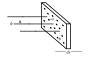
\includegraphics[width=0.8\textwidth]{images/Theory/CrossSectionSchematics.pdf}
    \caption[Cross Section Schematic View]{Shown above is a schematic view of the cross section concept. It depicts a beam of particles $a$ featuring a flux $\phi$ inciding on to a fixed target plate made of material with a width of $dx$. The cross section $\sigma$ is indicated by small areas around every target particle $b$ in the plate.}
    \label{fig:CrossSectionSchematics}
\end{figure}

\subsection{Calculating Cross Sections} \label{sec:CrossSectionCalculation}
In order to calculate cross sections from theoretical models, one first needs to derive Fermi's golden rule, introduced by P. Dirac \cite{GoldenRuleDirac} and named by E. Fermi as it became famous in his lecture on nuclear physics \cite{FermiLecture}. Hereby we will follow a similar strategy as in \cite{ModernParticlePhysics}. We start with the Schr\"odinger equation with a perturbative Hamiltonian $H = H_0 + H_{\text{int}}$, \ie
\begin{equation} \label{eq:PerturbativeSchroedinger}
    i\frac{d}{dt}\ket{\psi(t,\vec{x})} = \left( H_0 + H_{\text{int}} \right) \ket{\psi(t,\vec{x})},
\end{equation}
and then write down $\psi$ as a superposition of the eigenstates of the unperturbed Hamiltonian $\phi_n(t,\vec{x})$ given as
\begin{equation}
    \ket{\psi(t,\vec{x})} = \sum_n c_n(t) e^{-iE_nt} \ket{\phi_n(\vec{x})}.
\end{equation}
With this, we extracted the time dependent part of $\phi_n$ using the exponential term with $E_n$ being the eigenvalue of the $H_0$ operator, \ie $E_n\ket{\phi_n} = H_0\ket{\phi_n}$. If we plug above expression into our Schr\"odinger equation \ref{eq:PerturbativeSchroedinger} we end up with
\begin{equation}
    i\sum_n e^{-iE_nt} \frac{dc_n(t)}{dt} \ket{\phi_n} = \sum_n c_n(t) e^{-iE_nt} H_{\text{int}} \ket{\phi_n}. 
\end{equation}
Now it is beneficial to introduce some boundary conditions for this problem. At $t=0$ we want $\psi$ to be equal to the initial state $\phi_i$, wherefore $c_n(0)=\delta_{ni}$ is a Kronecker delta. We can further assume that the perturbation through $H_{\text{int}}$ is small enough that this still holds true for $t>0$, \ie $c_n(t) \approx \delta_{ni}$. Hence, we write the first order perturbative relation as
\begin{equation}
    i\sum_n e^{-iE_nt} \frac{dc_n(t)}{dt} \ket{\phi_n} = e^{-iE_it} H_{\text{int}} \ket{\phi_i}.
\end{equation}
Since we are interested in an amplitude of a process with an initial state $\ket{\phi_i}$ and a final state $\bra{\phi_f}$ it is appropriate to multiply $\bra{\phi_f}e^{iE_ft}$ to both sides of the equation. As different eigenstates of $H_0$ are perpendicular to one another, \ie $\braket{\phi_a|\phi_b} = \delta_{ab}$, only the $\phi_f$ terms in the sum of the left side remain non-zero. Thus, we end up with
\begin{equation}
    i\frac{dc_f(t)}{dt} = \braket{\phi_f|H_{\text{int}}|\phi_i} e^{-it(E_i-E_f)}
\end{equation}
We already encountered a term of the form like $\braket{\phi_f|H_{\text{int}}|\phi_i}$ in section \ref{sec:InitialAndFinalStates} equation \ref{eq:MatrixElement}; it is akin to a matrix element of an interaction with initial state $\phi_i$ and a final state $\phi_f$. Although in this case here it is not Lorentz invariant, for we derived it via the Schr\"odinger equation, and we name it $\widetilde{T}_{if}=\braket{\phi_f|H_{\text{int}}|\phi_i}$. Next we solve above equation for $c_f$ assuming $H_{\text{int}}$ is constant in the relevant time frame,
\begin{equation}
    c_f(t) = -i\widetilde{T}_{if} \int_{-T}^{T} dt \ e^{-it(E_i-E_f)}.
\end{equation}
Now, $c_f$ constitutes the amplitude of a process where an initial state $\phi_i$ transforms into a final state $\phi_f$. Hence, we can derive the probability of said process to occur by simply squaring the amplitude:
\begin{equation}
    P(i\to f) = \left| c_f(t) \right|^2 = \big| \widetilde{T}_{if} \big|^2 \int_{-T}^{T} dt \int_{-T}^{T} dt^{\prime} \ e^{-it(E_i-E_f)} e^{it^{\prime}(E_i-E_f)},
\end{equation}
where the integral over $dt^{\prime}$ can be solved resulting in a delta distribution term \mbox{$2\pi \delta(E_i-E_f)$}. Furthermore, we are interested in the event rate $\Gamma_{if}$, which is introduced through the relation
\begin{equation}
    d\Gamma_{if} = \frac{P_{if}}{2T} dN_{E_f} =  2\pi \big| \widetilde{T}_{if} \big|^2 \frac{1}{2T} dN_{E_f} \int_{-T}^{T} dt \ e^{-it(E_i-E_f)} \delta(E_i-E_f).
\end{equation}
Here $dN_{E_f}$ is the number of states in phase space available to the final state particle \cite{Perkins, ModernParticlePhysics}. For now we will drop the subscript of $dN$ and continue with
\begin{align}
    \Gamma_{if} &= 2\pi \int \frac{dN}{dE_f}dE_f \ \big| \widetilde{T}_{if} \big|^2 \delta(E_i-E_f) \frac{1}{2T} \int_{-T}^{T} dt \ e^{-it(E_i-E_f)}\nonumber \\
    &= 2\pi \big| \widetilde{T}_{if} \big|^2 \left. \frac{dN}{dE_f} \right|_{E_i} \frac{1}{2T} \int_{-T}^{T} dt \\
    &= 2\pi \big| \widetilde{T}_{if} \big|^2 \left. \frac{dN}{dE_f} \right|_{E_i}. \nonumber
\end{align}
With this we derived Fermi's golden rule, which is also often written with the so-called density of states $dN/dE_f|_{E_i} = \rho(E_i)$. But for our purposes we need to go back to an intermediate step of the golden rule:
\begin{equation} \label{eq:FermiGoldenRule}
    \Gamma_{if} = 2\pi \int dN \ \big| \widetilde{T}_{if} \big|^2 \delta(E_i-E_f).
\end{equation}

As an example, let us consider an interaction between two initial states $a$ and $b$ transitioning into two final states $1$ and $2$, \ie $a + b \to 1 + 2$, as in our previous example for our Feynman diagram in subsection \ref{sec:InitialAndFinalStates}. This means that we need to adjust our transition matrix element with
\begin{equation}
    \widetilde{T}_{if} = \braket{\phi_1\phi_2|\hat{H}_{\text{int}}|\phi_a\phi_b}.
\end{equation}
Furthermore, we also need to extend the delta distribution of equation \ref{eq:FermiGoldenRule} to our four states, \ie $\delta(E_i-E_f) \to \delta(E_a+E_b-E_1-E_2)$. Also, one can show \cite{ModernParticlePhysics} that for our process with an arbitrary number $m$ of final states, $dN$ is given by
\begin{equation} \label{eq:PhaseSpaceParameter}
    dN = \frac{(2\pi)^3}{V}\prod_{f=1}^m\frac{d^3p_f}{(2\pi)^3} \ \delta^{(3)}\left( \vec{p}_a + \vec{p}_b - \sum_{f=1}^m \vec{p}_f \right),
\end{equation}
where $V/(2\pi)^3$ is the volume occupied by a single state, but we set $V=1$ for now. At this point we want our golden rule formula to become Lorentz invariant and we can achieve this by replacing our matrix element $\widetilde{T}_{if}$ by the invariant matrix element we derived in \ref{eq:MatrixElementNeutrino}. For this we need to look at behaviour of the eigenstates $\phi$ after a Lorentz transformation $\phi^{\prime}$. The only difference lies in the normalisation, since
\begin{equation}
    \braket{\phi|\phi} = 1  \quad \longrightarrow \quad \braket{\phi^{\prime}|\phi^{\prime}} = 2E,
\end{equation}
Thus, we have to normalise the same way we did with the ladder operators in equation \ref{eq:aOperators} and get
\begin{equation}
    \phi^{\prime} = \frac{1}{\sqrt{2E}}\phi
\end{equation}
This implies that we are able to relate the invariant matrix element $\mathcal{M}$ with its non-invariant cousin $\widetilde{T}_{if}$ in the following manner:
\begin{equation} \label{eq:MatrixElementRelation}
    \widetilde{T}_{if} = \frac{\mathcal{M}(a+b\to 1+2)}{4\sqrt{E_a E_b E_1 E_2}}.
\end{equation}
Finally, we end up with the event rate of our process by plugging in the phase space parameter of \ref{eq:PhaseSpaceParameter}, and the invariant matrix element from \ref{eq:MatrixElementRelation} into our golden rule \ref{eq:FermiGoldenRule} and get
\begin{equation} \label{eq:EventRateCrossSection}
    \Gamma_{if} = \frac{1}{64\pi^2E_a E_b} \int \frac{d^3p_1}{E_1} \frac{d^3p_2}{E_2} \left|\mathcal{M}(a+b\to 1+2)\right|^2 \delta^{(4)}(p_a+p_b-p_1-p_2)
\end{equation}
Actually, by using the invariant matrix element, the whole equation became Lorentz invariant, since $dp^{\prime}/E^{\prime} = dp/E$.

At this point we are ready to calculate a cross section. As a matter of fact, we already discussed the missing step in the cross section introduction with equation \ref{eq:TotalCrossSectionDef}. We further know how the flux $\phi$ is defined from \ref{eq:Flux}. Thus, it is useful to combine these two equations to
\begin{equation}
    \sigma = \frac{\Gamma}{N_T n_a v_i}
\end{equation}
There is one difference though: in an experiment we need a lot of statistics, thus detectors usually feature high density targets in combination with high luminosity beams. When calculating a cross section theoretically it can be done by considering just one incident and one target particle. Hence, we set $\Gamma\to \Gamma_{if}$, $N_T = 1$, and $n_a = N_a/V = 1/V$. Remember when we set the volume $V = 1$ while calculating the phase space parameter $dN$? It is here, where the volumes cancel out when plugging in $\Gamma_{if}$ derived in equation \ref{eq:EventRateCrossSection}. Therefore, we also set $V = 1$ in this case. As a last step, it is useful to define the incident velocity as the sum of both initial particle's velocity $v_i = v_a + v_b$. With all this we end up with the formula for the cross sections for two initial particles,
\begin{equation}
    \sigma = \frac{\Gamma_{if}}{v_a + v_b}.
\end{equation}
Now we substitute $\Gamma_{if}$ and write the Lorentz invariant cross section as
\begin{equation}
    \sigma = \frac{1}{64\pi^2E_aE_b(v_a+v_b)} \int \frac{d^3p_1}{E_1} \frac{d^3p_2}{E_2} \left|\mathcal{M}\right|^2 \delta^{(4)}(p_a+p_b-p_1-p_2)
\end{equation}
In order to simplify the kinematic part, let us no longer consider an incident and a target particle, but rather look at them in the \gls{cms}. In our example the \gls{cms} implies that the sum of the incoming momenta is zero, whereby, due to momentum conservation, the same is true for the outgoing momenta. In consequence we get $\vec{p}_a = -\vec{p}_b$, and $\vec{p}_1 = - \vec{p}_2$. Let us also introduce the \gls{cms} energy $E_{\text{cms}} \coloneqq E_a + E_b$. Now we can split up the $\delta$-distribution into an energy and a momentum dependent part and integrate
\begin{align}
    \sigma &= \frac{1}{64\pi^2E_aE_b(v_a+v_b)} \int \frac{d^3p_1}{E_1} \frac{d^3p_2}{E_2} \left|\mathcal{M}\right|^2 \delta(E_{\text{cms}}-E_1-E_2) \delta^{(3)}(\vec{p}_1+\vec{p}_2) \nonumber \\
    & = \frac{1}{64\pi^2E_aE_b(v_a+v_b)} \int \frac{d^3p_1}{E_1} \frac{1}{E_2} \left|\mathcal{M}\right|^2 \delta\left( E_{\text{cms}}-\sqrt{m_1^2+\vec{p}_1^{\,2}}-\sqrt{m_2^2+\vec{p}_1^{\,2}}\right) \nonumber \\
    & = \frac{1}{64\pi^2E_aE_b(v_a+v_b)} \int d\Omega \ d|\vec{p}_1| \ \vec{p}_1^{\,2} \left|\mathcal{M}\right|^2 \frac{\delta\left( E_{\text{cms}}-\sqrt{m_1^2+\vec{p}_1^{\,2}}-\sqrt{m_2^2+\vec{p}_1^{\,2}}\right)}{\sqrt{m_1^2+\vec{p}_1^{\,2}}\sqrt{m_2^2+\vec{p}_1^{\,2}}}
\end{align}
For the last integral we parameterised for spherical coordinates, but in order to integrate we need to substitute the integration variable $|\vec{p}_1|$ with
\begin{align}
    u \coloneqq& \ \sqrt{m_1^2+\vec{p}_1^{\,2}} + \sqrt{m_2^2+\vec{p}_1^{\,2}} \nonumber \\
    \Longrightarrow \frac{du}{d|\vec{p}_1|} =& \ \frac{|\vec{p}_1| \left( \sqrt{m_1^2+\vec{p}_1^{\,2}} + \sqrt{m_2^2+\vec{p}_1^{\,2}} \right)}{\sqrt{m_1^2+\vec{p}_1^{\,2}}\sqrt{m_2^2+\vec{p}_1^{\,2}}}
\end{align}
Further, it is useful to introduce $\vec{p}_i \coloneqq \vec{p}_a = -\vec{p}_b$ and $\vec{p}_f \coloneqq \vec{p}_1 = -\vec{p}_2$. In the form factor we find the relation $E_aE_b(v_a+v_b) = E_{\text{cms}}|\vec{p}_i| = \smash{[(\vec{p}_{i\mu} \vec{p}_i^{\,\mu})^2 - m_a^2m_b^2]^{1/2}}$, where the last expression shows the Lorentz invariance of the form factor as it contains invariant four vectors. Thus, our integral takes the form
\begin{align} \label{eq:TotalCrossSectionTheory}
    \sigma &= \frac{1}{64\pi^2E_{\text{cms}}|\vec{p}_i|} \int d\Omega \ du \ \frac{|\vec{p}_f|}{u} \left|\mathcal{M}\right|^2 \delta(E_{\text{cms}}-u) \nonumber \\
    &= \frac{1}{64\pi^2E_{\text{cms}}^2} \frac{|\vec{p}_f|}{|\vec{p}_i|} \int d\Omega \left|\mathcal{M}\right|^2,
\end{align}
and the differential cross section is given by
\begin{equation} \label{eq:DiffCrossSectionTheory}
    \frac{d\sigma}{d\Omega} = \frac{1}{64\pi^2E_{\text{cms}}^2} \frac{|\vec{p}_f|}{|\vec{p}_i|} \left|\mathcal{M}\right|^2.
\end{equation}
There is one more simplification one can apply to the equation above. In the limit where the particle masses can be neglected, the centre of mass frame differential cross section is given by,
\begin{equation} \label{eq:DiffCrossSectionTheoryMassless}
    \frac{d\sigma}{d\Omega} = \frac{1}{64\pi^2E_{\text{cms}}^2} \langle \left|\mathcal{M}\right|^2 \rangle,
\end{equation}
where $\langle \left|\mathcal{M}\right|^2 \rangle$ represents the spin-averaged invariant matrix element squared \cite{ModernParticlePhysics}. More-over, by neglecting particle mass in the \gls{cms} we get $E_a = E_b$. 

So far, all the equations within this section are universally valid for any two-body to two-body interaction (with the exception of the particle mass constraints introduced in the last step). Now it is time to focus again on the main topic of this thesis: the neutrino \gls{cc} cross section. For this reason we go back to the invariant matrix element of the charged current neutrino interaction of equation \ref{eq:MatrixElementNeutrino}. When properly calculating said equation and averaging over the possible spin states of the quarks, we get
\begin{equation}
    \langle \left|\mathcal{M}\right|^2 \rangle = \frac{1}{2} \left( \frac{g_\text{w}^2}{m_W^2} E_{\text{cms}}^2 \right)^2.
\end{equation}
As can be seen, when dealing with small masses, neither the differential cross section nor the spin averaged invariant matrix element exhibit any angle dependency in the centre of mass system. Hence, the integral to calculate the total cross section from equation \ref{eq:DiffCrossSectionTheoryMassless} becomes trivial. By using the Fermi constant as defined in equation \ref{eq:FermiConstant} we get a total cross section of \cite{ModernParticlePhysics}
\begin{equation}
    \sigma(\nu_{\ell}+d \to \ell+u) = \frac{G_\text{F}^2}{\pi} E_\text{cms}^2  \approx \num{1.7e-38} \cdot E_\text{cms}^2 \ \si{\centi\metre\squared}.
\end{equation}
In the second part of above equation, $E_\text{cms}$ has to be given in \si{\giga\electronvolt}. What catches the eye is how small neutrino interaction cross sections are. With typical $E_\text{cms} = \SI{1}{\giga\electronvolt}$, the cross section only amounts to the order of \SI{e-38}{\centi\metre\squared}. This makes neutrino interactions a rare occurrence and their detection challenging. Again, note that this formula only holds true if the particle masses are irrelevant compared to the centre of mass energy, \ie $E_\text{cms} \gg \sum m_i $. Hence, it is best suited to describe electron neutrino, $\nu_e$, interactions. Moreover, due to the assumptions made to derive the invariant matrix element in equation \ref{eq:MatrixElementNeutrino}, it is required that the transferred momentum of the interaction is much smaller than the mass of the $W$-\gls{Boson}, more precisely: $q^2 \ll m_W^2$.

\subsection{Nuclear Effects}
At this point we derived a model for the cross section of a \gls{cc} neutrino interaction with a free down quark. The question now is, how to measure the cross section and verify said model, as there are no free quarks found in nature. The only reasonably stable quark carriers are the two nucleons: the proton $p$ and the neutron $n$, if the latter is bound in an atomic nucleus. Since the cross section is expected to be tiny, we require a high target density in our detector medium in order to achieve an adequate event rate. Hence, high density materials featuring many nucleons are used in modern detectors, \eg argon, the target material of MicroBooNE, features \num{40} nucleons. 

The ultimate goal of every particle physics experiment is to reconstruct all kinematic parameters of the initial particles and the interaction products. In this context, neutrino experiments face a critical difficulty for neutrino beams are not monochromatic, \ie they feature a broad energy spectrum as shown in figure \ref{fig:CrossSectionAndFlux}. Hence, the initial neutrino energy has to be reconstructed from the direct interaction products. Most detectors today are only able to measure the ionisation energy deposited by free or quasi-free charged particles with at best a millimetre spacial resolution (see chapter \ref{sec:LArTPC}). Thus, many of the observed particle traces do not originate directly form the primary interaction vertex but from daughter particles, and even daughters of daughters. For these reasons, neutrino experiments rely heavily on nuclear models for the kinematic reconstruction of the neutrino interaction.
\begin{figure}[htbp]
    \centering
    \includegraphics[width=0.7\textwidth]{images/Theory/CrossSectionGraph.pdf}
    \caption[Beam Fluxes and Neutrino Cross Section Models]{Above figure shows the neutrino flux as a function of neutrino energy for various experiments overlayed by netrino cross section models. The figure is sourced from \cite{ProgressInNuMeasurements}.}
    \label{fig:CrossSectionAndFlux}
\end{figure}

Unfortunately, the \gls{sm} is of little use to model nuclear interactions. The reason for this is the nature of the coupling constant of the strong force, $\alpha_\text{s}$, as it increases with decreasing transferred momentum. For quarks and gluons in a stable bound state like a nucleon, the coupling constant is greater than one, $\alpha_\text{s} > 1$. As established in section \ref{sec:FeynmanGraphs}, the invariant matrix element $\mathcal{M}$ is in fact a power series of Feynman diagrams of different orders and with it also a power series of $\alpha_\text{s}$. Under these circumstances it is not hard to see that that $\mathcal{M} \to \infty$ when $\alpha_\text{s} > 1$. This infinity problem is also called \textbf{running coupling} and can not be solved by renormalisation. In order to still provide a model, theorists resort to so-called \textbf{effective field theories}. These often treat nucleons and \glspl{Meson} as elementary particles, omitting their internal structure. These models are mostly limited to a certain range in transferred momentum and are subject to large systematic uncertainties. In the following paragraphs the most popular models are introduced, relying heavily on the descriptions given by M. Nirkko in his thesis \cite{PhDMartti}.

At neutrino energies in the sub-\si{\giga\electronvolt} range, $q^2$ is too low to break the target nucleus and the neutrino will scatter (quasi-)elastically. In the case of \gls{nc} interactions, neutrinos $\nu_\ell$ can scatter off nucleons $N$ elastically (neutral current elastic scattering, see figure \ref{fig:NCEL}):
\begin{equation}
    \nu_\ell + N \to \nu_\ell + N.
\end{equation}
Here, $\ell$ stands for any of the three lepton flavours. In the low energy range ($E_\nu \lesssim \SI{1}{\giga\electronvolt}$) where the neutrino energy is large enough to produce a charged lepton, but $q^2$ exchanged by the weak \gls{Boson} is not sufficient to break the target nucleus, \gls{ccqe} scattering \cite{NuQuasiElasticScattering} on neutrons (figure \ref{fig:CCQE}) is the dominant process:
\begin{equation}
    \nu_\ell + n \to \ell^- + p.
\end{equation}
These interactions are important to neutrino physics for a number of reasons. Most notably, their nature as two-body interactions enable the kinematics to be fully reconstructed: Assuming an initial nucleon at rest, the neutrino energy can be inferred:
\begin{equation}
    E_\nu = \frac{m_n E_\ell + \frac{1}{2}(m_p^2 + m_n^2 + m_\ell^2)}{m_n - E_\ell + p_\ell \cos{(\theta_\ell)}},
\end{equation}
where $m_x$ is the mass of the nucleons ($n$ or $p$) or the produced lepton $\ell$. Moreover, $p_\ell$ and $E_\ell$ are the lepton momentum and energy, respectively. Finally, $\theta_\ell$ denotes the scattering angle with respect to the incident neutrino momentum. However, above formula becomes significantly more complicated when the nucleon is not free but bound in a large atomic nucleus like argon \cite{PhDMartti}. This theory was extended to larger nuclei with the \gls{rfg} model, which treats nucleons as quasi-free with Fermi momentum, in the mean field of the nucleus, where the nuclear parameters are tuned to electron scattering data \cite{ProgressInNuMeasurements}. However, the predictions of said model are quite poor leading to MiniBooNE's ``\gls{ccqe} puzzle'' \cite{AxialMassMiniBooNE}, when a significantly greater cross section was extracted from the data than seen in earlier experiments using deuterium, \ce{^2H}, as their target material. Evidently, the non-trivial nuclear effects at the \gls{ccqe} energy scale must not be omitted.
\begin{figure}[htbp]
    \centering
    \subfloat[Neutral Current Elastic Scattering][Neutral current elastic scattering]
    {
        \includegraphics[width=0.49\textwidth]{images/Theory/NCEL.pdf}
        \label{fig:NCEL}
    }
    \subfloat[Charged Current Quasi-Elastic Scattering][Charged current quasi-elastic scattering]
    {
        \includegraphics[width=0.49\textwidth]{images/Theory/CCQE.pdf}
        \label{fig:CCQE}
    }
    \caption[MicroBooNE TPC]{Shown above are the Feynman diagrams of the neutral current elastic scattering in \subref{fig:NCEL}, and of the charged current quasi-elastic scattering \subref{fig:CCQE}. As an example, the primary particle is chosen to be $\nu_\mu$. Sourced from \cite{PhDMartti}.}
    \label{fig:NCELandCCQE}
\end{figure}

At intermediate neutrino energies (\SIrange{1}{10}{\giga\electronvolt}), higher values of $q^2$ become available, and neutrinos can begin to scatter inelastically. While the leptonic side of the interaction does not change, on the hadronic side the nucleon can be boosted into an excited state (baryonic resonance, \eg \ch{N^*}, $\Delta$). These resonances then decay back to a nucleon in the ground state, often accompanied by a pion. However, depending on the type of resonance a variety of final states is possible, including multiple pions, kaons or a radiative photons. These interactions are known as \gls{res}, the most common result being the production of a single pion ($\num{1}\pi$). A typical resonant interaction is
\begin{equation}
    \nu_\ell + p \to \ell + \Delta^{++} \to \ell + \pi^+ + p^\prime,
\end{equation}
whith the $W$-\gls{Boson} converting the down-quark in the initial proton to an up-quark, resulting in a seemingly symmetric state ($\Delta^{++} = uuu$) which decays into a proton and a pion (figure \ref{fig:CCRES}) \cite{PhDMartti}.
\begin{figure}[htbp]
    \centering
    \includegraphics[width=0.5\textwidth]{images/Theory/CCRES.pdf}
    \caption[Charged Current Resonant Interaction]{Depicted here is the Feynman diagram for a charged current resonant interaction: A muon-neutrino interacts with a proton, causing it to reach an excited state ($\Delta^{++}$ resonance), which decays into a proton and a single pion \cite{PhDMartti}.}
    \label{fig:CCRES}
\end{figure}

At high neutrino energies ($E_\nu \gtrsim \SI{10}{\giga\electronvolt}$), values of $q^2$ can become high enough for the internal structure of the nucleon to be resolved. The neutrinos can then scatter directly off the quarks within, which is known as \gls{dis}. The process is not limited to valence quarks; scattering can also occur off ``sea quarks'' that continuously pop in and out of existence in a nucleon. A consequence of this interaction is inevitably the break up of the target nucleon: As the struck quark recoils, the nucleon fragments and the strong forces between quarks result in hadronisation, \ie the production of multiple hadrons. The final state often includes multiple pions and nucleons exiting the shattered nucleus (see figure \ref{fig:DIS}), resulting in events with high track multiplicity \cite{PhDMartti}.
\begin{figure}[htbp]
    \centering
    \includegraphics[width=0.5\textwidth]{images/Theory/DIS.pdf}
    \caption[Charged Current Deep Inelastic Scattering]{Above is a Feynman diagram for a neutrino interacting via charged current deep inelastic scattering. The nucleon $N$ is shattered, causing multiple pions $n\pi^{\pm,0}$ and other hadrons $X$ to be produced \cite{PhDMartti}.}
    \label{fig:DIS}
\end{figure}

The cross section of the three described (anti-)neutrino interaction modes as a function of neutrino energy is depicted in figure \ref{fig:CrossSectionDistribution}. It shows experimentally determined data points as well as the above-described model predictions (solid lines). As can be seen, the models do not match the data points in many cases. This state of affairs, especially the \gls{ccqe} discrepancies, prompted many particle physicists to rethink these interaction categories as a whole. This new approach will be described in the next paragraph.
\begin{figure}[htbp]
    \centering
    \subfloat[Neutrino Cross Section][Neutrino cross section]
    {
        \includegraphics[width=0.45\textwidth]{images/Theory/NuCrossSection.pdf}
        \label{fig:NuCrossSection}
    }
    \subfloat[Antineutrino Cross Section][Antineutrino cross section]
    {
        \includegraphics[width=0.45\textwidth]{images/Theory/AntiNuCrossSection.pdf}
        \label{fig:AntiNuCrossSection}
    }
    \caption[Neutrino and Antineutrino Cross Section]{Shown here are experimentally observed cross sections for \subref{fig:NuCrossSection} neutrino and \subref{fig:AntiNuCrossSection} antineutrino interactions. The models of the dominant reaction types and the total cross section are shown as solide lines as a function of energy. Sourced from \cite{PhDMartti} and influenced by \cite{CrossSectionReview}.}
    \label{fig:CrossSectionDistribution}
\end{figure}

As established before, hadrons produced within neutrino interactions can rescatter before exiting the nucleus, thereby significantly modifying the outgoing hadron composition and kinematics that are experimentally observed. Such rescattering processes are typically known as \gls{fsi}. Since it is impossible to look inside the nucleus to see what is going on (as shown schematically in figure \ref{fig:FSI}), these interactions can only be inferred by nuclear models, and by precisely measuring the final state kinematics of any observable particles leaving the nucleus \cite{PhDMartti}. This means that we are unable to reasonably measure \gls{ccqe}, instead we can observe an event topology with a single charged lepton and no pions (\gls{cc}$0\pi$). This certainly contains \gls{qe} events but neither exclusively nor completely. As we do not want to assume a model for these processes, we can only measure cross sections for a given post-\gls{fsi} signature. Mathematically these measured cross sections are defined as \cite{ProgressInNuMeasurements} 
\begin{equation}
    \tilde{\sigma}_n(\mathbf{k}) = \sum_{m} \int_{E_\text{min}}^{E_\text{max}} dE_\nu \ \sigma_m(E_\nu,\mathbf{k}^{\prime}) \text{FSI}(\mathbf{k}^{\prime},\mathbf{k}),
\end{equation}
where $E_\nu$ denotes the neutrino energy in the $E_\text{min}$ to $E_\text{max}$ range output by the neutrino beam line. $\sigma_i$ is the cross section of the true process categories, and the function $\text{FSI}(\mathbf{k^\prime},\mathbf{k})$ transforms the kinematics of the initial interaction products $\mathbf{k}^\prime$ into the kinematics of the post-\gls{fsi} particles $\mathbf{k}$. These kinematics $\mathbf{k}^{(\prime)}$ are mostly given by the momentum and the scattering angle of a particle, \eg $p_\mu^{(\prime)}$ and $\theta_\mu^{(\prime)}$. Note, not only did we change the definition of the cross section but we also changed the definition of the final state: it is now the particles as measured in the detector and not as created by the primary neutrino interaction. This change in philosophy also meant to collaborate with nuclear physicists to create the needed models \cite{NuclearModels,GIBUU}. At this point we can also better understand the main topic of this thesis, \ie the $\nu_\mu$ \gls{cc} inclusive cross section measurement. This event topology describes a \gls{cc} final state, with any hadronic final state configuration (including no hadrons), meaning that every neutrino event with a muon is counted. In view of the new nuclear models, the \gls{cc} inclusive cross section is given by the sum of all possible \gls{cc} related sub-processes, thus it can be used to tune the initial interaction model. The \glspl{fsi} do not matter in this case as we accept all of them with the inclusive event signature \cite{NuclearModels,GIBUU}.
\begin{figure}[htbp]
    \centering
    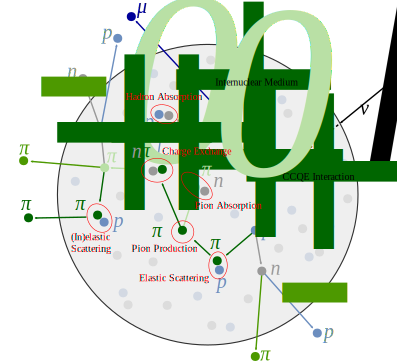
\includegraphics[width=1.0\textwidth]{images/Theory/FSI.pdf}
    \caption[Final State Interaction Example]{Illustrated here, is an example of \glspl{fsi}. First, the inciding muon neutrino $\nu_\mu$ represented by the black arrow followed by the dashed black line scatters via a \gls{ccqe} interaction with a neutron of an argon nucleus. The produced negatively charged muon (indigo) and the positively charged proton (light blue) traverse through the nuclear medium and are subject to nuclear effects (nuclear binding energy, Coulomb distortion, etc.). In the second step, the proton can undergo various types of \glspl{fsi} which may lead to even more \glspl{fsi} such as (in)elastic scattering, pion production, hadron absorption and charge exchange. The pions ($\pi^+$, $\pi^-$, and $\pi^0$) in this figure are shown in dark, lighter, and light green, respectively \cite{CrossSectionFSI}.}
    \label{fig:FSI}
\end{figure}

\subsection{Measuring Cross Sections} \label{sec:MeasuringCrossSection}
Every cross section measurement starts with a measured event rate in a detector. Said rate is dependent on the detector itself, the event reconstruction, and the event selection process. In other words, the rate may vary strongly for every analysis. To receive universally comparable results, we use \gls{mc} models to quantify the effects of this selection bias. In order to achieve this, whole events have to be simulated starting with the neutrino interaction and ending with the readout electronics response of the detector. These \gls{mc} events should now be almost indistinguishable from raw events measured with the detector. Hence, these models need to be of excellent quality. The events are then subjected to the very same reconstruction and selection algorithms as the real detector data. The \gls{mc} data sets provide vital truth information which can then be compared to the selected reconstruction events. Two often used quantities to determine the quality of a selection process are the purity $p$ and the efficiency $\epsilon$. The purity is a measure of how many of the selected events are true signal events, and the efficiency indicates how many of the true signal events were selected, \ie 
\begin{equation}
    p \coloneqq \frac{\text{\# selected signals}}{\text{\# total selected}}, \qquad \epsilon \coloneqq \frac{\text{\# selected signals}}{\text{\# total signals}}.
\end{equation}
Both variables are often used to optimise the cut values of the various selection steps. The most prominent method is to maximise the products of the two \cite{EfficiencyTimesPurity}, \ie $\max{(p\epsilon)}$, as will be shown in chapter \ref{sec:FistCCInclusive}. After selection process, the truth information allows us to distinguish between the number of selected signal events, $S$, and the number of selected background events $B$. In total both amount to the total number of selected events $N = S+B$.

The results of a cross section analysis are usually distributions in at least one kinematic parameter $k$. Said distributions are in histogram form, \ie they are binned. Consequently, the selection numbers also need to be binned and we get $N_i = S_i + B_i$. When dealing with a \gls{mc} sample, it is useful to compare the reconstructed with the true distributions. This is done with the so-called \textbf{smearing matrix} $U_{ij}$, which describes the mapping between a true bin $j$, and a reconstructed bin $i$. It is defined as
\begin{equation} \label{eq:SmearingMatrix}
    U_{ij} \coloneqq \frac{\text{\# selected reconstruction events in bin }i \text{ with a truth value in bin }j}{\text{\# generated truth events in bin }j}.
\end{equation} 
From this, the bin efficiency $\epsilon_j$ can be extracted with $\epsilon_j = \sum_i U_{ij}$. This indicates that the selection efficiency is also incorporated into the smearing matrix.

With these tools we are now able to derive the formula to calculate differential cross sections from event rates. As a matter of fact, we were already very close with the differential cross section formula of equation \ref{eq:DiffCrossSection}, although in practice one uses binned histograms, instead of a continuous function. This means that $d\sigma/dk$ is transformed to $\delta\sigma/\delta k_j$, where $\delta k_j$ is equivalent to the width of bin $j$. As is indicated by the bin index $j$, we will transform the differential cross section from reconstructed space into true space to allow for comparisons with cross section models. Therefore, the smearing matrix needs to be inverted ($U_{ij}^{-1}$), but this often leads to large fluctuations in the resulting matrix elements, as statistical uncertainty in the reconstruction space is blown up by the inversion \cite{ProgressInNuMeasurements}. Sometimes $U_{ij}$ is not even invertible, hence, the pseudoinverse $\widetilde{U}^{-1}_{ij}$, also called \textbf{unfolding matrix}, is utilised to map the reconstruction bis into true bins. Now, the formula to extract the differential cross section from detector data is given by
\begin{equation} \label{eq:CrossSectionMeasurement}
    \frac{\delta\sigma^\text{real}}{\delta k_i} = \frac{\sum_j \widetilde{U}^{-1}_{ij} \left( N_i^\text{real} - B_i \right)}{\delta k_i \Phi_{\nu} N_T}.
\end{equation}
Note, that the neutrino beam flux $\Phi_{\nu}$ as well as the number of target nucleons are constants and remain unbinned as in equation \ref{eq:DiffCrossSection}. Furthermore, it is important to stress that $N_i^\text{real}$ is the number of selected real world event in bin $i$. Depending on the detector technology, the background $B_i$ can be a combination of expected background determined from the \gls{mc} model and real world background measurements.

Now let us take a step back and have a look at the bigger picture of measuring a cross section. The goal of a cross section measurement ought to be the comparison of real world data with \gls{mc} models in order to validate or refute them. For this purpose, our data needs to model independent, otherwise we might introduce a bias. However, the unfolded cross section method discussed above does not fulfil the model independence requirements. In this case, model dependency is introduced with the smearing matrix $U_ij$ and background predictions in $B_i$, when a \gls{mc} neutrino generator is used at the beginning of the simulation process. This generator often even uses the models we use to compare the data to. How large this bias really is, has yet to be investigated \cite{ForwardFolding}. Nevertheless, it might be a good idea, to remove as much model dependence as possible from a cross section analysis. This exact philosophy led to the development of forward-folding analysis methods. The idea here is to use the raw real world data selection $N_i^\text{real}$ as is and forward-fold the \gls{mc} selection to resemble the data. In mathematical form forward-folding is described by \cite{CRTThomasPhD}
\begin{equation} \label{eq:ForwardFolding}
    N_i^\text{mc} = \Phi_\nu N_T \sum_j U_{ij} \sigma_j^\text{mc} + B_i
\end{equation}
In this case, $N_i^\text{mc}$ is the number of events in reconstructed space as predicted by the \gls{mc} simulation which will be compared to $N_i^\text{real}$. Moreover, $\sigma_j^\text{mc}$ is the \gls{mc} cross section model in true space which we want to compare our data to. With this approach, we keep the model dependencies on the \gls{mc} side of the comparison. As can be seen, forward-folding also spares us from inverting $U_{ij}$ which is proven to be statistically advantageous \cite{ForwardFolding}. However, there are also disadvantages, mostly of political nature. The first problem is already represented by the formula above. It indicates a shifts of responsibility for achieving model comparability from the experimentalist to the modellers. So far, the modellers' tools produce real cross section distributions which now need to be forward-folded. This only gets more complicated once systematic uncertainties enter the game. With this arises the next problem: people are simply not used to forward-folding, these distributions do not make sense to them. Still, in this thesis all cross section related measurements make use of the forward folding method. The results of said measurements are found in the chapters \ref{sec:FistCCInclusive} and \ref{sec:NewCCInclusive}.

\end{fmffile}


% TODO Find Place for this discription
% \section{Neutrino Properties}
% There are three experimentally confirmed neutrino flavours in the \gls{sm}: the electron neutrino $\nu_e$, the muon neutrino $\nu_\mu$, and the tau neutrino $\nu_\tau$. According to the \gls{sm} all neutrino flavours have a corresponding antiparticle which are represented by the symbols $\bar{\nu_e}$, $\bar{\nu_\mu}$, and $\bar{\nu_\tau}$. Neutrinos are spin-\textonehalf{} particles (\glspl{Fermion}) and belong to the group of leptons in the \gls{sm}. They hold neither electrical, nor color charge.  Neutrinos exhibit unique behaviour as particles. For instance, they only interact through weak interaction by exchanging on of the three gauge \glspl{Boson} $W^{\pm}$ and $Z_0$. They are also assumed to have the lowest masses of any \glspl{Fermion} in the \gls{sm}, with the most recent upper limit of $m_{\nu_e} < \SI{0.8}{\electronvolt}$ (\SI{90}{\percent} \gls{cl}) \cite{NeutrinoMass}. This leads to neutrino oscillation, which by itself is a very particular occurrence only observed in neutrinos and will be discussed later in this section. Furthermore, neutrinos seem to have a unique chirality property, \ie there are only neutrinos with left-handed chirality (see section \ref{sec:WeakInteractionTheory}).
% % TODO Mention very low cross section
% 
% % TODO Find a place for this discription
% % TODO reference to momentum and angular momentum conservation of the lagrangian
% \subsection{Parity, Charge Conjugation, and Time Reversal}
% The very backbone of particle physics is the concept of symmetry or invariance of equations under various operations such as rotations or translations in spacetime. In general, symmetries are closely linked to conservation laws. In case of rotations and translations the linked conserved properties are angular- and linear momentum respectively, as mentioned in section \ref{sec:StandardModel}. Three important discrete symmetries are parity, charge conjugation, and time reversal. They are introduced through transformation operators and often used in combination with each other. The parity transformation inverts the spacial coordinates, charge conjugation transforms a particle into its antiparticle, and time reversal inverts the time line.
% 
% As mentioned above the parity transformation causes an inversion of all spatial coordinates $(x,y,z) \to (-x,-y,-z)$. Thus we introduce an operator $\mathcal{P}$ with the following properties:
% \begin{equation}
%     \mathcal{P}\psi(t,x,y,z) = \psi(t,-x,-y,-z).
% \end{equation}
% $\mathcal{P}$ is an unitary operator and produces the eigenvalues $P = \pm1$. This can be shown with two simple example, for simplicity only in one dimension:
% \begin{align}
%     \psi(x) &= \cos(x), \nonumber \\
%     \mathcal{P}\psi(x) &= \psi(-x) = \cos(-x) = \cos(x) = \psi(x), \nonumber \\
%     \Rightarrow P &= +1. \nonumber
% \end{align}
% Thus follows, the cosine function has a parity of $+1$, also called even parity. If we do the same with the sine function we get
% \begin{align}
%     \psi(x) &= \sin(x), \nonumber \\ 
%     \mathcal{P}\psi(x) &= \psi(-x) = \sin(-x) = -\sin(x) = -\psi(x),  \nonumber \\
%     \Rightarrow P &= -1. \nonumber
% \end{align}
% So, the sine function has a parity of $-1$ or odd parity. Sometimes, if $P \neq \pm1$, parity has no defined eigenvalue, \eg
% \begin{align}
%     \psi(x) &= \cos(x) + \sin(x), \nonumber \\
%     \mathcal{P}\psi(x) &= \cos(x) - \sin(x) \neq \pm \psi. \nonumber
% \end{align}
% In this case $\mathcal{P}$ only inverts the coordinates but does create an eigenvalue $P$ infront of the wave function \cite{Perkins}. 
% 
% How is this parity operator tied to a symmetry in particle physics? To answer this question we need to consider particle interactions: if they could occur regardless of the space coordinate inversion, parity is conserved. To the best of our experimental knowledge parity is conserved in all strong and \gls{em} interactions \cite{StandardModel}. It was long believed that parity invariance poses an universal law valid for all particle interactions. In 1956, however, T.D. Lee and C.N. Yang \cite{ParityLeeYang} suspected that parity is not conserved in weak interactions, which was later confirmed by C.S. Wu \cite{ParityWu} in her famous experiment. This originates from the chirality and helicity of the neutrino and the existence of only one handedness which will be discussed in the next section (\ref{sec:ChiralityHelicity}). As R. Mann put it in his Book \cite[Nature is not mirror-symmetric - parity is violated!]{StandardModel}.
% 
% Charge conjugation transforms any state into a state with reversed charge, while energy, momentum, spin, and mass stay the same. In other words each particle $\ket{p}$ gets transformed into its anti-particle $\ket{\bar{p}}$ and vice versa. Therefore the charge conjugation operator $\mathcal{C}$ is introduced,
% \begin{equation}
%     \mathcal{C} \ket{p} = \ket{\bar{p}} \quad \text{\eg} \quad \mathcal{C} \ket{\pi^+} = \ket{\pi^-}.
% \end{equation}
% $\mathcal{C}$ is, as $\mathcal{P}$, a unitary operator and exhibits also the eigenvalues $C = \pm 1$. However, unlike parity, most particles are not eigenstates of $\mathcal{C}$ because a particle is not the same eigenstate as its antiparticle ($\ket{\nu} \neq \pm\ket{\bar{\nu}}$). Hence, $\mathcal{C}$ only produces eigenvalues on particle eigenstates that are their own antiparticle, because eigenvalue equation for $\mathcal{C}$ requires
% \begin{equation}
%     \mathcal{C} \ket{p} = \ket{\bar{p}} = \pm \ket{p}.
% \end{equation}
% Only a hand full of particles, all of the \glspl{Boson}, meet said requirement: $\gamma$, $\pi^0$, $\eta$, $\eta^{\prime}$, $\rho$, $\phi$, and $J/\psi$ \cite{StandardModel}.
% 
% The charge conjugation symmetry by itself is adhered to in \gls{em} and strong interactions. However, it is not a symmetry of all weak interactions since $\mathcal{C}$ applied to a left-handed neutrino, would result in a left-handed anti-neutrino \ie a neutrino with opposite weak charge. Therein lies the same problem as with parity, left-handed anti-neutrinos are not observed in nature \cite{StandardModel}. What would happen if we combined the two symmetries, \eg
% \begin{equation} \label{eq:NuCPViolation}
%     \mathcal{CP} \ket{\nu} = \ket{\bar{\nu}}.
% \end{equation}
% Here, $\mathcal{P}$ transforms a left-handed neutrino into a right-handed one. Thereafter $\mathcal{C}$ transforms the right-handed neutrino into a right-handed antineutrino. This seems to work, but there is a catch: a general CP-symmetry in all particle physics processes would imply a perfect balance of matter and antimatter in the universe which in itself is a contradiction to humanity's very existence. In this sense unsurprisingly, CP-violation was first found in the decay of neutral kaons $K^0$ and $\bar{K}^0$, notably again a week interaction \cite{CP-Violation}. The measured asymmetry, is so small (of the order of \num{1e-3}) that one could state: $\mathcal{CP}$ is almost conserved. So far CP-violation is only mesured in baryon decays. In the lepton sector CP-violation is expected to be the tied via a see-saw mechanism with the baryon sector \cite{NeutrinoCPViolation}. Therefore above equation \ref{eq:NuCPViolation} is invalid by a small fraction. Neutrino models include CP-violation (see neutrino mixing in section \ref{sec:MixingOscillation}), although measuring it is deemed very challenging. 
% % TODO Check the order of cp violation 10^-3 or even smaller
% 
% Time reversal transformation causes an inversion of the time component of a wave function, \ie $t \to -t$, and is introduced through time reversal operator $\mathcal{T}$:
% \begin{equation}
%     \mathcal{T}\psi(t,x,y,z) = \psi(-t,x,y,z).
% \end{equation}
% With time, the operator also inverts all momenta as well as spin. It is probably the most abstract of the three introduced symmetries, as the ever expanding universe or the second law of thermodynamics and its associated concept of ever increasing entropy affirm the existence of irreversible processes in physics. They are clear indicators of the unidirectionality of time and thus a universal time reversal symmetry can not exist on a macroscopic level; for example while reversing time the universe would not expand anymore as it does now, but rather contract. At the microscopic level, which particle physics is definitely a part of, the situation is quite different and there are time reversible processes like the scattering of a neutron $n$ and a proton $p$ to produce deuteron $D$  and a photon $\gamma$:
% \begin{equation}
%     n + p \rightarrow D + \gamma \Leftarrow \mathcal{T} \Rightarrow D + \gamma  \rightarrow n + p. \nonumber
% \end{equation}
% In this case the rate of both processes is the same for corresponding conditions of energy and momenta and they are therefore T-invariant. Moreover, all experiments seem to confirm time reversal symmetry for strong and \gls{em} interactions. Unfortunately it is hard to measure T-invariance in weak interactions and thus far experiments have not produced any results, so we can not discuss the implication of time reversal for neutrinos (which makes me a sad panda).
% 
% Nevertheless, we can again take a look at a combination of symmetries. So let us consider the combination of all three, \ie the CPT-Symmetry first introduced by J. Schwinger \cite{CPT-Invariance}. It is deemed to be one of the fundamental laws of particle physics that CPT-invariance holds for all particle interactions. This law is called the CPT theorem and can be derived using assumptions of Lorentz invariance, quantum field theory. Therefore, if CPT-violation were detected quantum field theory would crumble down as a valid description of nature and would hint at beyond standard model physics. CPT-invariance has several implications:
% \begin{enumerate}
%     \item A Particle and its antiparticle must have the same mass
%     \item A Particle and its antiparticle must have the same lifetimes
%     \item A Particle and its antiparticle must have the same magnetic moments
% \end{enumerate}
% So far, measuring these quantities for several particles and their antiparticles resulted in confirmation of CPT-invariance. Since CPT theorem seems to hold true and CP-violation is detected in weak interactions , logic dictates, that weak interaction must violate the T-symmetry too \cite{Perkins,Griffiths,StandardModel}.
% 
% % TODO Find a place for this discription
% \subsection{Chirality and Helicity} \label{sec:ChiralityHelicity}
% After the discovery of parity violation in weak interactions two concepts became ubiquitous in particle physics: helicity and chirality, both describing the spin rotation properties of particles. The helicity operator is simply defined as the projection of spin $\vec{S}$ of a particle onto its three momentum $\vec{p}$:
% \begin{equation}
%     \mathpzc{h} \coloneqq 2\frac{\vec{S}\cdot\vec{p}}{\left| \vec{p} \right|},
% \end{equation}
% where the factor 2 is used to follow normalisation conventions for spin-\textonehalf{} particles. The operator $\mathpzc{h}$ produces the eigenvalues of $h = +1$ for right-handed, and $h = -1$ for left-handed particles. Figure \ref{fig:NeutrinoHelicity} visualises above equation in a less abstract manner. Chirality, on the other hand, is an intrinsic property of a particle depending on the four-momentum $p$ incorporated in the Dirac spinors $u(p)$ and $v(p)$. These chiral Dirac spinors are discussed in sections \ref{sec:DiracSpinors} as well as \ref{sec:WeakInteractionTheory} and are listed in table \ref{tab:ChiralSpinors}. While the handedness definition of helicity is the same for particles and antiparticles, the sign flips in case of chirality.
% \begin{figure}[htbp]
%     \centering
%     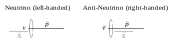
\includegraphics[width=1.0\textwidth]{images/Theory/NeutrinoHelicity.pdf}
%     \caption[Helicity of Neutrinos and Anit-Neutrinos]{The helicity states of neutrinos and anti-neutrinos are depicted here, while $\vec{p}$ indicates the momentum and $\vec{S}$ the spin of the particle. For neutrinos the spin is always anti-parallel to the momentum, while for anti-neutrinos they are both parallel. Looking at above picture it becomes obvious why a space coordinate inversion would fail and thus why parity is violated.}
%     \label{fig:NeutrinoHelicity}
% \end{figure}
% For massless particles chirality and helicity are equal and opposite for massless antiparticles. So if a massless left-handed neutrino created, it will exhibit the same helicity for all observers regardless of their inertial reference frame. But for massive particles helicity is not a Lorentz-invariant quantity. Thus an observer could overtake a massive neutrino in flight, which would change the direction of $\vec{p}$ by \SI{180}{\degree} leaving the spin unchanged. Said observer would therefore see the prohibited state of a right-handed neutrino. Hence neutrinos were long belived to be massles yet in 1998 the Super-Kamiokande observed neutrino oscillation \cite{NuOscillationDiscovery} and thus demonstrated that ther is a mass difference between neutrinos (will be properly discussed section \ref{sec:MixingOscillation}). Today it is established that there are three neutrinos all differing in mass wherefore at least two of those masses must be non-zero. For this reason one could imagine an experiment where the target particle would catch up with a neutrino from behind. With this direct persuit method one could measure the helicity reversal and the absolute mass of a neutrino as well, though it would be extremly hard to produce such an experiment. First it would requires very high energy electron beams in the order of \SI{10}{\tera\electronvolt} and second both, neutrino and electron beams would require extremely high luminosity, due to the low cross section of neutrino interactions \cite{NeutrinoHelicityChirality}. Nevertheless there is a feasable to perform the measurement through neutrinoless double beta decay, which we will explore in the next section. 
% 
% \subsection{Dirac - or Majorana Fermion} \label{sec:DiracOrMajorana}
% There is a way out of the contradiction that there are only left-handed neutrinos (right-handed antineutrinos) and that neutrinos have non-zero mass. In 1937 Ettore Majorana hypotesised a fermion that is its own anitparticle \cite{MajoranaFermionTheory}. So far there are only a fiew \glspl{Boson} with this property and we alredy explored them while discussing charge conjugation above.
% 
% \begin{figure}[htbp]
%     \centering
%     \subfloat[Double-Beta Decay][Double-Beta Decay]
%     {
%     \begin{fmffile}{feynman/DoubleBeta}
%     \fmfset{arrow_len}{2.5mm} % smaller arrows, default 4mm
%     \fmfset{zigzag_width}{1thick}
%     \fmfset{dash_len}{1.5mm}
%         \fmfframe(30,30)(30,30){
%         \begin{fmfgraph*}(120,120)
%             \fmfstraight
%             \fmfleft{i1,i2,i3,i4}
%             \fmfright{o1,o2,o3,o4,o5,o6}
%             % lower fermions
%             \fmfv{label=$\bar{\nu}_e$,label.angle=-20,label.dist=1mm}{o2}
%             \fmfv{label=$e^-$,label.angle=20,label.dist=1mm}{o3}
%             \fmf{fermion,tension=1}{o2,v2,o3}
%             % upper fermions
%             \fmfv{label=$\bar{\nu}_e$,label.angle=-20,label.dist=1mm}{o4}
%             \fmfv{label=$e^-$,label.angle=20,label.dist=1mm}{o5}
%             \fmf{fermion,tension=1}{o4,v3,o5}
%             % Phantoms
%             \fmf{phantom}{i1,v2,v3,i4}
%             \fmf{phantom,tension=2}{i1,v1} % to help \quark
%             \fmf{phantom,tension=2}{i4,v4} % to help \quark
%             \fmf{phantom}{v1,o1} % to help \quark
%             \fmf{phantom}{v4,o6} % to help \quark
%             % virtices
%             \fmfv{decor.shape=circle,decor.filled=full,decor.size=1thick}{v2}
%             \fmfv{decor.shape=circle,decor.filled=full,decor.size=1thick}{v3}
%             \fmffreeze
%             % bosons
%             \fmf{zigzag,label=$W^{-}$,label.side=left,label.dist=1mm}{v1,v2} % lower
%             \fmf{zigzag,label=$W^{-}$,label.side=right,label.dist=1mm}{v4,v3} % upper
%             % lower quarks
%             \fmfv{l=$n$\mylbrace{30}{-7}{2},l.d=16,l.a=-160}{i1}
%             \fmfv{l=\myrbrace{30}{-7}{2}$p$,l.d=16,l.a=-20}{o1}
%             \quark{qldi}{$d$}{0,1}{1.00,1}{0,  0}{left} {0, 0}{0,0}{i1,v1}
%             \quark{qlei}{$d$}{0,1}{1.00,1}{0, -9}{left} {0, 0}{0,0}{i1,v1}
%             \quark{qlfi}{$u$}{0,1}{1.00,1}{0,-18}{left} {0, 0}{0,0}{i1,v1}
%             \quark{qldo}{$u$}{0,1}{1.00,1}{0,  0}{right}{0, 0}{0,0}{v1,o1}
%             \quark{qleo}{$d$}{0,1}{1.00,1}{0, -9}{right}{0, 0}{0,0}{v1,o1}
%             \quark{qlfo}{$u$}{0,1}{1.00,1}{0,-18}{right}{0, 0}{0,0}{v1,o1}
%             % upper quarks
%             \fmfv{l=$n$\mylbrace{30}{28}{2},l.d=16,l.a=-160}{i4}
%             \fmfv{l=\myrbrace{30}{28}{2}$p$,l.d=16,l.a=-20}{o6}
%             \quark{qudi}{$d$}{0,1}{1.00,1}{0,  0}{left} {0, 0}{0,0}{i4,v4}
%             \quark{quei}{$d$}{0,1}{1.00,1}{0, +9}{left} {0, 0}{0,0}{i4,v4}
%             \quark{qufi}{$u$}{0,1}{1.00,1}{0,+18}{left} {0, 0}{0,0}{i4,v4}
%             \quark{qudo}{$u$}{0,1}{1.00,1}{0,  0}{right}{0, 0}{0,0}{v4,o6}
%             \quark{queo}{$d$}{0,1}{1.00,1}{0, +9}{right}{0, 0}{0,0}{v4,o6}
%             \quark{qufo}{$u$}{0,1}{1.00,1}{0,+18}{right}{0, 0}{0,0}{v4,o6}
%         \end{fmfgraph*}
%         }
%         \end{fmffile}
%         \label{fig:FeynmanDoubleBetaDecay}
%     }
%     \subfloat[Neutrinoless Double-Beta Decay][Neutrinoless Double-Beta Decay]
%     {
%     \begin{fmffile}{feynman/NulessDoubleBeta}
%     \fmfset{arrow_len}{2.5mm} % smaller arrows, default 4mm
%     \fmfset{zigzag_width}{1thick}
%     \fmfset{dash_len}{1.5mm}
%         \fmfframe(30,30)(30,30){
%         \begin{fmfgraph*}(120,120)
%             \fmfstraight
%             \fmfleft{i1,i2,i3,i4}
%             \fmfright{o1,o2,o3,o4}
%             % lower fermions
%             \fmfv{label=$e^-$,label.angle=0,label.dist=1mm}{o2}
%             \fmf{fermion,tension=2}{v2,o2}
%             % upper fermions
%             \fmfv{label=$e^-$,label.angle=0,label.dist=1mm}{o3}
%             \fmf{fermion,tension=2}{v3,o3}
%             % phantoms
%             \fmf{phantom}{i1,v2,v3,i4}
%             \fmf{phantom,tension=2}{i1,v1} % to help \quark
%             \fmf{phantom,tension=2}{i4,v4} % to help \quark
%             \fmf{phantom}{v1,o1} % to help \quark
%             \fmf{phantom}{v4,o4} % to help \quark
%             \fmffreeze
%             % bosons
%             \fmf{zigzag,label=$W^{-}$,label.side=left,label.dist=1mm}{v1,v2} % lower
%             \fmf{zigzag,label=$W^{-}$,label.side=right,label.dist=1mm}{v4,v3} % upper
%             % neutrino
%             \fmf{plain,label=$\nu_{e}$,label.side=right,label.dist=1mm}{v2,v3}
%             % virtices
%             \fmfv{decor.shape=circle,decor.filled=full,decor.size=1thick}{v2}
%             \fmfv{decor.shape=circle,decor.filled=full,decor.size=1thick}{v3}
%             % lower quarks
%             \fmfv{l=$n$\mylbrace{30}{-7}{2},l.d=16,l.a=-160}{i1}
%             \fmfv{l=\myrbrace{30}{-7}{2}$p$,l.d=16,l.a=-20}{o1}
%             \quark{qldi}{$d$}{0,1}{1.00,1}{0,  0}{left} {0, 0}{0,0}{i1,v1}
%             \quark{qlei}{$d$}{0,1}{1.00,1}{0, -9}{left} {0, 0}{0,0}{i1,v1}
%             \quark{qlfi}{$u$}{0,1}{1.00,1}{0,-18}{left} {0, 0}{0,0}{i1,v1}
%             \quark{qldo}{$u$}{0,1}{1.00,1}{0,  0}{right}{0, 0}{0,0}{v1,o1}
%             \quark{qleo}{$d$}{0,1}{1.00,1}{0, -9}{right}{0, 0}{0,0}{v1,o1}
%             \quark{qlfo}{$u$}{0,1}{1.00,1}{0,-18}{right}{0, 0}{0,0}{v1,o1}
%             % upper quarks
%             \fmfv{l=$n$\mylbrace{30}{28}{2},l.d=16,l.a=-160}{i4}
%             \fmfv{l=\myrbrace{30}{28}{2}$p$,l.d=16,l.a=-20}{o4}
%             \quark{qudi}{$d$}{0,1}{1.00,1}{0,  0}{left} {0, 0}{0,0}{i4,v4}
%             \quark{quei}{$d$}{0,1}{1.00,1}{0, +9}{left} {0, 0}{0,0}{i4,v4}
%             \quark{qufi}{$u$}{0,1}{1.00,1}{0,+18}{left} {0, 0}{0,0}{i4,v4}
%             \quark{qudo}{$u$}{0,1}{1.00,1}{0,  0}{right}{0, 0}{0,0}{v4,o4}
%             \quark{queo}{$d$}{0,1}{1.00,1}{0, +9}{right}{0, 0}{0,0}{v4,o4}
%             \quark{qufo}{$u$}{0,1}{1.00,1}{0,+18}{right}{0, 0}{0,0}{v4,o4}
%         \end{fmfgraph*}
%         }
%         \end{fmffile}
%         \label{fig:FeynmanNulessDoubleBetaDecay}
%     }
% \end{figure}
% % TODO solve problem with this plot: box and braces
% 
% \begin{figure}
%     
% \end{figure}
% 
% 
% 
% Discribe the dirac and majorana theory, cite EXO
% 
% \subsection{Neutrino Mixing and Oscillation} \label{sec:MixingOscillation}
% % TODO Cite SNO mixing discovery
% \begin{align}
%   U &=
%   \begin{pmatrix}
%     U_{e1} & U_{e2} & U_{e3}\\
%     U_{\mu1} & U_{\mu2} & U_{\mu3}\\
%     U_{\tau1} & U_{\tau2} & U_{\tau3}\\
%   \end{pmatrix}\\ \nonumber
%   &=
%   \begin{pmatrix}
%     1 & 0 & 0\\
%     0 & c_{23} & s_{23}\\
%     0 & -s_{23} & c_{23}\\
%   \end{pmatrix}
%   \begin{pmatrix}
%     c_{13} & 0 & s_{13}e^{-i\delta}\\
%     0 & 1 & 0\\
%     -s_{13}e^{i\delta} & 0 & c_{13}\\
%   \end{pmatrix}
%   \begin{pmatrix}
%     c_{12} & s_{12} & 0\\
%     -s_{12} & c_{12} & 0\\
%     0 & 0 & 1\\
%   \end{pmatrix}
%   \begin{pmatrix}
%     1 & 0 & 0\\
%     0 & e^{i\alpha_1/2} & 0\\
%     0 & 0 & e^{i\alpha_2/2}\\
%   \end{pmatrix}\\ \nonumber
%   &=
%   \begin{pmatrix}
%     c_{12}c_{13} & s_{12}c_{13} & s_{13}e^{-i\delta}\\
%     -s_{12}c_{23}-c_{12}s_{23}s_{13}e^{i\delta} & c_{12}c_{23}-s_{12}s_{23}s_{13}e^{i\delta} & s_{23}c_{13}\\
%     s_{12}s_{23}-c_{12}c_{23}s_{13}e^{i\delta} & -c_{12}s_{23}-s_{12}c_{23}s_{13}e^{i\delta} & c_{23}c_{13}\\
%   \end{pmatrix}
%   \begin{pmatrix}
%     1 & 0 & 0\\
%     0 & e^{i\alpha_1/2} & 0\\
%     0 & 0 & e^{i\alpha_2/2}\\
%   \end{pmatrix},\nonumber
% \end{align}
% where $\delta$ symbolise the Dirac CP-violating phase, $\alpha_{1,2}$ signifies the two Majorana CP-Violating phases which only applies the neutrinos were Majorana \glspl{Fermion}, and  $s_{ij}$ as well as $c_{ij}$ are defined as the sine and the cosine of the mixing angles as follows
% \begin{equation}
%  s_{ij} \coloneqq \sin{\theta_{ij}} \quad c_{ij} \coloneqq \cos{\theta_{ij}}. \nonumber
% \end{equation}
% 
% \begin{equation}
%   U =
%   \begin{pmatrix}
%     U_{e1} & U_{e2} & U_{e3}\\
%     U_{\mu1} & U_{\mu2} & U_{\mu3}\\
%     U_{\tau1} & U_{\tau2} & U_{\tau3}\\
%   \end{pmatrix}\nonumber
% \end{equation}
% 
% \begin{equation}
%   U =
%   \begin{pmatrix}
%     U_{e1} & U_{e2} & U_{e3} & U_{e4}\\
%     U_{\mu1} & U_{\mu2} & U_{\mu3} & U_{\mu4}\\
%     U_{\tau1} & U_{\tau2} & U_{\tau3} & U_{\tau4}\\
%     U_{s1} & U_{s2} & U_{s3} & U_{s4}\\
%   \end{pmatrix}\nonumber
% \end{equation}
% 
% \begin{equation}
%   U =
%   \begin{pmatrix}
%     U_{e1} & U_{e2} & U_{e3} & U_{e4} & U_{e5}\\
%     U_{\mu1} & U_{\mu2} & U_{\mu3} & U_{\mu4} & U_{\mu5}\\
%     U_{\tau1} & U_{\tau2} & U_{\tau3} & U_{\tau4} & U_{\tau5}\\
%     U_{s_{1}1} & U_{s_{1}2} & U_{s_{1}3} & U_{s_{1}4} & U_{s_{1}5}\\
%     U_{s_{2}1} & U_{s_{2}2} & U_{s_{2}3} & U_{s_{2}4} & U_{s_{2}5}\\
%   \end{pmatrix}\nonumber
% \end{equation}
% 
% \begin{equation}
%  \ket{\nu_{\alpha}} = \sum_j U_{\alpha j}^{*} \ket{\nu_{j}} \quad \alpha = e,\mu,\tau \nonumber
% \end{equation}
% 
% Using the kinematic part of a free particle wave function $e^{i \left( E_{j}t - \vec p_{j} \vec x \right)}$ or $e^{i p_{\mu}x^{\mu}}$
% \begin{align}
%  \ket{\nu_{\alpha}\left(t\right)} &= \sum_j U_{\alpha j}^{*} e^{i \left( E_{j}t - \vec p_{j} \vec x \right)} \ket{\nu_{j}} \nonumber \\
%  \Longrightarrow\ket{\nu_{\alpha}\left(t\right)} &= \sum_j U_{\alpha j}^{*} e^{i m_{j}^2t/2E} \ket{\nu_{j}} \\
%  \Longrightarrow\ket{\nu_{\alpha}\left(L\right)} &= \sum_j U_{\alpha j}^{*} e^{i m_{j}^2L/2E} \ket{\nu_{j}} \nonumber
% \end{align}
% 
% \begin{align}
%  P \left(\nu_\alpha \rightarrow \nu_\beta\right) &= \left| \braket{\nu_{\beta} | \nu_{\alpha}\left(L\right)} \right|^{2} \\ \nonumber 
% 						 &= \left| \sum_j U_{\alpha j}^{*} U_{\beta j} e^{i m_{j}^2L/2E} \right|^{2} \\ \nonumber 
% 						 &= \delta_{\alpha\beta} - 4\sum_{j>k} \operatorname{Re} \left( U_{\alpha j}^{*} U_{\beta j}U_{\alpha k} U_{\beta k}^{*}\right)
% 						 \sin^2{\left( \frac{\Delta m_{jk}^2 L}{4 E} \right)}\\ \nonumber
% 						 & \phantom{{}=\delta_{\alpha\beta}} + 2\sum_{j>k} \operatorname{Im} \left( U_{\alpha j}^{*} U_{\beta j}U_{\alpha k} U_{\beta k}^{*}\right)
% 						 \sin{\left( \frac{\Delta m_{jk}^2 L}{2 E} \right)}\\ \nonumber
% \end{align}
% \begin{equation}
%  \Delta m_{jk}^2 = m_j^2 -m_k^2 \nonumber
% \end{equation}
% \begin{align}
%  P \left(\nu_\alpha \rightarrow \nu_\beta\right) &= \delta_{\alpha\beta} - 4\sum_{j>k}U_{\alpha j} U_{\beta j}U_{\alpha k} U_{\beta k}
% 						 \sin^2{\left( \frac{\Delta m_{jk}^2 L}{4 E} \right)} \nonumber
% \end{align}
% 
% With $\Delta m_{41}^2 = \Delta m_{42}^2 = \Delta m_{43}^2$
% 
% In case of a single Sterile Neutrino the model of choice is a simple two-neutrino oscillation. Given the rather large $\Delta m^2$ and thus the short oscillation distance $L$ compared to the same properties of the well established neutrinos, the oscillation through mass eigenstates $\nu_2$ and $\nu_3$ do not contribute significantly to short baseline experiments like MicroBooNE. Therefore the the model only regards $\theta_{14}$  and $\Delta m^2_{14}$
% %TODO Check if 14 or 41!
% 
% \begin{align}
%  P \left(\nu_\alpha \rightarrow \nu_\beta\right) &= \delta_{\alpha\beta} - 4U_{\alpha 4} U_{\beta 4}  \left( \delta_{\alpha\beta}-U_{\alpha 4} U_{\beta 4}\right)
% 						 \sin^2{\left( \frac{\Delta m_{41}^2 L}{4 E} \right)}
% \end{align}
% 
% For $\alpha \neq \beta$ and setting $\alpha = \mu$ and $\beta = e$
% \begin{align}
%  P \left(\nu_\mu \rightarrow \nu_e\right)  &= U_{\mu 4}^2 U_{e 4}^2 \sin^2{\left( \frac{\Delta m_{41}^2 L}{4 E} \right)}\\ \nonumber
% 					   &= \sin^2{\left(2\theta_{\mu e}\right)} \sin^2{\left( \frac{\Delta m_{41}^2 L}{4 E} \right)}
% \end{align}
% 
% \begin{equation}
%  P \left(\nu_\mu \rightarrow \nu_e\right) = \sin^2{\left(2\theta_{\mu e}\right)} \sin^2{\left( \frac{\Delta m_{41}^2 L}{4 E} \right)}
% \end{equation}
% Neutrino Oscillation was finnally discovered by the Super-Kamiokande experiment in 1998 \cite{NuOscillationDiscovery}.

\section{Cosmic-Rays} \label{sec:CosmicRayTheory}
Cosmic-rays were first discovered by V.F. Hess in 1912 when he encountered increased radioactivity at high altitudes on balloon flights up to \SI{1600}{\metre}, compared to measurements on the ground. Also, this mysterious radiation did not show significant changes during the day and night cycle. Thus, he concluded, that it had to be cosmic in nature \cite{CosmicRayDiscovery}. Out of the cosmic-ray research the field of particle physics emerged during the 1950s. The exact circumstances of the origin of primary cosmic-ray particles still remains a mystery, but what we know are the composition of primary particles, mainly protons, and their energy spectrum. The primary particles interact in the earth's atmosphere, thereby creating a multitude of secondary particles, which themselves interact creating a cosmic-ray shower. In MicroBooNE these cosmic-ray particles are a major background contributor. With the relatively slow readout times of \glspl{tpc}, cosmic muons are able to mimic $\nu_\mu$ events, while cosmic photons, and electrons might be mistaken as $\nu_e$ interactions. Since a part of my analysis deals with the cosmic photon background, the emphasis of this section will be on these. The sources of the cosmic-ray photons are various nuclear and \gls{em} processes, mostly induced by secondary particles. These processes are:
\begin{itemize}
    \item Decays of unstable particles, \eg $\pi_0 \to \gamma + \gamma$ ($E_\gamma \geq \SI{67.5}{\mega\electronvolt}$ each)
    \item Bremsstrahlung of electrons and positrons, \ie $e^\pm \to e^\pm + \gamma$
    \item Electron positron annihilation, \ie $e^+ + e^- \to \gamma + \gamma$, ($E_\gamma = \SI{0.51}{\mega\electronvolt}$ each)
    \item Inelastic scattering processes
    \item De-excitation of excited after spallation or neutron capture
\end{itemize}
On the other hand, photons loose energy or are absorbed through the photoelectric effect for $E_\gamma \geq \SI{30}{\kilo\electronvolt}$, multiple Compton scattering for $E_\gamma \geq \SI{2}{\mega\electronvolt}$, and pair production for $E_\gamma < \SI{2}{\mega\electronvolt}$. This leads to balance of production and annihilation which is elevation dependent. In the following I would like to introduce the basic observables using formulas and notations of P.K.F. Grieder \cite{CosmicRayGrieder}. The idea being the comparability, these observables are universal, no matter which experiment measured them.  
% TODO Maybe write more about cosmics, and their history, show primary spectrum, discuss cutoffs, add cosmic-ray shower illustrations (maybe grieders figure 1.12 pp 22). More information can be found in PDG under Cosmic Rays

% TODO Explain integrating of differentials! its not a replacement but integration!
The most basic comparable observable might be the \textbf{particle flux}, $\Phi_i$, with $i$ denoting the incident particle's flavour, \ie in case of this analysis $\Phi_{\gamma}$. The flux is simply defined  by the number of particles $dN_i$, intersecting with an element of area $dA$, in a unit time $dt$,
\begin{equation} \label{eq:ParticleFlux}
    \Phi_i = \frac{dN_i}{dA \, dt}, \quad \left[ \si{\per\centi\metre\squared\per\second} \right].
\end{equation}
From this, an other important observable for incident particles can be derived, the \textbf{directional intensity} $I_{i}(\theta,\phi)$. It is defined as a number of particles, $dN_i(\phi^{\prime},\theta^{\prime})$, hitting an element of area, $dA$, per unit time, $dt$, within a solid angle element, $d\Omega$, or also as the flux oer solid angle element, \cite{CosmicRayGrieder}
\begin{equation} \label{eq:DirectionalIntensity}
    I_i(\phi^{\prime},\theta^{\prime}) = \frac{d\Phi_i(\phi^{\prime},\theta^{\prime})}{d\Omega} = \frac{dN_i(\phi^{\prime},\theta^{\prime})}{dA \, dt \, d\Omega^{\prime}}, \quad \left[ \si{\per\centi\metre\squared\per\second\per\steradian} \right].
\end{equation}
In a measurement or simulation, all the above differentials can be viewed as bins, although there sometimes are constant bin for certain variables. An example for this is the area. When measuring over a constant surface area $A$, $dA$ is integrated over said area by the whole area, \ie $\int_{0}^{A} dA^{\prime} = A$. As its name implies, the directional intensity is used in angular distributions as a function of the azimuth angle $\phi^{\prime}$ and zenith angle $\theta^{\prime}$. The prime symbol $^{\prime}$ emphasis is chosen as to not confuse MicroBooNE's rotated coordinate system ($\phi$, $\theta$, and $\Omega$) with the globally used coordinates of astroparticle physics ($\phi^{\prime}$, $\theta^{\prime}$, and  $\Omega^{\prime}$). In both coordinate systems the solid angle element $d\Omega^{(\prime)}$ is expressed as
\begin{equation} \label{eq:SolidAngleElement}
    d\Omega^{(\prime)} = d\phi^{(\prime)}\, d\theta^{(\prime)} \sin{(\theta^{(\prime)})}.
\end{equation}
A visual representation of the directional of the directional intensity can be found below in figure \ref{fig:DirectionalIntensityConcept}, where also the solid angle is visualised.
\begin{figure}[htbp]
    \centering
    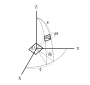
\includegraphics[width=0.7\textwidth]{images/Theory/DirectionalIntensity.pdf}
    \caption[Concept of Directional Intensity and Solid Ange]{This figure shows the concept of the directional intensity and the solid angle in e spherical coordinate system. The drawing is adapted from P.K.F. Grieder's work \cite{CosmicRayGrieder}.}
    \label{fig:DirectionalIntensityConcept}
\end{figure}
The directional intensity is often considered as a function of one of the angles, while the differential of the respective other angle gets integrated. In the case of $I_i(\phi^\prime)$, this usually results in a constant distribution. For $I_i(\theta^\prime)$, however, there is a clear angle dependence. Said zenith angle dependence can be expressed as 
\begin{equation}\label{eq:ThetaDependentIntensity}
    I_i(\theta^\prime) = I_i(\theta^\prime=\SI{0}{\degree}) \cos^{n_{i}}{(\theta^\prime)}.
\end{equation}
The parameter $n_{i}$ differs for various particles, their energies, and the elevation at which $I_i(\theta^\prime)$ is measured.

The third observable used in this work is the \textbf{differential energy spectrum}, $j(E)$. It is defined as the number of particles as a function of energy $dN_i(E)$, per unit Area, $dA$, per unit time, $dt$, per solid angle, $d\Omega^{\prime}$, and per energy interval, $dE$, \cite{CosmicRayGrieder}
\begin{equation} \label{eq:DifferentialEnergySpectrum}
    j_i(E) = \frac{dN_i(E)}{dA \, dt \, d\Omega^{\prime} \, dE}, \quad \left[ \si{\per\centi\metre\squared\per\second\per\steradian\per\giga\electronvolt} \right].
\end{equation}
The differential energy spectrum appears quite similar to the directional intensity, in fact the only noticeable difference seems to be the energy differential $dE$ in the denominator. On closer inspection though, it becomes that $dN_i(\phi^{\prime},\theta^{\prime})$ is the number of particles as a function of angles, while $dN_i(E)$ is the number of particles as a function of energy. Cosmic-ray particle energy spectra can in part be represented by a power law function in energy with a constant exponent $\gamma$ and a form factor $A$ \cite{CosmicRayGrieder}, \ie
\begin{equation} \label{eq:CosmicRayEnergyDependency}
    j(E) = AE^{-\gamma}.
\end{equation}
Therefore, most measured data is fitted to above function, often in different sections of energy. The cosmic primary particle spectrum, for example, is divided into several sections, from \SIrange{100}{3e6}{\giga\electronvolt} the exponent has a value of $\gamma \approx 2.7$. At this point, \ie at \SI{3e6}{\giga\electronvolt}, the so-called \textbf{knee} can be observed, where the dominant particle sources transitions from galactic to extra galactic. Between \SIlist{3e6;e10}{\giga\electronvolt} we find the spectrum slightly steepening from $\gamma \approx 3.0$ to $\gamma \approx 3.15$ at \SI{e9}{\giga\electronvolt}. Finally, beyond the so-called \textbf{ankle} at \SI{e10}{\giga\electronvolt} we again find $\gamma \approx 2.7$.
% TODO Make graph about the primary spectrum

In our use case, it is also interesting to consider the number of particles above a certain energy $E$. This is particularly important while studying backgrounds, since they usually appear above a certain energy threshold, so the number of background events becomes an integrated energy spectrum. For this purpose let us introduce the fourth observable, the \textbf{integral energy spectrum}, $J_i(E)$. It is defined as the integral in energy $dE^{\prime}$ from an $E$ to $\infty$ of $j_i(E^{\prime})$ as follows, \cite{CosmicRayGrieder}
\begin{equation} \label{eq:IntegralEnergySpectrum}
    J_i(E) = \int_{E}^{\infty} dE^{\prime} \ j_i(E^{\prime}) = \frac{dN_i(E^{\prime})}{dA \, dt \, d\Omega^{\prime}} \Biggr|_{E}^{\infty} \quad , \quad \left[ \si{\per\centi\metre\squared\per\second\per\steradian} \right].
\end{equation}
As can be seen, $J_i(E)$ features the same units as $I_i(\phi^{\prime},\theta^{\prime})$, but the both are indeed completely different variables introduced to show completely different purposes of cosmic-rays.

Energy spectra are often measured at different elevations, which has an impact on the form factor $A$ in equation \ref{eq:CosmicRayEnergyDependency} but does not affect the term $E^{-\gamma}$. Furthermore, astroparticle physicists do not use elevation, but \textbf{vertical depth} $X$, also known as \textbf{vertical column density} or \textbf{overburden}. It constitutes the amount of matter traversed by an incident particle along its inclined trajectory subtending a zenith angle $\theta^\prime \approx \SI{0}{\degree}$. $X$ is actually a line integral of the volume density $\rho$ and thus possesses the units of $[\si{\gram\per\centi\metre\squared}]$. Since the atmospheric density decreases exponentially with increasing elevation, our vertical depth is also an exponential function of elevation. At sea-level $X \approx \SI{1000}{\gram\per\centi\metre\squared}$, at an altitude of roughly $\SI{16}{\kilo\metre}$ \gls{asl} one finds $X \approx \SI{100}{\gram\per\centi\metre\squared}$, and $X \approx \SI{10}{\gram\per\centi\metre\squared}$ at around $\SI{32}{\kilo\metre}$ \gls{asl}. So, with every $\SI{16}{\kilo\metre}$ in elevation, $X$ is reduced by a factor of ten \cite{CosmicRayGrieder}. It is obvious, that the vertical depth must exhibit a zenith angle dependence, since a longer distance through the atmosphere has to be traversed if $\theta^{\prime} \neq \SI{0}{\degree}$. This angle dependency is introduced through the \textbf{slant depth} $X_\text{s}$ and simple trigonometry:
\begin{equation}
    X_\text{s} = \frac{X}{\cos{(\theta^\prime)}}.
\end{equation}
Above equation is only valid for $\theta^\prime \leq \SI{60}{\degree}$, where the earth's - and thus the atmosphere's curvature is negligible \cite{CosmicRayGrieder}.

For the altitude dependence let us consider intensities once again, as they show an obvious angle dependency. The intensity of a hadron $i$ measured at a vertical depth $X_1$, $I_i(\theta^\prime=\SI{0}{\degree}, X_1)$, can be transformed into $I_i(\theta^\prime=\SI{0}{\degree}, X_2)$ at a grater depth $X_2$ by \cite{CosmicRayGrieder}
\begin{equation} \label{eq:AltitudeDependency}
    I_i(\theta^\prime=\SI{0}{\degree}, X_2) = I_i(\theta^\prime=\SI{0}{\degree}, X_1) e^{-\frac{X_2-X_1}{\Lambda}}.
\end{equation}
Here, $\Lambda$ stands for the particle dependent attenuation length in units of $\si{\gram\per\centi\metre\squared}$. When using $X_\text{s}$, an angle dependence can be introduced. In addition, one can also apply above operations to energy spectra $j_i(E)$ and $J_i(E)$.

While above observables are useful to compare cosmic-ray measurements of different experiments, they are not suitable to illustrate cosmic-ray background in a single experiment like MicroBooNE. Neutrino experiments usually count events in a predetermined \textbf{fiducial volume} over a time period (see section \ref{sec:MeasuringCrossSection}). Therefore, we are, for example, not interested in the area differential. Since background cuts are applied on single variables at the time we also only consider single differentials, with the exception of $d\Omega$ which is by definition a double differential. In our case it is thus more useful to consider event rates in the \textbf{fiducial volume} $r_i$ as our base observable rather than the more complex intensities discussed above. Here the letter $i$ again denotes the particle flavour and moreover, I introduce my own notation. A rate is generally defined as
\begin{equation} \label{eq:Rate}
    r_i = \frac{dN_i}{dt}, \quad \left[ \si{\per\second} \right],
\end{equation}
where again $dN_i$ stands for the number of particles and $dt$ for the time interval. In order to accommodate different distributions, we can also introduce differential rates, analogous to the differential intensities and spectra introduced above. One of these is the \textbf{differential volume rate},
\begin{equation} \label{eq:DifferentialVolumeRate}
    \frac{dr_i(V)}{dV} = \frac{dN_i(V)}{dt \, dx \, dy \, dz}, \quad \left[ \si{\per\centi\metre\cubed\per\second} \right],
\end{equation}
with $dx$, $dy$, and $dz$ denoting the differentials of the three spacial coordinates. It is used to visualise the rate within a detector volume, wherefore one of the coordinate differentials is usually integrated, as said visualisations are often simplified to \gls{2d} views. An other often used observable of cosmic background events in a detector is their angular rate distribution, analogous to the directional intensity of equation \ref{eq:DirectionalIntensity}, and defined by
\begin{equation} \label{eq:DifferentialDirectionalRate}
    \frac{dr_i(\phi,\theta)}{d\Omega} = \frac{dN_i(\phi,\theta)}{dt \, d\phi \, d \theta \, \sin{\left(\theta\right)}}, \quad \left[ \si{\per\second\per\steradian} \right].
\end{equation}
Let us call above observable \textbf{differential directional rate}. Note that the angles $\phi$ and $\theta$ as well as the solid angle $\Omega$ now denote those of the MicroBooNE coordinate system which is rotated horizontally with respect to the astroparticle physics reference system. Analogous to the differential energy spectrum in equation \ref{eq:DifferentialEnergySpectrum} we define the \textbf{differential energy rate} as
\begin{equation} \label{eq:DifferentialEnergyRate}
    \frac{dr_i(E)}{dE} = \frac{dN_i(E)}{dt\,dE}, \quad \left[ \si{\per\second\per\giga\electronvolt} \right].
\end{equation}
Finally, let us introduce the rate equivalent of the integral energy spectrum of equation \ref{eq:IntegralEnergySpectrum}, the \textbf{integral energy rate}, $R_i$, as
\begin{equation} \label{eq:IntegralEnergyRate}
    R_i(E) = \int_{E}^{\infty} dE^{\prime} \ \frac{dr_i(E^{\prime})}{dE^{\prime}} = \frac{dN_i(E^{\prime})}{dt}\Biggr|_{E}^{\infty}\quad , \quad \left[ \si{\per\second} \right].
\end{equation}
With these parameters established, we are now ready to investigate the \gls{mc} simulation of the cosmic-ray gamma background in section \ref{sec:CosmicRayGammaBackground}.

% TODO explain that this coordinate system takes the observer as a point of reference (observing from wich angles, the radiation comes in). MicroBooNE uses the opposit: observing which angles a particle travels from the coordinate system's origin.
